\documentclass[12pt]{ucthesis}

\usepackage{etex}
\usepackage[morefloats=125]{morefloats}
\usepackage[hyphens]{url}
\usepackage{subfig}
\usepackage{graphicx}
\usepackage{tabularx}
\usepackage{amssymb}
\usepackage{amsmath}
\usepackage[letterpaper]{geometry}
\usepackage[overload]{textcase}
\usepackage{color}
\usepackage[nonumberlist,toc]{glossaries}
\usepackage{wrapfig}
\usepackage{longtable}
\usepackage{morefloats}
\usepackage{float}
\usepackage{listings}
\usepackage{makecell}
\usepackage{appendix}
\usepackage[]{algorithm2e}
\usepackage{titlesec}
\usepackage{microtype}
\usepackage{lmodern}
\usepackage[breaklinks=true,hidelinks,pdfusetitle]{hyperref}
\usepackage{cleveref}
\usepackage{ifthen}
\usepackage{booktabs}
\usepackage{inconsolata}

\setcounter{secnumdepth}{3}
\setcounter{tocdepth}{3}

\makeindex
\makeglossaries

% Shrink the size of headers
\titleformat{\chapter}[display]
        {\normalfont\normalsize\centering}
        {\ifthenelse{\equal{\thechapter}{A}}{APPENDICES\\[4.3ex]}{}\chaptertitlename\ \thechapter}
        {0pt}{\normalsize\uppercase}
\titlespacing*{\chapter}{0pt}{-20pt}{4.3ex plus .2ex}


\titleformat*{\section}{\normalsize\bfseries}
\titleformat*{\subsection}{\small\bfseries}
\titleformat*{\subsubsection}{\small\bfseries}
\titleformat*{\paragraph}{\small\bfseries}
\titleformat*{\subparagraph}{\small\bfseries}

\bibliographystyle{abbrv}

% Make \tindent indent pages if you have no paragraph indent
\newlength\tindent
\setlength{\tindent}{\parindent}
\setlength{\parindent}{0.in} \setlength{\parskip}{1.em}
\renewcommand{\indent}{\hspace*{\tindent}}
% Otherwise, comment out the above and uncomment this for default indentation on each paragraph
%\setlength{\parindent}{0.25in} \setlength{\parskip}{6pt}

\geometry{verbose,nohead,tmargin=1in,bmargin=1in,lmargin=1.5in,rmargin=1in}

% Different font in captions (single-spaced, bold) ------------
\newcommand{\captionfonts}{\small\bf\ssp}

\newcommand{\mycaption}[2]{\caption[#1 --- #2]{#1 --- #2}}

\makeatletter  % Allow the use of @ in command names
\long\def\@makecaption#1#2{%
  \vskip\abovecaptionskip
  \sbox\@tempboxa{{\captionfonts #1: #2}}%
  \ifdim \wd\@tempboxa >\hsize
    {\captionfonts #1: #2\par}
  \else
    \hbox to\hsize{\hfil\box\@tempboxa\hfil}%
  \fi
  \vskip\belowcaptionskip}
\makeatother   % Cancel the effect of \makeatletter
% ---------------------------------------

% Define Appendix refs
\crefname{app}{appendix}{appendices}
\Crefname{app}{Appendix}{Appendices}

% Add Figures folder to the graphics path
\graphicspath{{Figures/}{figures/}}

% Options for hyperref
\hypersetup{
    bookmarksnumbered=true,
    bookmarksopen=false,
    bookmarksopenlevel=0,
    colorlinks=false,
    pdfstartview=Fit,
    pdfborder={0 0 0},
}

\newcounter{qcounter}
\providecommand{\keywords}[1]{\textbf{\textit{Keywords:}} #1}

\definecolor{mygreen}{rgb}{0,0.6,0}
\definecolor{mygray}{rgb}{0.5,0.5,0.5}
\definecolor{mymauve}{rgb}{0.58,0,0.82}

\lstset{ %
  language=Python,
  showstringspaces=false,
  numbers=left,
  stepnumber=1,
  backgroundcolor=\color{white},   % choose the background color
  basicstyle=\ttfamily\linespread{0.85},
  breaklines=true,                 % automatic line breaking only at whitespace
  captionpos=b,                    % sets the caption-position to bottom
  commentstyle=\color{mygreen},    % comment style
  escapeinside={\%*}{*)},          % if you want to add LaTeX within your code
  keywordstyle=\color{blue},       % keyword style
  stringstyle=\color{mymauve},     % string literal style
  frame = single,
}

\begin{document}

% Declarations for Front Matter
\title{Logging, Visualization, and Analysis of Network/Power Data of IoT Devices}
\author{Neal Nguyen}
\degreemonth{December} \degreeyear{2018} \degree{Master of Science}
\defensemonth{November} \defenseyear{2018}
\numberofmembers{2}
   \chair{Andrew Danowitz, Ph.D. \linebreak Assistant Professor of Electrical Engineering}
   \othermemberA{Bruce Debruhl, Ph.D. \linebreak Assistant Professor of Computer Science}
   \othermemberB{Lynne Slivovsky, Ph.D. \linebreak Professor of Electrical Engineering}
\field{Electrical Engineering} \campus{San Luis Obispo}
\copyrightyears{seven}


\maketitle

\begin{frontmatter}

% Custom made for Cal Poly (by Mark Barry, modified by Andrew Tsui).
\copyrightpage

% Custom made for Cal Poly (by Andrew Tsui).
\committeemembershippage

\begin{abstract}
It is estimated that there are 23.14 billion IoT(Internet of Things) devices currently in use worldwide. This number is projected to grow to over 75 billion by 2025. Despite their ubiquity little is known about the security and privacy implications of IoT devices. Several large scale attacks against IoT devices have already been recorded.

To help address this knowledge gap, we have collected a year’s worth of network traffic and power data from 16 common IoT devices. From this data, we show that we can identify different smart speakers, like the Echo Dot, from analyzing one minute of power data on a shared power line.
\end{abstract}

\begin{acknowledgements}
\noindent
Thanks to:
\begin{itemize}
    \item My parents for supporting me throughout life. I wouldn't have made it here without your time and effort.
    \item Ryan Frawley for setting up the scripts for device logging and analysis alongside me. You really set a strong foundation for us to build upon!
    \item Cal Poly and Cisco for funding this project. We would not have had the resources needed to accomplish our task.
\end{itemize}

\end{acknowledgements}

\tableofcontents

\listoftables

\listoffigures

\lstlistoflistings

\addcontentsline{toc}{chapter}{LIST OF CODE LISTINGS}

% Add CHAPTER into table of contents.
\addtocontents{toc}{%
   \noindent CHAPTER
}

\end{frontmatter}

\pagestyle{plain}

\renewcommand{\baselinestretch}{1.66}

\chapter{Introduction}
\label{Introduction}
There are 23.14 billion IoT devices in use worldwide that nubmer is expected to grow to 75.44 billion by 2025 \cite{statista_2016}. With so many manufacturers creating IoT devices, each with differing update policies, some devices inadvertently have better support. For example, some devices may drop out of a manufacturer's update cycle and become unsupported, introducing privacy and security concerns.

To address these concerns, this thesis contributes an IoT testbed that logs network and power data from 16 IoT devices over one year, accumulating 184.94 GB of data and 172,445,929 rows into a database. To help researchers sort and view this data, this thesis adds a Python program that graphs network traffic and power data over time from the database. The graphs created by this tool were used to analyze IoT devices network and power usage in the testbed while idle, during startup, and while in use. From these graphs, it is possible to identify the smart speaker in use when viewing just one minute of the shared power usage.

This paper focuses on addressing security and privacy flaws, that if fixed, do not affect the core features of an IoT device. For example, a smart speaker must store audio snippets to parse for the wake word. If the smart speaker occasionally hears a false positive wake word and sends the audio to its server, that is reasonable. However, Google Homes had an issue with their wake button, which caused the Home to listen 24/7 \cite{burke_2017}. This is not expected behavior and highlights privacy concerns. In another case, one of the largest IoT cybersecurity attacks, Mirai, was able to use weak login credentials to take control of 2.5 million IoT devices to perform a denial of service attack \cite{whittaker_2017}. This is on many events that introduces security concerns. This paper uses these flaws as a focus when analyzing network and power usage.

\section{Previous Work}
This section presents and analyzes related works on the topic of analyzing and characterizing IoT devices. It presents the previous works individually. Because these papers are similar to each other, commentary on how their work is different from ours and how it is useful to us as a group in section \ref{Scope}.

\subsection{An Analysis of Home IoT Network Traffic and Behaviour}
\label{homeIoTPaper}
The scope and work of \textit{An Analysis of Home IoT Network Traffic and Behaviour}~\cite{home_iot} are most like the work and goals of this paper. In \textit{An Analysis of Home IoT Network Traffic and Behaviour}~\cite{home_iot}, the authors analyze IoT traffic in the home. The authors created an IoT testbed by setting up multiple IoT devices, connecting them to a router, sniffing their network packets while idle, and storing these packets on a Linux box's disk. The IoT testbed consists of a smart air quality monitor, Amazon Echo, a few Apple devices, a smart hub, and a smart vacuum cleaner.

After 22 days of network logging, the authors analyzed each IoT device individually and as a whole. For example, they noticed that they can identify most devices from the first three MAC address bits. The Hue bridge broadcasts credentials over HTTP, which is unencrypted. The authors state that these seemingly small security flaws create a privacy risk. A user’s presence in a room or house can be determined from these unencrypted HTTP packets. The authors also show the percentage of network packets by protocol and various other device network patterns. This general analysis fingerprints each device.

\subsection{ProfilIoT}
\label{ProfilIoTPaper}
The paper, \textit{ProfilIoT: A Machine Learning Approach for IoT Device Identification Based on Network Traffic Analysis} ~\cite{Meidan:2017:PML:3019612.3019878} uses machine learning algorithms to classify IoT devices. The researchers of this paper collect traffic from 13 different IoT and non-IoT devices. The IOT devices include a baby monitor, motion sensor, printer, refrigerator, security camera, socket, thermostat, smartwatch, and television. The non-IoT devices include two PCs and two smartphones for comparison. These devices connect to a Wi-Fi access point that recorded their network traffic with Wire Shark\cite{wireshark}.

The researchers use machine learning on single-sessions to classify a device as an IoT device or non-IoT device. Then, they can classify the IoT devices by brand and model(e.g. Samsung Refrigerator, LG TV, WeMo Motion Sensor) with multi-sessions. A single-session is a 4-tuple formatted as source IP, destination IP, source port Number, destination port Number. When intercepting network traffic, they extracted the information they needed from each TCP packet to form the four-tuple data type. A multi-session is a list of single-sessions. Another machine learning model determines the minimum number of single-sessions needed to classify each device, determining the size of a multi-session. With single-sessions, they could determine if the device is an IoT device or not with 100 percent accuracy. Then out of their nine IoT devices, they can classify brand and model of the IoT device with 99.281 percent accuracy when run 7376 times.

\subsection{Logging and Analysis of Internet of Things (IoT) Device Network Traffic and Power Consumption}
\label{frawleyPaper}
\textit{Logging and Analysis of Internet of Things (IoT) Device Network Traffic and Power Consumption}\cite{frawley_2018}, written by Ryan Frawley, was formed in conjunction with this paper. Frawley's paper and this paper were both directed by advisor Andrew Danowitz at Cal Poly.

Frawley's paper documents the steps necessary to construct a reliable IoT testbed capable of capturing network traffic and power data for connected devices, and analyzing these devices further. He performed GeoIP\cite{maxmind} lookups on each device, showing the percentage of packets originating from each country and company. He also analyzed the packets of any unencrypted data in the devices.

\section{Scope}
\label{Scope}
The first paper from subsection \ref{homeIoTPaper} most closely matches this paper. The authors have the same overall idea to collect network data and then use it to analyze metadata surrounding the networks. Our work expands on this concept by contributing a portable database consisting of 10 months of data rather than 22 days of data. This paper adds more devices in our study and focuses more on device power/network usage over time rather than specific network packet information.

Then, like the second paper from subsection \ref{ProfilIoTPaper}, this paper also focuses on classification of devices from data. However, instead of using machine learning techniques on network data, this paper focuses on manual analysis, looking for spikes in power usage, the height of the spike, the length of the power spike, and other graphical heuristics.

In comparison to the first paper in \ref{homeIoTPaper} and second paper in \ref{ProfilIoTPaper}, this paper adds power usage over time to the data set. The two papers mentioned only focus on network traffic. This paper also puts a significant emphasis on creating an extensive database rather than a smaller set of data to create graphs on network and power usage over time.

This paper is a continuation of the third paper in subsection \ref{frawleyPaper}. Due to overlap between these two works, certain aspects of the IoT testbed setup and usage is only covered in cursory detail here. The reader is advised to access Frawley's work for full information. We both assembled the IOT test bed and interacted with the devices on a daily basis to simulate regular usage. We both also performed a preliminary analysis of the device network and power usage together.

The unique contribution of this work is its analysis of IoT device power usage and the introduction of a custom data visualization tool that attaches to the database. This paper focuses on a select few devices, analyzing their startup, idle, and in use network and power usage over time. I compare the smart speakers' network and power usage and show that it is possible to identify a smart speaker through analysis of the powerline over time.

\section{Thesis Organization}
Chapter \ref{Method} discusses my steps in setting up the IOT test bed, the analysis tool, and the logging system for interaction with devices. Chapter \ref{Method} also highlights the steps to set up a developer environment to run the analysis tool and how to use it. Chapter \ref{Results} presents power and network traffic for smart speakers and streaming devices while idle, in use, and during startup in the form of line graphs. Chapter \ref{Results} also shows the graphs used to fingerprint the smart speakers while handling different commands and under noise. Chapter \ref{Discussion} discusses the data presented in Chapter \ref{Results}, why a device might have higher throughput traffic and the feasibility of classifying devices within a household from a shared power line. Finally, Chapter \ref{Conclusion} finishes with concluding thoughts and future work.

\chapter{Method}
\label{Method}
The flow diagram in figure \ref{fig:network} outlines the IoT test bed constructed for this project. IoT devices pull power from the outlets through the smart switches, which log the power usage, and the WAP will query the smart switches for that data and pushes it to an AWS (Amazon Web Services)\cite{rds} MySQL\cite{mysql} database as an entry in the `power' table.

The wireless net provided through the WAP intercepts network packets of devices connected to it (IoT devices in testbed), parses them into power and network entries, and pushes them to the database. Finally, for analysis, a python script called realTimeGrapher.py pulls from the database and graphs this data in real time or from set intervals in the past.

Section \ref{Physical Layout and Setup} discuss what devices we used, the setup of each device, and the physical layout of the IoT test bed. Section \ref{software} will go over the software part of the IoT test bed. It covers the usage flow of this test bed and what was done to obtain results for analysis.

\begin{figure}[H]
    \centering
    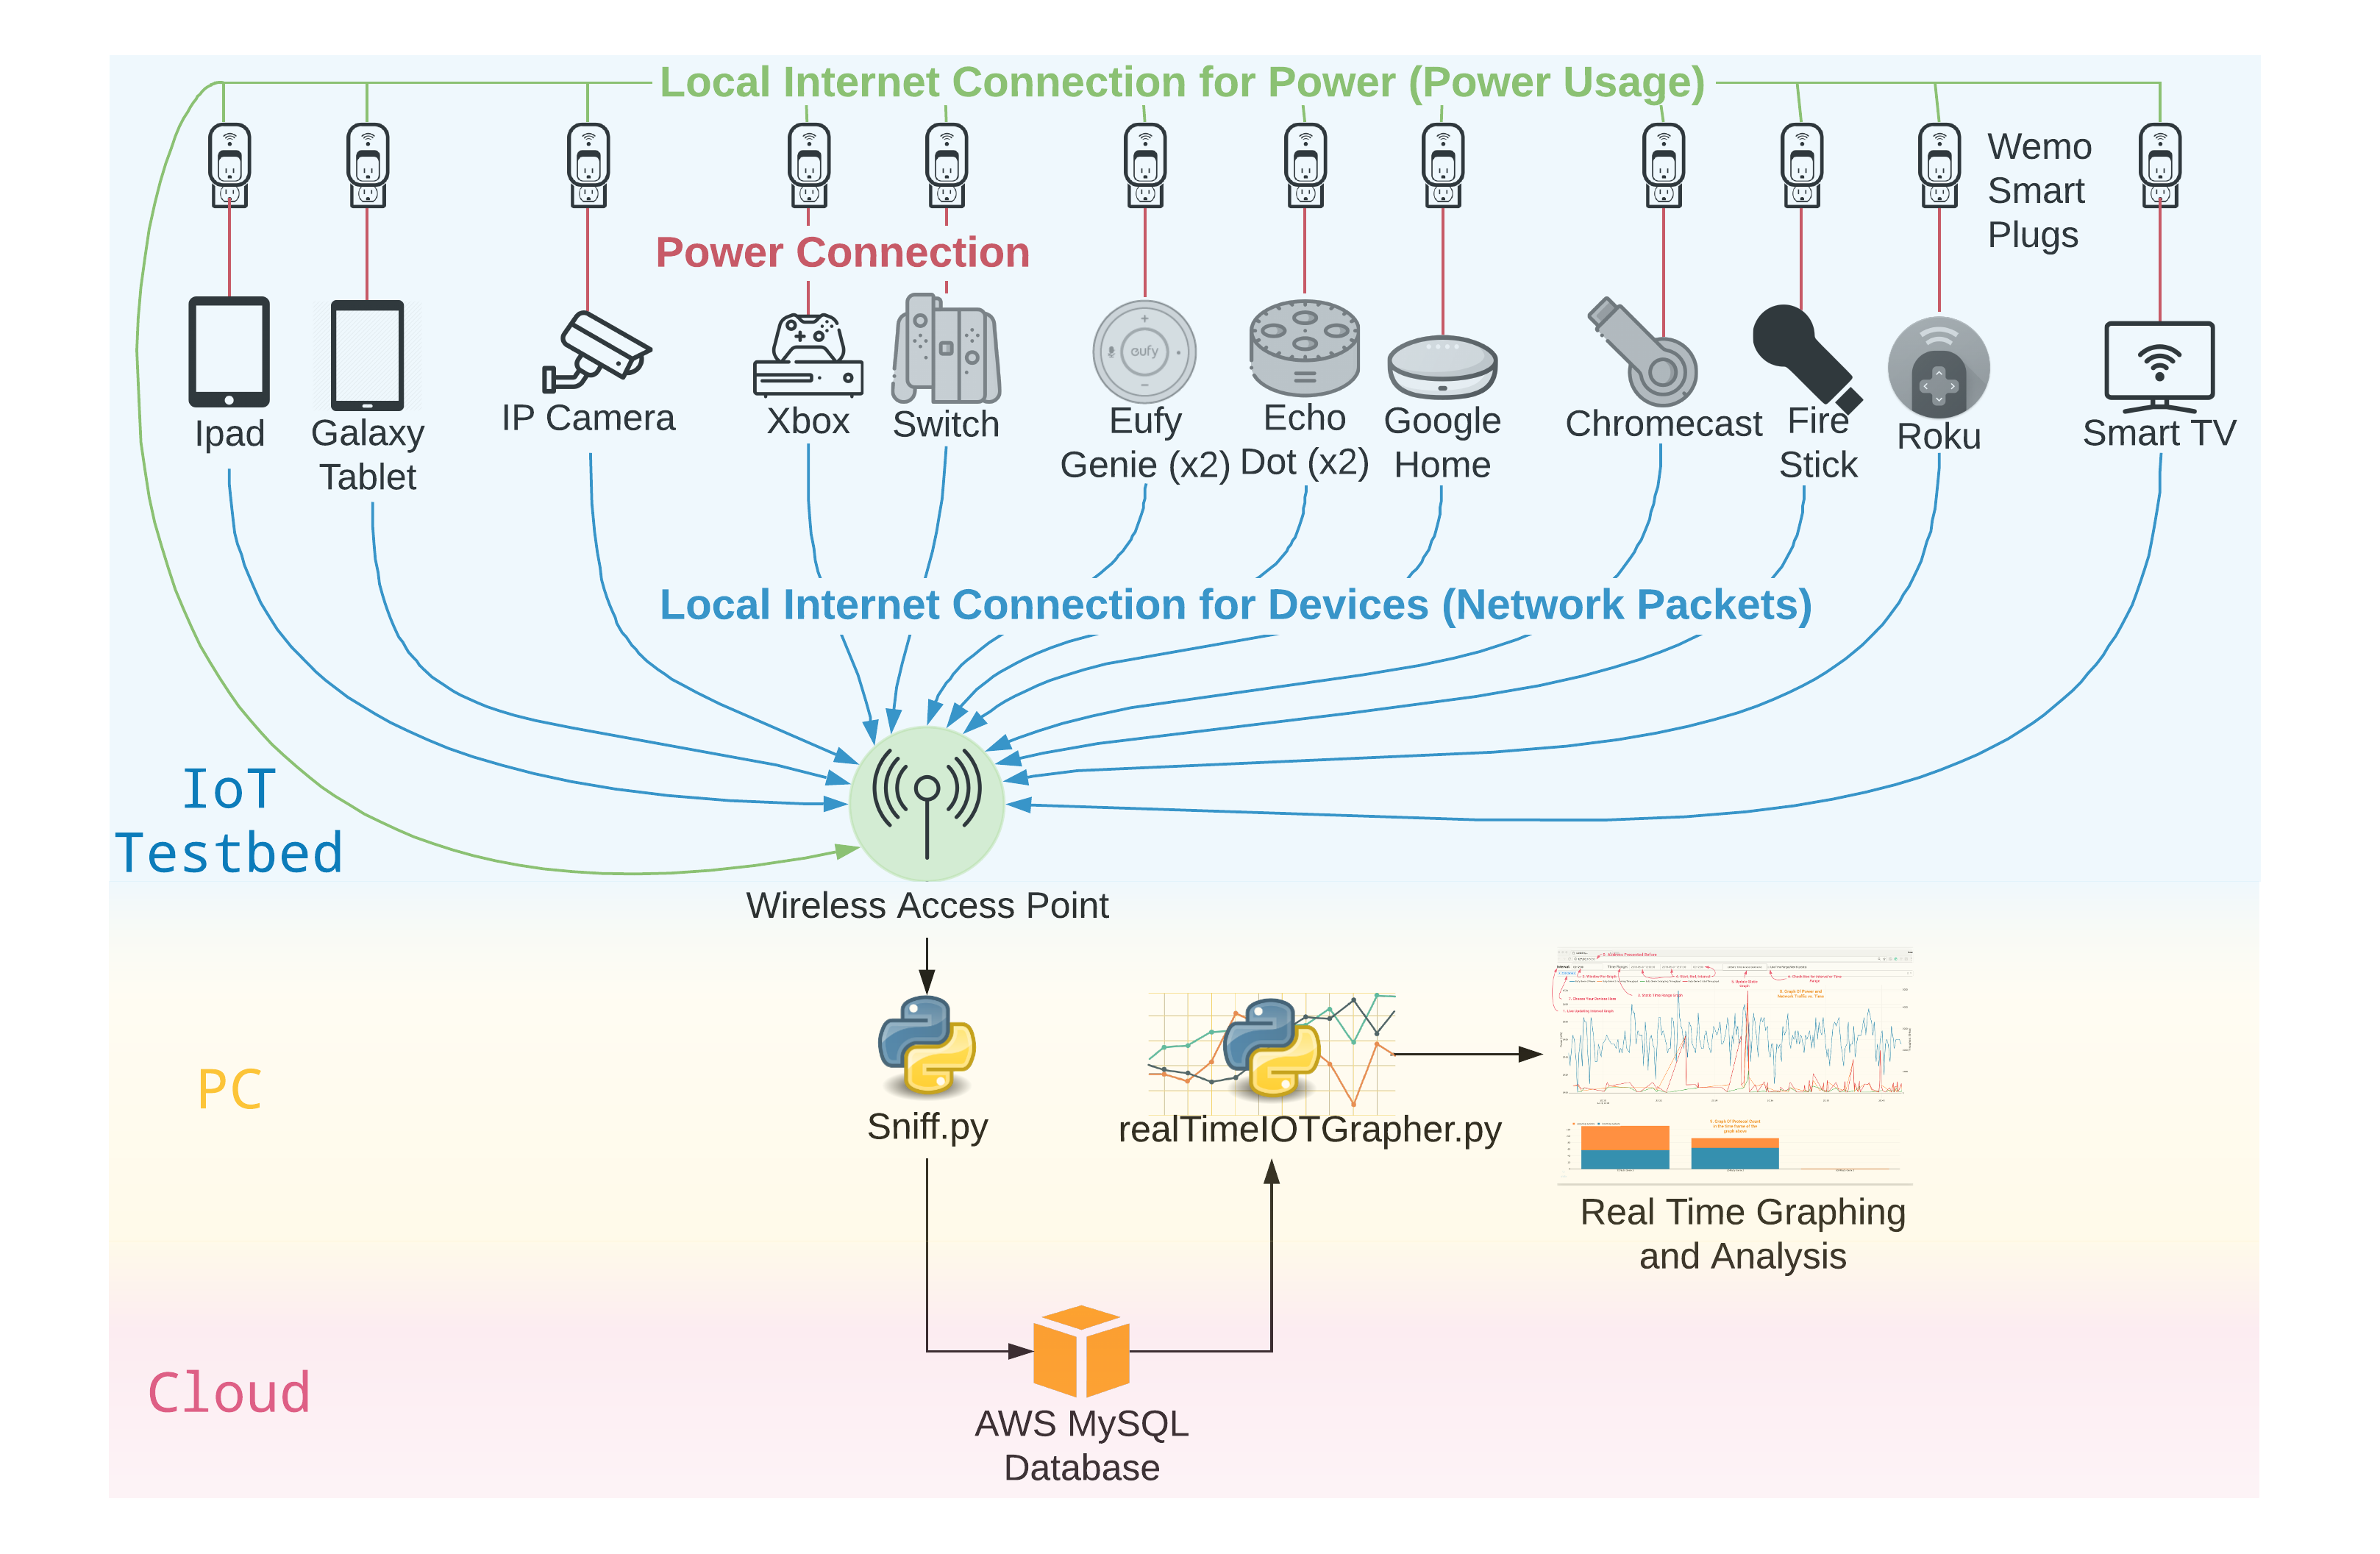
\includegraphics[width=1.0\textwidth]{networkDiagram}
    \caption{Network Diagram}
    \label{fig:network}
\end{figure}

\begin{figure}[H]
    \centering
    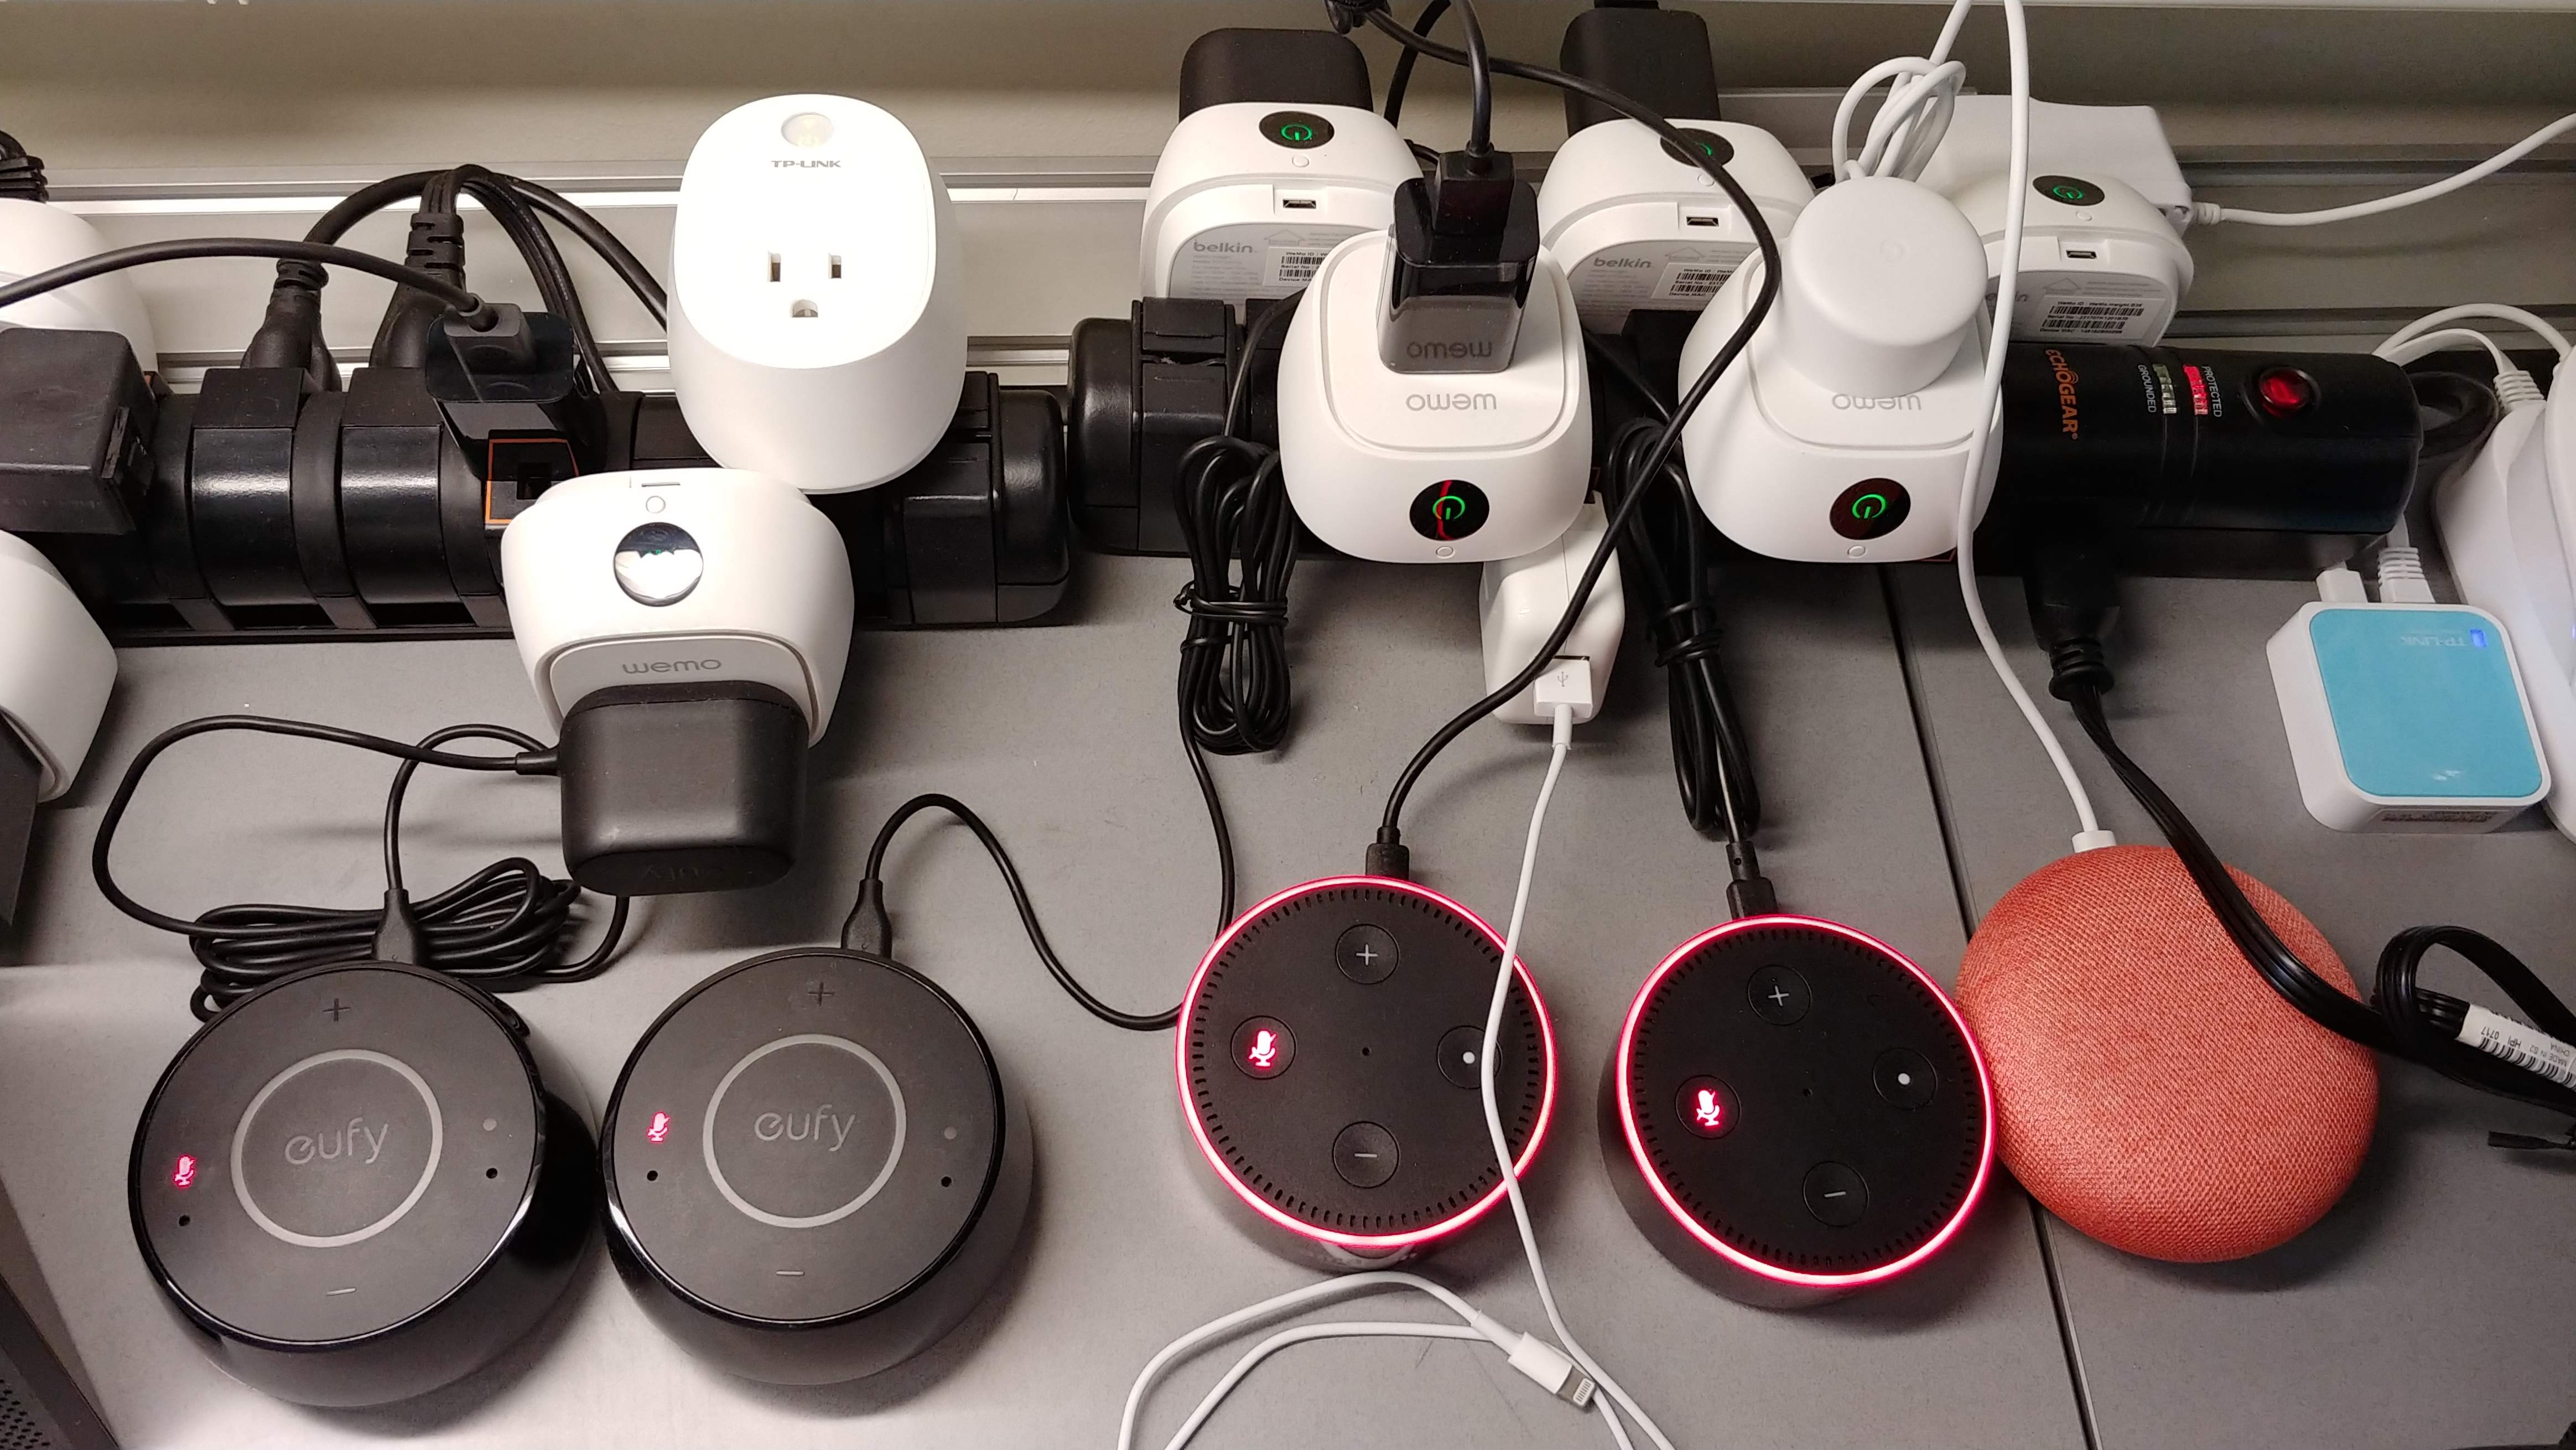
\includegraphics[width=1\textwidth]{wemos}
    \caption{Smart Speakers Connected to WeMo Insight Switches}
    \label{fig:wemo}
\end{figure}

\begin{figure}[H]
    \centering
    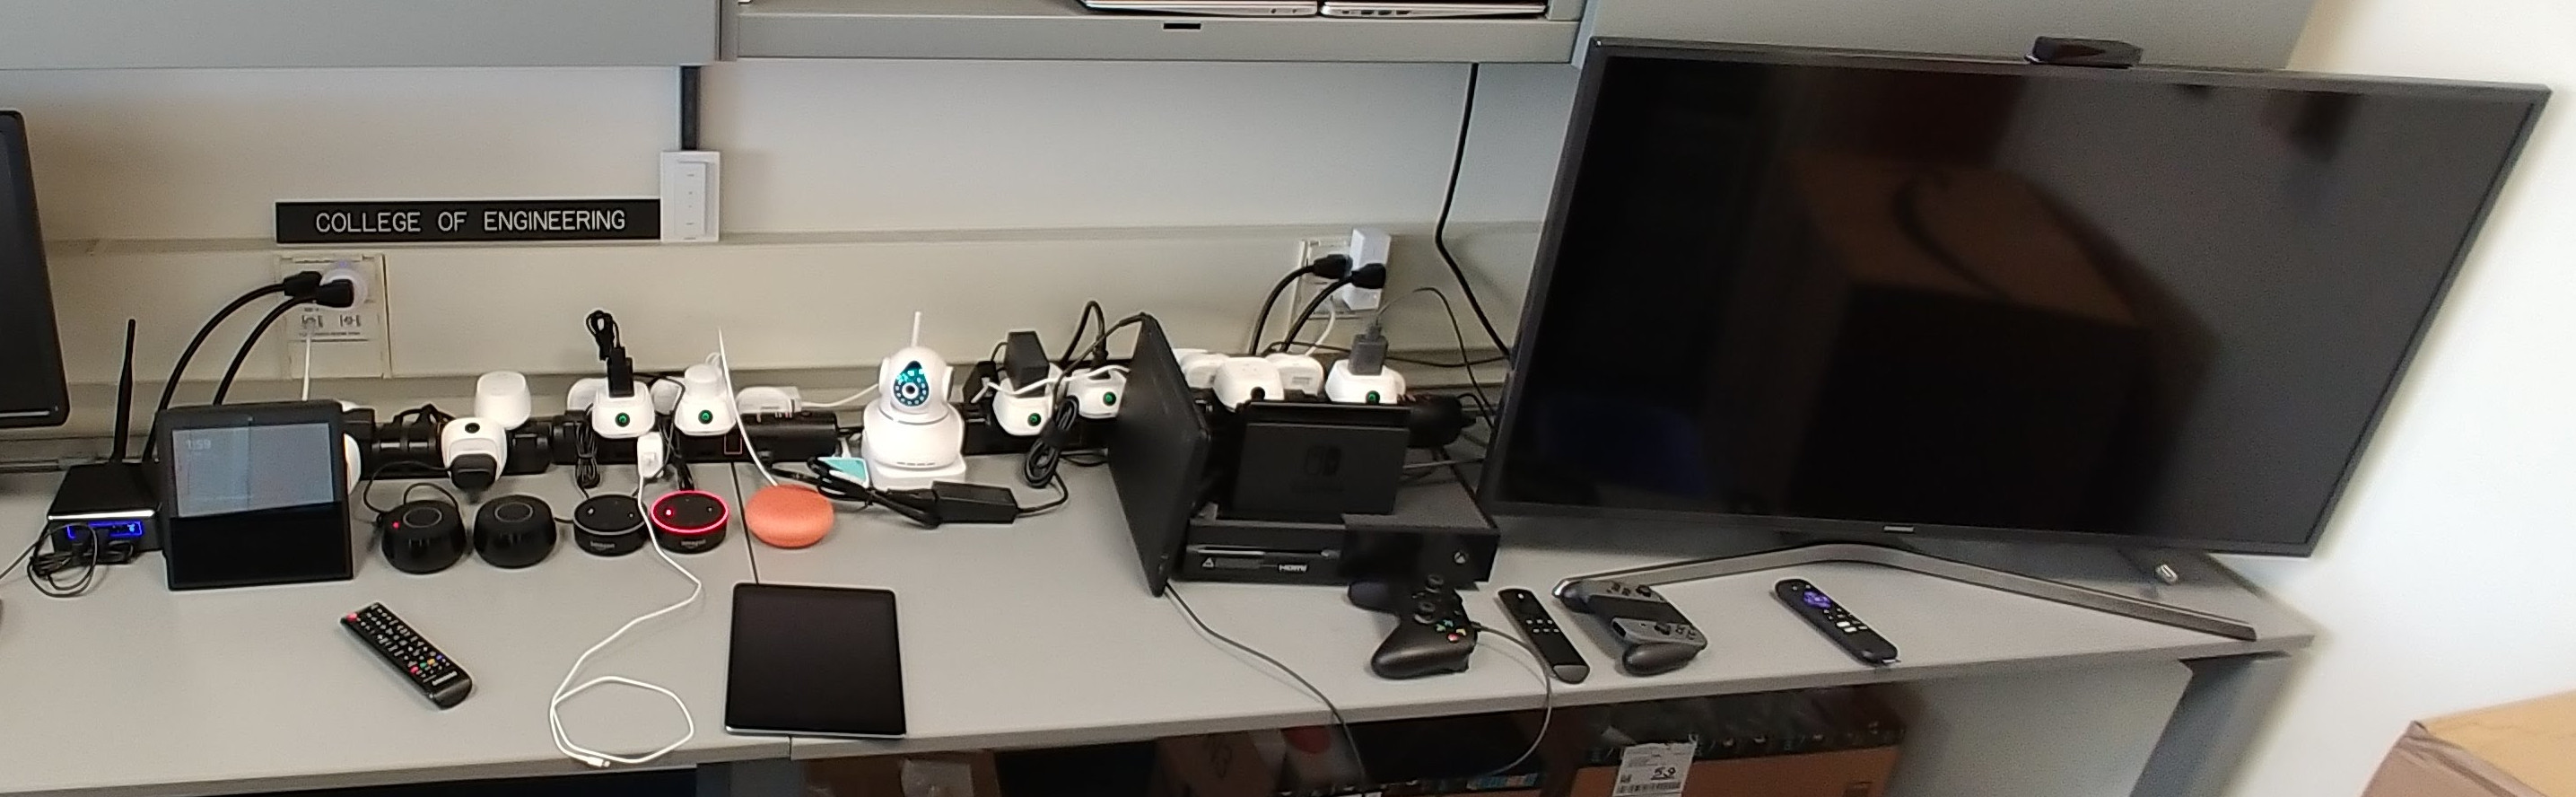
\includegraphics[width=1\textwidth]{devices}
    \caption{IoT Devices Under Examination}
    \label{fig:devices}
\end{figure}

\section{Physical Layout and Setup}
\label{Physical Layout and Setup}

This section covers the physical setup and layout of the hardware used when setting up the IoT test bed, the IoT devices we tested, and how each device is set up. Figures \ref{fig:wemo} and \ref{fig:devices} show the IoT testbed set up. Setup was performed with Ryan Frawley and explained in his paper \ref{frawleyPaper}, this paper provides an updated description.

\subsection{Wireless Access Point}
\label{Wireless Access Point}
The wireless access point is an Intel NUC \cite{nuc}. We loaded Ubuntu\cite{ubuntu} on it because it is the most common Linux OS \cite{linux} and most flexible for developing scripts and programs to log network packets, query power information, and push those values to a database.

One challenging thing about the NUC is that its internal wireless chip is very slow. The throughput when using the wireless chip was measured to be 12 Mb/s down on Speedtest.net by Ookla \cite{speedtest} when connected to with a Chromebook \cite{chromebook} (25 Mb/s is the minimum possible for broadband). This rate limitation caused many of the Belkin WeMo smart switches \cite{wemo} to drop their connection intermittently, causing gaps in recorded power data. To solve this, we added a USB wireless antenna to the NUC. This antenna improved our internet speed to 30 Mb/s down when tested on Speedtest.net by Ookla with the same Chromebook, solving the issue where devices would lose network connectivity.

\subsection{Devices}
\label{Devices}
This section goes over the smart speakers, streaming devices, video game consoles, tablets, security cameras, or other devices as listed in figure \ref{tab:devices}. These devices were included based on their popularity, as the goal of the paper is to build a data set from common household IoT items.

\begin{table}[H]
    \centering
    \caption{IoT Devices Being Monitored}
    \begin{tabular}{@{}llll@{}}
    \toprule
    Category & Manufacturer & Device        & Quantity \\ \midrule
    Game Console & Nintendo     & Switch        & 1        \\
    Game Console & Microsoft    & Xbox One      & 1        \\
    Laptop & HP           & Chromebook    & 1        \\
    Media Player & Samsung      & Smart TV      & 1        \\
    Media Player & Google       & Chromecast    & 1        \\
    Media Player & Amazon       & Fire TV Stick    & 1        \\
    Media Player & Roku         & Express       & 1        \\
    Security Camera & Eray    & Hi3518 Wi-Fi Camera     & 1        \\
    Smart Speaker & Amazon       & Echo Dot      & 2        \\
    Smart Speaker & Eufy/Anker   & Genie         & 2        \\
    Smart Speaker & Amazon       & Echo Show     & 1        \\
    Smart Speaker & Google       & Home Mini     & 1        \\
    Tablet & Amazon       & Fire 7 Tablet & 2        \\
    Tablet & Samsung      & Galaxy Tablet & 1        \\
    Tablet & Apple        & iPad          & 1        \\ \bottomrule
    \end{tabular}
    \label{tab:devices}
\end{table}

\subsubsection{Smart Speakers}
\label{Smart Speakers}

Smart speakers are IoT devices that combine speakers with built-in voice assistants, such as Amazon Alexa, Google Assistant, or Apple's Siri. These devices are mainly controlled by voice commands, preceded by a wake word such as ``hey Google''.

Currently, around 39 million people (16 percent of the US population) use smart speakers\cite{perez_2017}. It is one of the top-selling IoT devices and it can act a central voice control for other IoT devices. In 2022 it is projected that 70 million US households will have at least one smart speaker (55 percent of US households) and around 175 million smart speakers total\cite{perez_2018}. For these reasons, we included this group of devices in our research.

Within the smart speaker category, we included the Amazon Echo Dot, Google Home, and Eufy Genie. The Amazon Echo dot and the Google Home are the two leading smart speaker products. We added the Eufy Genie because it is an Amazon Alexa device that we can compare with the Echo Dot. We also included the Amazon Show, which is a voice assistant with a screen.

\subsubsection{Streaming Devices}

Streaming devices are IoT products that connect to a television or are built into a television (smart TVs) and streams videos or music from online services. In 2017 it was recorded that 70 million US households (58.7 percent of homes) had a television connected to streaming devices \cite{lynch_2017}.

The specific streaming devices we look at include the Roku Express, Amazon Fire TV, and the Google Chromecast. These devices represent three popular streaming platforms (Roku, Google Chromecast, Amazon Fire TV) that have a combined user base of over 110 million users who watch content at least once a month \cite{emarketer_2017}.

To view content from these streaming devices, we use a Samsung smart TV. This TV also as streaming capabilities which we log but do not analyze in this paper.

\subsubsection{Video Game Consoles}

Video game consoles are systems specifically built to play video games. We use two out of the three most popular gaming devices including the Nintendo Switch which sold 17.8 million units \cite{nintendo} and the Xbox One, which sold 30 million units \cite{souppouris_2016} as of January 2018.

\subsubsection{Tablets}

Tablets are devices that have phone operating systems running on them such as the Apple iPad, Samsung Galaxy tablet, and the Amazon Fire tablet. These devices were used for interacting with the other IoT devices, which require a smartphone or tablet for set up or control. Some of the IoT devices are limited to either Android, which runs on the Galaxy, or IOS, which runs on the iPad. Although there is no analysis on these devices in the paper, the network packets are logged. There is no way to track the power usage of these devices because they run on battery.

\subsubsection{Security Camera}

Security cameras are cameras meant to run constantly as surveillance, streaming the video footage so a user can view it from any connected device at any time. Two out of the five largest recorded cybersecurity attacks targeted security cameras \cite{guest_2018}. The specific camera we use is the Eray camera. It is a generic Alibaba device with a weak username:password of admin:1234. A weak username and password make it very susceptible to cyber-attacks. There have also been reports that smart cameras have been found to send unencrypted data \cite{feamster_2016}. We selected this device because it has weak login credentials and is susceptible to Mirai. We wanted to see if it would get hacked by Mirai or some other attack, but we found no indication of such.

\subsubsection{Other Devices}

We also connected several other devices that are harder to categorize, analyze, or both.

We have a smart hub connected to a smart lock, an indoor room temperature sensor, and smart LED light bulbs. These devices are difficult to analyze because they communicate with the smart hub through Zigbee or Bluetooth at which point the smart hub aggregates the data and communicates with the network. To look at the network traffic caused by smart lights individually, we prevented all devices besides the smart LED bulbs from communicating with the smart hub. This isolation minimized other packet noise to the smart hub so that we can monitor the smart hub traffic as a replacement for the smart LED bulbs. However, even then, the smart hub might have extra overhead for other tasks, making isolated analysis difficult.

We also have a Chromebook which we used to control the Chromecast. However, because this is more a laptop than an IoT device, we decided to leave this out of our research

\subsection{Smart Power Plugs}

Smart power plugs are Wi-Fi capable, pass through outlets that another device plugs into. The outlets collect and transmit power usage over the network. They are critical to the power consumption logging in this research.

We used the Belkin WeMo Insight. We chose this smart plug because there are many open source Python libraries for pulling power information from them, and they are relatively affordable.

When setting these smart plugs up, we named each smart plug based on the device connected to it so that when we pull power information with our scripts, we can easily reference data to a smart plug. This informal naming led to issues when the wrong device is connected to the wrong smart plug, as discussed in section \ref{realtimeIoTGrapher.py}

\subsection{Wiring and Configuration}

We also tried to set static IPs for each device, but we decided that the average user would not set up a static IP for their device and left dynamic IPs.

The next step was to setup each device and corresponding smart plug through their corresponding setup application, filling in the device's, user name, email, network configuration, etc. We used the device's name as its user name, e.g. the Echo Dot was given the username ``Echo Dot''.

When plugging in all the devices for the first time for power, we worked to plug each device into the corresponding WeMo smart plug and connected to our WAP during device set up so that we could instantly log power and network traffic information. It was essential to log power as soon as possible to capture a first-boot power profile for each device. Some devices had already been used, so they do not contain startup information(Xbox and the Echo Dot 1).

Set up and configuration took up a significant portion of the research time. We worked to set up each device with a separate email account. To do this, we made around 20 AOL accounts. We wanted email addresses that were not under control of the manufacturer of any of the devices. For example, we did not want to use any Gmail accounts because we did not want the Google Home or Google Chromecast to perform domain-specific optimizations. When setting up AOL accounts, we also faced a limitation of the number of email accounts tied to a single phone number. We had to use different phone numbers to circumvent this.

We set up each device in waves, taking around a week to set everything up. Incremental device setup with no plan resulted in a messy work environment, which made it difficult to match a device to it is corresponding smart plug. After a month of data logging in a disorganized scheme where it was difficult to keep track of each device, we unplugged everything, renamed the WeMos, organized the wiring, and organized the location of each smart device resulting in the set up in figures \ref{fig:wemo} and \ref{fig:devices}. With limited power strips, the organization helped maximize power ports. We also made sure to face the button for each power plug towards our view so that we could quickly notice whether the power plugs were on or off. Organization streamlined the logging process overall; debugging network and connection issues was much simpler with an ordered set up. We could quickly identify redundant devices (there are two Echo Dots and Eufy Genies), run procedures on groups of devices, and determine the corresponding smart plug for each device.

\section{Software}
\label{software}
This section covers the software components used to control the IoT test bed. It discusses the scripts for logging power and network traffic, the database information, and the python script for visually viewing the database.

\subsection{Wireless AP Code}
To turn the NUC into a wireless access point, we used a create\_ap script \cite{oblique_2017}. This app takes in the Wi-Fi name, Wi-Fi password, and the wireless interface. This script turned the NUC into a wireless access point (WAP). We later found that, with newer versions of Ubuntu, there is a built-in feature for creating a hotspot through a wireless interface on the device \cite{m_2016}. We later used this feature to simplify the number of programs running and instead have the OS handle the hotspot. Partially through our research, as we set up more IoT devices and demand for bandwidth through the WAP increased, we had to switch to an external antenna and rerun the script to set the USB antenna as the WAP wireless interface. During this time, there is a void in network and power entries in the database.

\subsection{sniff.py}
\label{sniff.py}

Sniff.py runs a thread for power logging and a thread for network logging. As each logger runs, it writes the network packets and power information to a MySQL database hosted on AWS through the python MySQL client \cite{mysqlclient} library. If the database connection is lost, the script automatically reconnects.

\subsubsection{Network Logging}

It begins by opening a socket on the wireless interfaces connected. All IP packets are sniffed through this socket connection as shown in listing \ref{lst:sock}.

\noindent
\begin{minipage}{\textwidth}
\begin{lstlisting}[label={lst:sock},caption={Open and Read from a Socket},captionpos=b]
self.socket = socket.socket(socket.AF_PACKET, socket.SOCK_RAW, socket.htons(ETH_P_ALL))
self.socket.setsockopt(socket.SOL_SOCKET, socket.SO_RCVBUF, 2**30)
self.socket.bind((self.interface_name, ETH_P_ALL))
while True:
    packet, address = self.socket.recvfrom(MTU)
\end{lstlisting}
\end{minipage}

Once we have sniffed a packet, we can obtain the metadata from the hex dump. We preserve this hex dump because in case we would want to extract more information from it later. From each hex dump, we extract and store the source IP, source host, destination IP, destination host, time, size, type, protocol, source port, destination port, source host, destination host, and hex dump. We will explain what each field in section \ref{Database}.

\subsubsection{Power Logging}

The second addition to our IoT device analysis is the power information. To obtain this information, we rely heavily on the Belkin WeMo Insights. Each WeMo connects to an outlet and each IoT device plugs into the WeMos.

We used the PyWemo python script \cite{pywemo} to read power usage from the WeMos once per second. This is the highest frequency we could poll for power. The WeMo is capable of reading both power and energy in mW and kW hours.

Once the script queries the WeMo for its power information, we relate the WeMo to the device connected to it by extracting the name of the WeMo. This information is used when pushing power data to our database.

One issue with PyWemo and the Belkin WeMos was that they would sometimes disconnect, and the script would miss power data. To solve this issue, the script rescans for WeMos until it finds all 16 WeMos in our testbed. The rescan code for this is shown below in listing \ref{lst:wemoRescanCode}

\noindent
\begin{minipage}{\textwidth}
\begin{lstlisting}[label={lst:wemoRescanCode},caption={Rescan if all WeMos not found.}]
    def scan_until_all_found():
        print("Discovering WeMos")
        switches = pywemo.discover_devices()
        print("Discovered {} switches".format(len(switches)))
        print(switches)
        try_num = 1

        while len(switches) < 16:
            print("Did not discover enough switches, trying again{}...".format(try_num))
            switches = pywemo.discover_devices()
            try_num += 1
            print("Discovered {} switches".format(len(switches)))

        return switches
\end{lstlisting}
\end{minipage}

\subsection{Database}
\label{Database}

To store all the result of the sniffed packets and power data, we push the data to a MySQL database hosted on an Amazon AWS server. As of writing, the database holds 172,445,929 entries that take up 184.94 GB of space. To interface with our database, we used a combination of the RealTimeIoTGrapher from section \ref{realtimeIoTGrapher.py}, Navicat \cite{navicat}, and MySQL’s command line tool \cite{mysqlCommandline}.

\subsubsection{Network Table}

The largest part of our database is the IP network table. This table contains all the network packets that have gone through the NUC WAP. It is currently 179.1 GB and contains 116,830,077 entries. It is so large because it consists of all network traffic generated over a 12-month period. In those 12 months, we did many high bandwidth tasks such as playing music or video. These entries contain the raw hex dump of the whole packet, which contains all the metadata plus data load, further contributing to the massive size of this table. The data table's rows represent a single packet with the columns shown in the table below \ref{tab:netcol}.

\begin{table}[H]
    \centering
    \caption{Columns in Network Traffic Table}
    \begin{tabular}{@{}lll@{}}
    \toprule
    Column Number & Column Name & Data Type \\ \midrule
    1             & time        & datetime  \\
    2             & source      & varchar   \\
    3             & src\_host   & varchar   \\
    4             & destination & varchar   \\
    5             & dst\_host   & varchar   \\
    6             & protocol    & varchar   \\
    7             & type (in/out)       & varchar   \\
    8             & src\_port   & varchar   \\
    9             & dst\_port   & varchar   \\
    10            & size        & int       \\
    11            & hexdump     & longtext  \\ \bottomrule
    \end{tabular}
    \label{tab:netcol}
    \end{table}

Common SQL commands we used for our analysis include those shown in listings \ref{fig:navicatPowerQuery} and \ref{fig:navicatNetworkQuery}. The most useful commands generally required examining total throughput or device throughput using ROLLUP, shown in figure \ref{fig:navicatRollup}.

\begin{figure}[H]
    \centering
    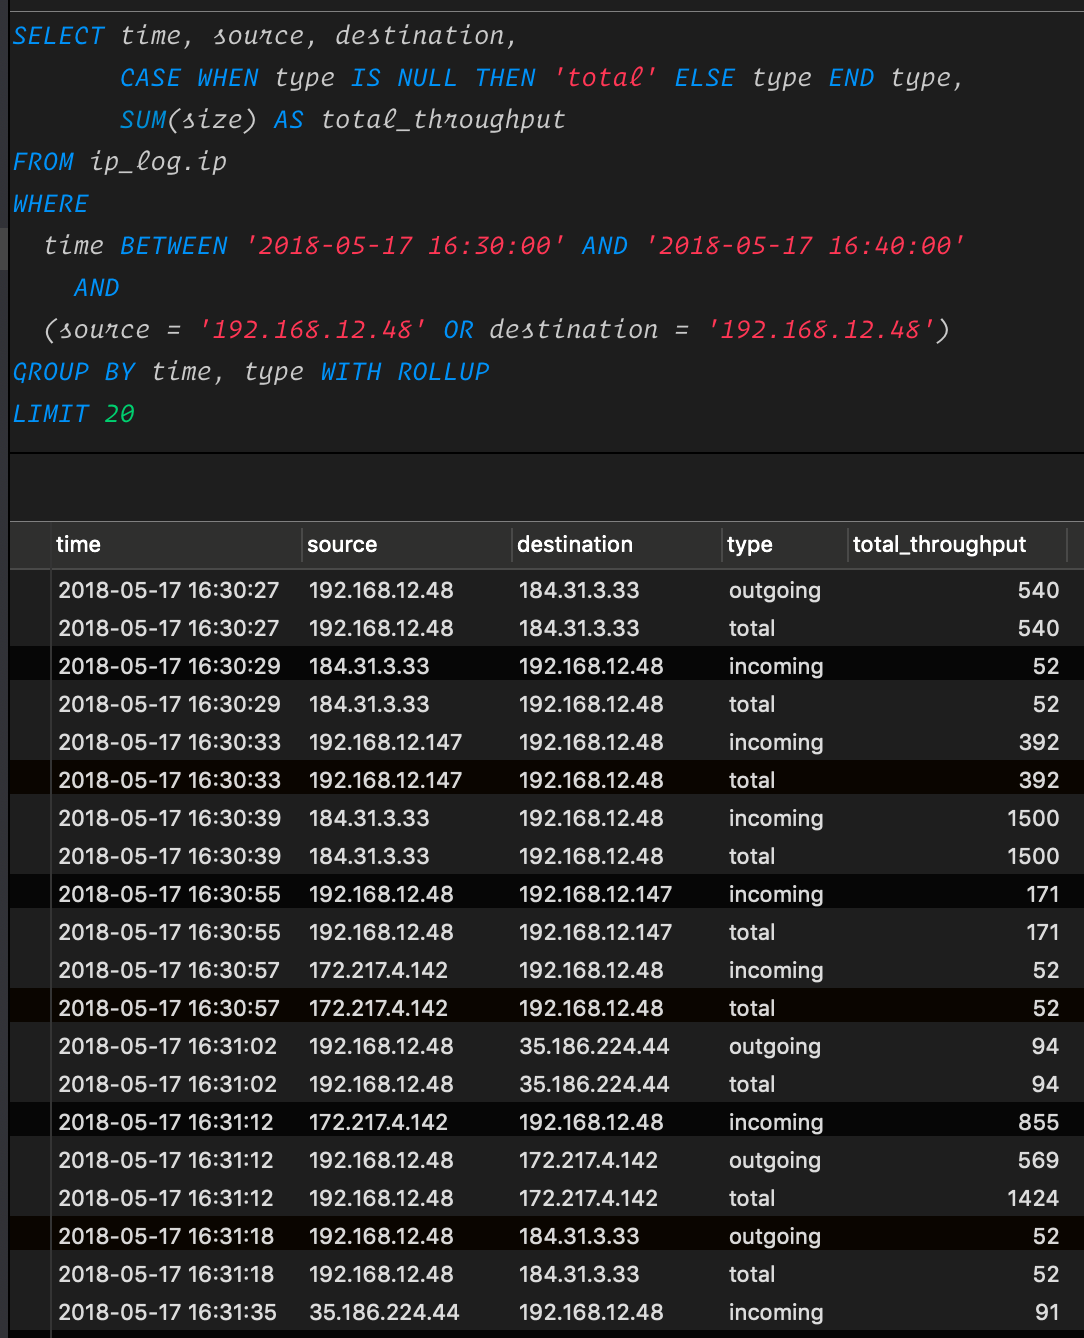
\includegraphics[width=1\textwidth]{figures/navicatRollup.png}
    \caption{Navicat IP query with rollup.}
    \label{fig:navicatRollup}
\end{figure}

The hex dump column drastically increases the size of each entry in the network table. However, as a raw network packet, it is very flexible and can be manipulated for many more use cases than the targeted columns we have. This flexibility is useful for future research, that may require data we did not explicitly pull out for this project

In the database, each device can be tracked down by looking for the IP address of that device in the source or destination columns. However, note that during set up, we did not set up static IPs for these devices. Because of this, a single device can be under multiple IPs within the table. We ignored this issue until a query for a particular IP stopped working. At which point we would invoke a command on the device whose IP changed to flood the database with packets from that device, query the database in the time frame of the command, and obtain the new IP. We logged all devices and their current IP in a Google Sheets \cite{googleSheets} file covered in subsection\ref{Device Inventory}.

\subsubsection{Power Table}

The power table holds the most important data for this portion of the research, and we refer to it for the majority of the paper's findings. The size of this table is much smaller than the network table. It contains 5.84 GB of data and 61,240,189 entries in the database. The significant difference in size between the IP table and power table is because each device only produces one entry power entry every second. The columns of the power table are shown below in figure\ref{tab:powcol}.

\begin{table}[H]
    \centering
    \caption{Columns in Power Table}
    \begin{tabular}{@{}lll@{}}
    \toprule
    Column Number & Column Name     & Data Type \\ \midrule
    1             & name            & varchar   \\
    2             & power\_mw       & int       \\
    3             & time            & datetime  \\
    4             & today\_kwh      & varchar   \\
    5             & on\_for         & varchar   \\
    6             & today\_on\_time & varchar
    \end{tabular}
    \label{tab:powcol}
    \end{table}

When working with this database, we generally query for a range of power packets in a given time range. We do this for either all devices, a subset of devices, or a single device. Some of the commands and results are shown below in figures \ref{fig:navicatPowerQuery} and \ref{fig:navicatNetworkQuery}.

\begin{figure}[H]
    \centering
    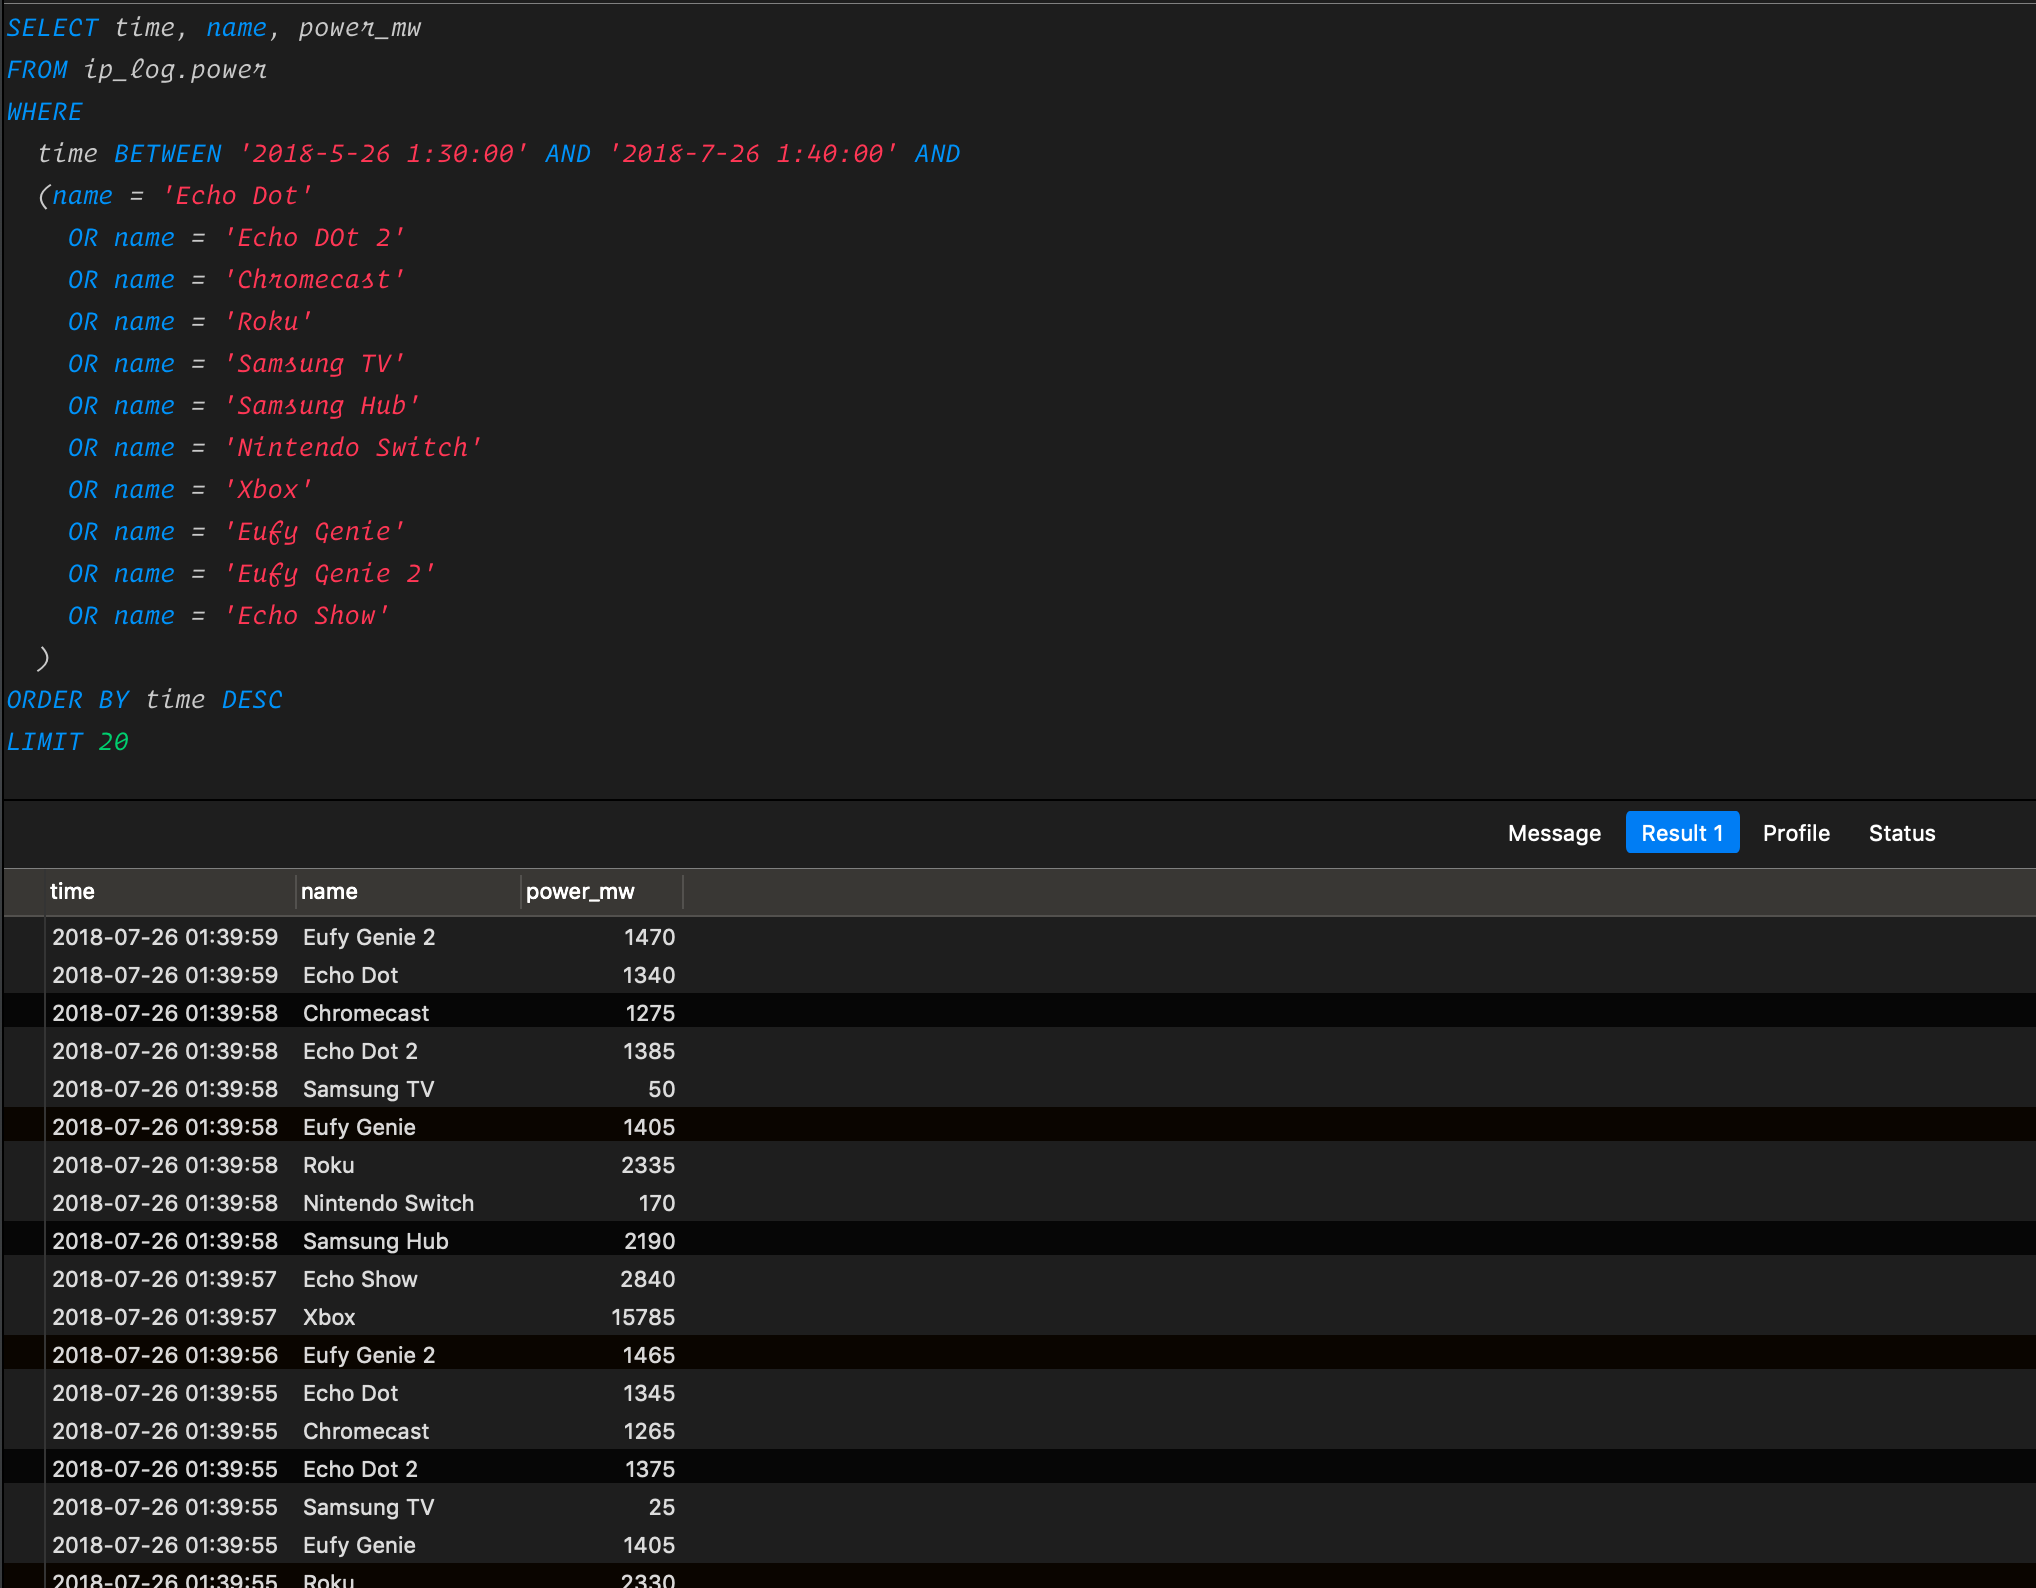
\includegraphics[width=1\textwidth]{figures/navicatPowerQuery.png}
    \caption{Power query from database with Navicat.}
    \label{fig:navicatPowerQuery}
\end{figure}

\begin{figure}[H]
    \centering
    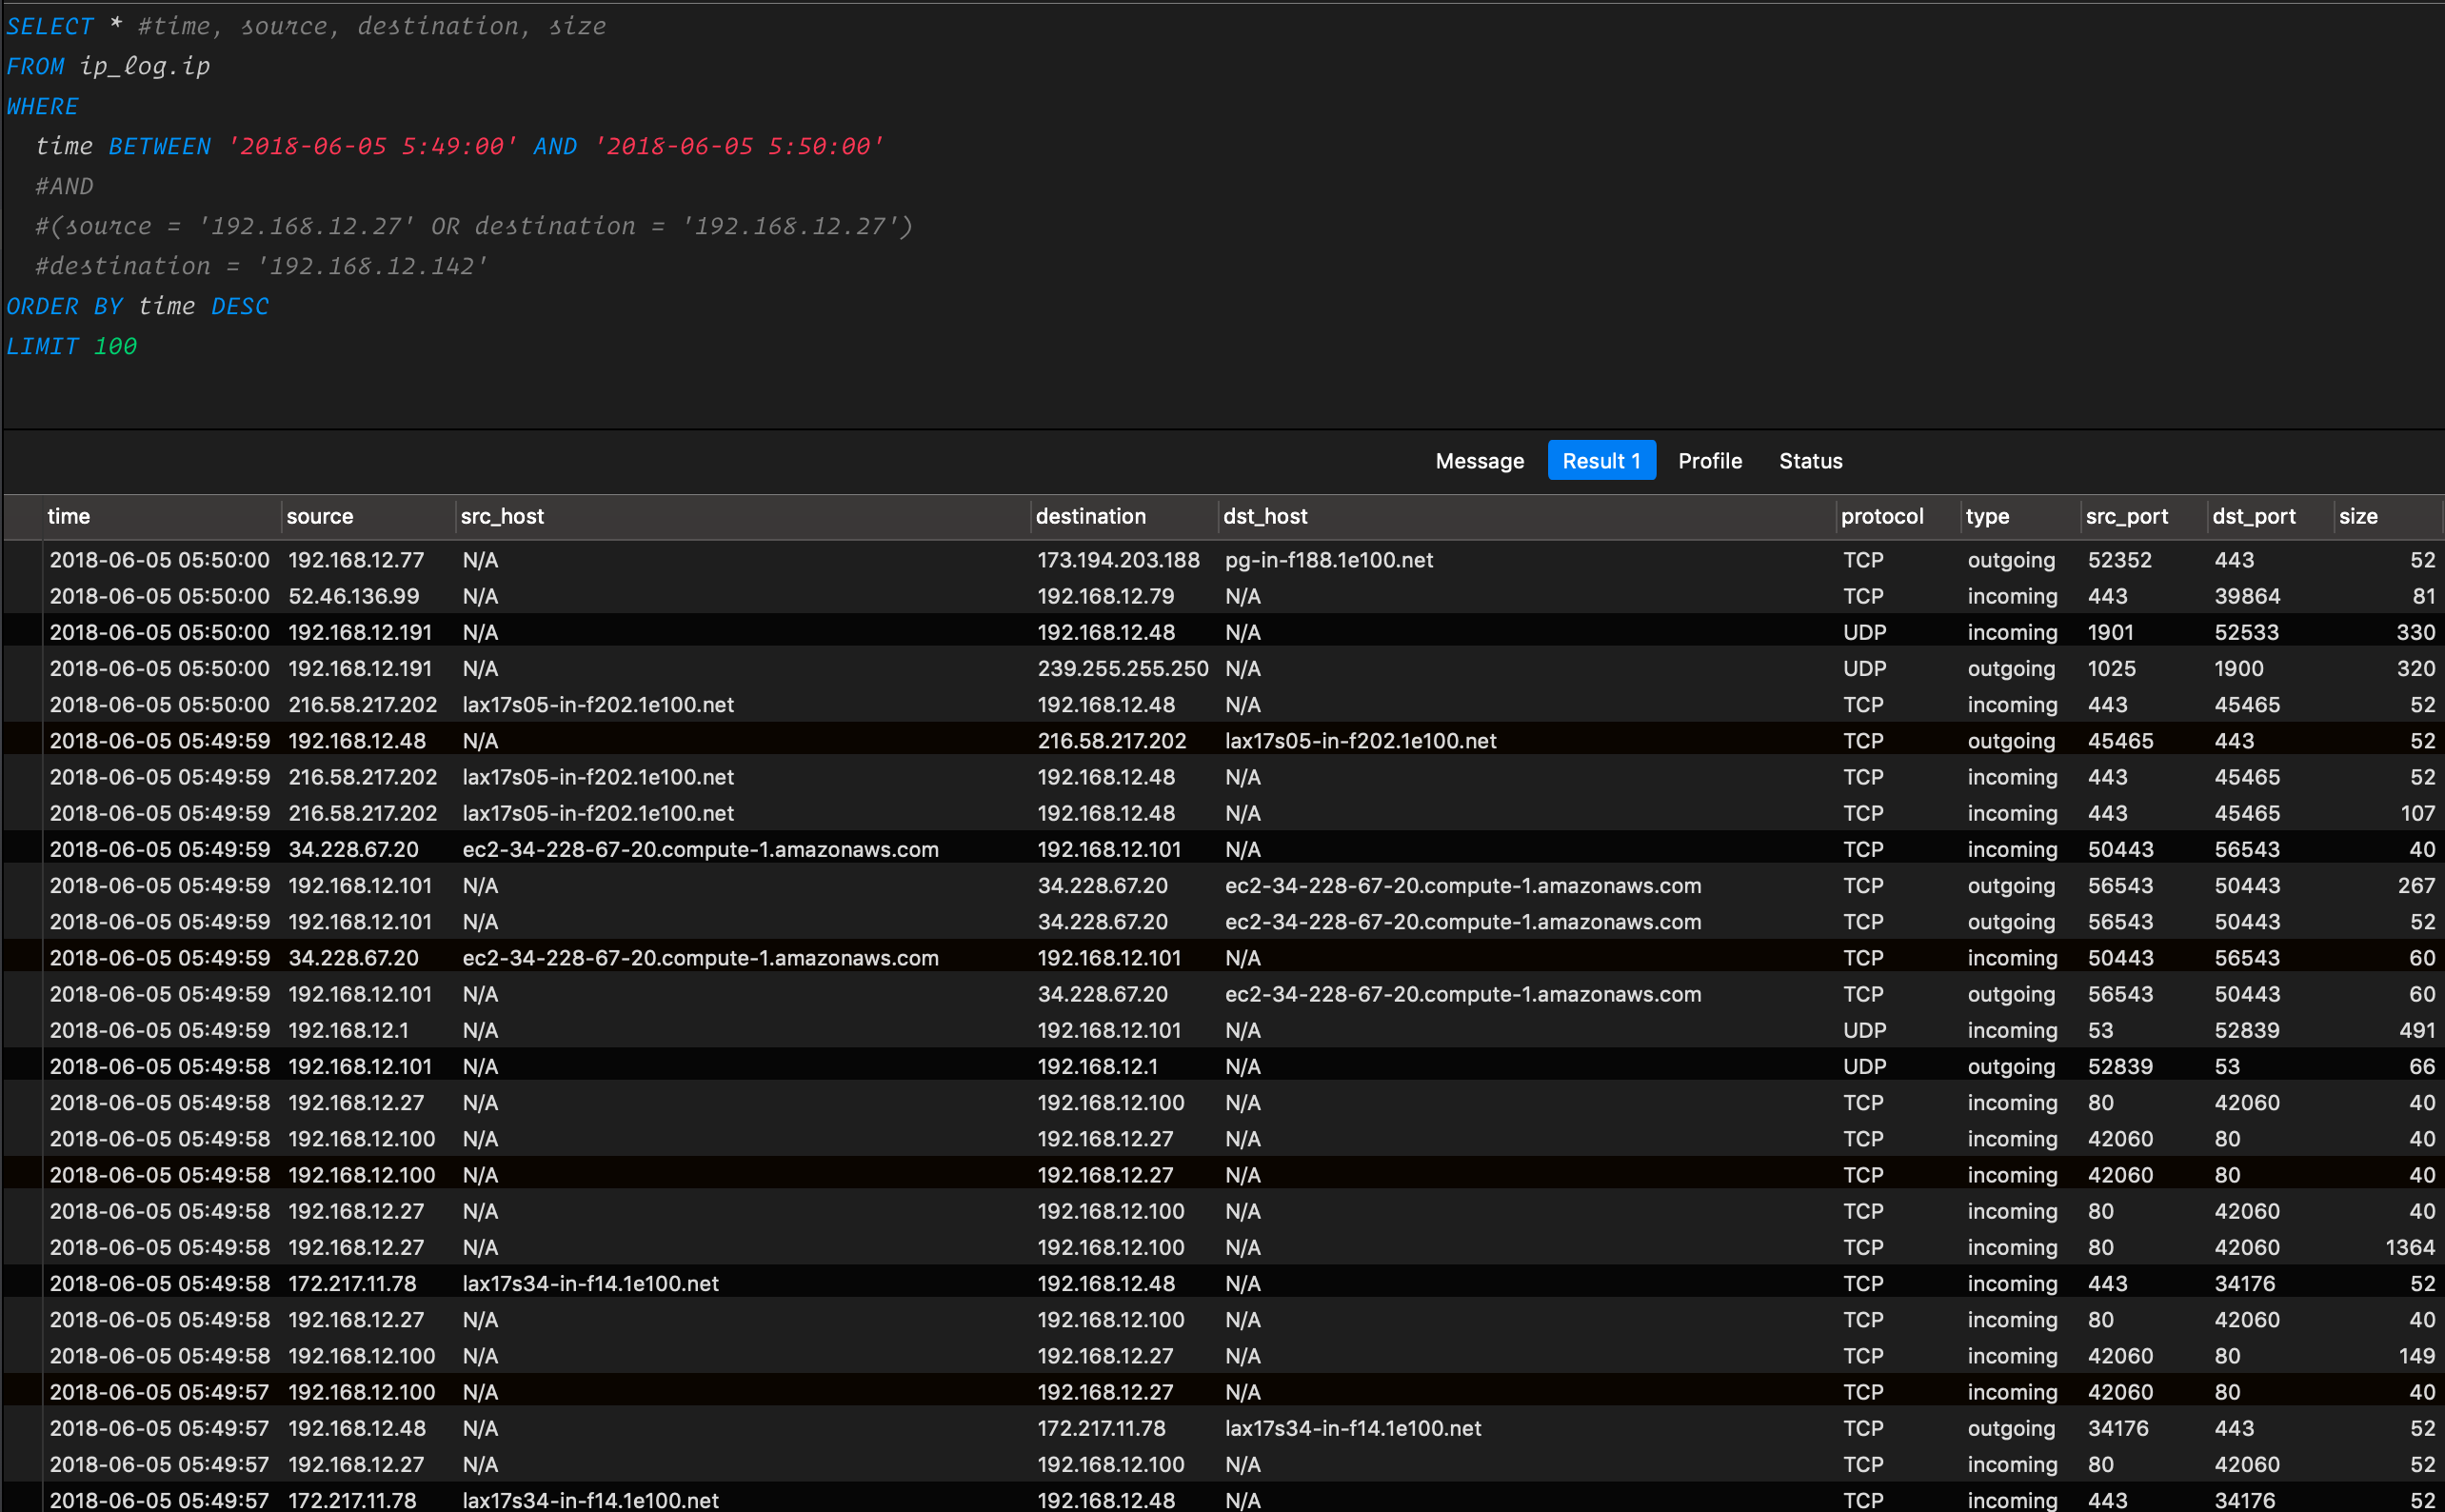
\includegraphics[width=1\textwidth]{figures/navicatNetworkQuery.png}
    \caption{Network query from database with Navicat.}
    \label{fig:navicatNetworkQuery}
\end{figure}
Within the power table, the name field is extracted from the name of the WeMo, which we manually name through the app. This can cause issues if the wrong device is connected to a WeMo. For example, the Echo Dot could have accidentally been connected to the WeMo named Google Home. There is no way to check for this besides manual examination, which we did after a few weeks, resetting all devices and causing a temporary void in power data. When we reset all devices, we also renamed some of the WeMos. For example, we changed ``echoDot'' to ``Echo Dot''. This way, all devices would follow the naming convention of separating words with spaces and capitalizing each word. Another possible naming convention could have been to name the WeMo by the IPs of the devices they connect to, but they are not static.

The sampling frequency for the power table is also low and missing some points. The script to query power data is not consistent and is unable to get power data at every second. To handle missing points, I interpolate them as shown in subsection \ref{realtimeIoTGrapher.py}. The interpolation process may introduce imprecise data as it fills a missing data point by extrapolating a linear path from the closest points before and after it.

\subsection{Device Inventory}
\label{Device Inventory}
To keep track of all devices and important details about them, we log a device's service, distributor, related email, IP address, dependencies, previous usage, and password into a Google Sheets file. An example of entries into the Device Inventory are shown below in table \ref{tab:deviceInventory}. The service field denotes the service a device provides, for example, the Google Home is a smart speaker. The device field denotes the specific manufacturer and device name. The Email and password fields denotes the email and password used when setting up the device. Some devices such as the Nintendo Switch were setup without an account. The IP address field denotes the IP address of the device within our local network. The dependencies field denotes anything the device is connected to or uses. For example, the Roku express is connected to a WeMo for power logging and comes with a controller for use. The used flag denotes whether the device was previously used or not, at which point, we could not log first time startup data for that device.

\begin{table}[H]
    \centering
    \caption{Device inventory excerpt. Password column not shown.}
    \resizebox{\linewidth}{!}{%
    \begin{tabular}{@{}lllllll@{}}
        \toprule
        Service      & Device            & Email                       & IP Address     & Dependencies     & Used \\ \midrule
        Speaker      & Amazon Echo Dot 1 & amazonEchoDotSS0@aol.com    & 192.168.12.79  & WeMo             & yes  \\
        Speaker      & Google Home       & googleHomeMiniSS0@aol.com   & 192.168.12.48  & WeMo             & no   \\
        Streaming    & Google Chromecast & googleChromecastSD0@aol.com & 192.168.12.78  & WeMo             & no   \\
        Streaming    & Roku Express      & rokuExpressSD0@aol.com      & 192.168.12.68  & WeMo, controller & no   \\
        Game Console & Nintendo Switch   & n/a                         & 192.168.12.160 & WeMo, controller & no   \\ \bottomrule
        \end{tabular}}
    \label{tab:deviceInventory}
\end{table}


\subsection{Usage Flow}

One of the goals of this work is to create a data set that represents the baseline of normal network traffic and power usage. To do this, we used each IoT device at least twice a week for the year length of this research. To build a proper dataset that other people could use for research, we set up a list of things that we should do for each device interfacing with it. We logged the activities into Google Sheets so that these events could be correlated to entries in the database, giving context when looking back on this data. For example, if someone were to look at the database and notice that the power and network traffic was high for 3 minutes, they could look at our logs and see that the device was streaming music for those 3 minutes and assume that it was normal usage.

When logging events into Google Sheets, we include the start, end time, name of the device(s), action performed, and any individual notes. When naming the devices, we used the same naming as we did for the WeMos to maintain consistency from the log to the database. An example of entries into the table is shown in Table \ref{tab:events}.

\begin{table}[H]
    \centering
    \caption{Event Log Excerpt}
    \begin{tabular}{@{}lllll@{}}
        \toprule
        Date & Start Time & End Time & Device & Event \\ \midrule
        5/25/2018 & 12:44:42 & 12:47:04 & Home Mini & Ask for news \\
        5/25/2018 & 12:55:07 & 12:56:37 & Echo Dot & Ask for news \\
        5/25/2018 & 12:55:57 & 12:56:17 & Echo Show & Ask for weather \\
        5/25/2018 & 12:56:44 & 13:03:07 & Home Mini & Play music \\ \bottomrule
        \end{tabular}
    \label{tab:events}
\end{table}

The following subsections explains the script created to automate the event logging portion of the research. Then it explains the specific procedure we ran each group of IoT devices through whenever we interfaced with them.

\subsubsection{Google Sheets Script}

Logging information into the spreadsheet is a tedious task, especially when trying to analyze each device while running tasks on them. The code for the script is shown below in Listing~\ref{lst:sheetScript}.

\noindent
\begin{minipage}{\textwidth}
\begin{lstlisting}[basicstyle=\linespread{0.95}\ttfamily, language=C,label={lst:sheetScript},caption={Open and Read from a Socket}]
function onEdit() {
  var s = SpreadsheetApp.getActiveSpreadsheet().getSheetByName("Event Log");
  var r = s.getActiveCell();
  var c = r.getColumn();

  if( c == 4 || c == 5) { // checks the column
    var dateCell = r.offset(0, -3);

    if( dateCell.getValue() === '' ) {// is empty?
      var startTimeCell = r.offset(0, -2);

      // fill in the start time and date
      var date = new Date();
      dateCell.setValue(date);
      startTimeCell.setValue(date.toLocaleTimeString());
    }
  }

  if( c == 6 ) { // checks that the description is being entered
    // if so fill in the end time
    var endTimeCell = r.offset(0, -3);

    if ( endTimeCell.getValue() === '' ) {
      endTimeCell.setValue(new Date().toLocaleTimeString());
    }
  }
}
\end{lstlisting}
\end{minipage}

\subsubsection{Smart Speakers}

Whenever interfacing with these devices, we always queried for the weather and the news. The specific phrases we used ``$<$wake word$>$ what's the weather'' and ``$<$wake word$>$ what's the news'', we  set a reminder for a random task in a random timeframe, and we muted the devices for a few minutes to see if they were still listening if we said the wake word.

\subsubsection{Video Game Consoles}

When interfacing with these devices, we played a game on the device for at least 15 minutes. Every week, we also browsed for games on the game store and downloaded free demos.

Afterward, we would turn off the Xbox and put the Nintendo Switch into sleep mode. The Nintendo Switch could not be put to sleep when docked, only when disconnected from the dock, so it was set to sleep rather than power off.

\subsubsection{Streaming Devices}

Within the Media Players section, we include the Roku Express, Chromecast, Amazon Firestick, and Samsung Smart TV. When interfacing with these devices, we watched YouTube for at least either one video or 3 minutes.

For the Chromecast, we cycled through different devices to cast videos from, including the iPad and the Chromebook. We wanted to get varied data in case the Chromecast prioritized streaming from different devices.

\subsubsection{Tablets}
In this experimental setup, we used the tablets less for investigative purposes, but more to set up and interface with other devices.

However, we still tracked the data and had a small set list of things to do on these devices. We used each tablet to browse the web, watch YouTube, and use various apps.

\subsubsection{Security Camera}

The only security camera we worked with was the Eray Security Camera.

Whenever interfacing with this device, we used the device under the app NVAS2 in the iPad for at least 2 minutes. Usage included streaming video from the camera to iPad and viewing it. We also controlled the camera through the app with pan and tilt commands. When done experimenting with the security camera, we disconnected the tablet from the camera by using the ``end stream'' button in the NVAS2 app.

\subsection{realtimeIoTGrapher.py}
\label{realtimeIoTGrapher.py}

This section covers a visual tool I created to look for trends. We initially graphed the data into Google Sheets and graphed it. The tables and formulas are shown in figure \ref{fig:excelLogging}. This process was tedious and time-consuming. We had to copy the data over after making a SQL query, extract unique time values, and then get the total network and power usage at each time interval.

To address these problems, I created a python script that automatically forms graphs, including the one shown in figure \ref{fig:interpolated} when given the time range and the devices. This automation sped up the analysis process and provided extra features covered in section \ref{Features}.

This Python script leverages the Plotly library, which, given data, will graph it onto a local web page for viewing. Plotly comes with many useful tools for further analysis and can be extended to run on a public web page for public viewing.

I plan to distribute this out with our database so that researchers can view the power and network information of any device at a glance.

\begin{figure}[H]
    \centering
    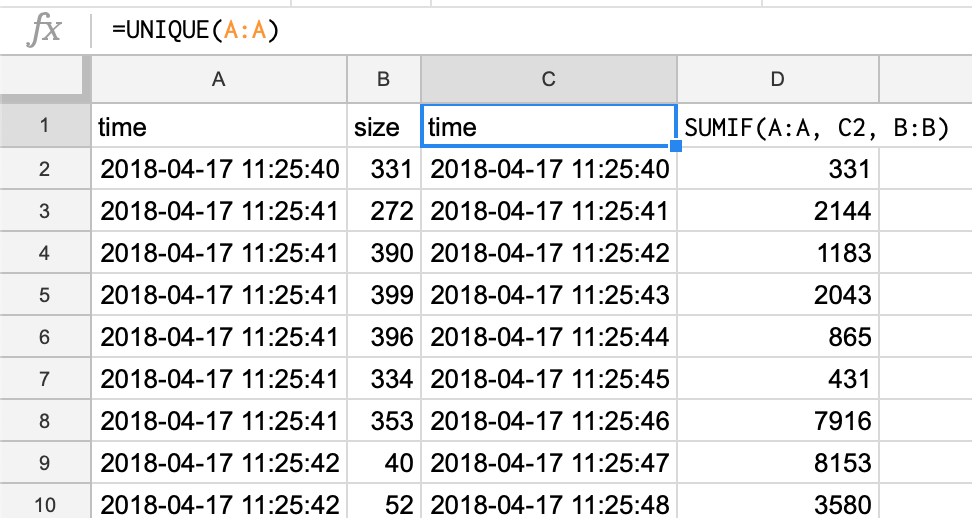
\includegraphics[width=1\textwidth]{excelLogging}
    \caption{Manual Analysis of IoT devices in Google Sheets: Raw data shown in columns A and B are then formatted into columns C and D for Graphing}
    \label{fig:excelLogging}
\end{figure}

\begin{figure}[H]
    \centering
    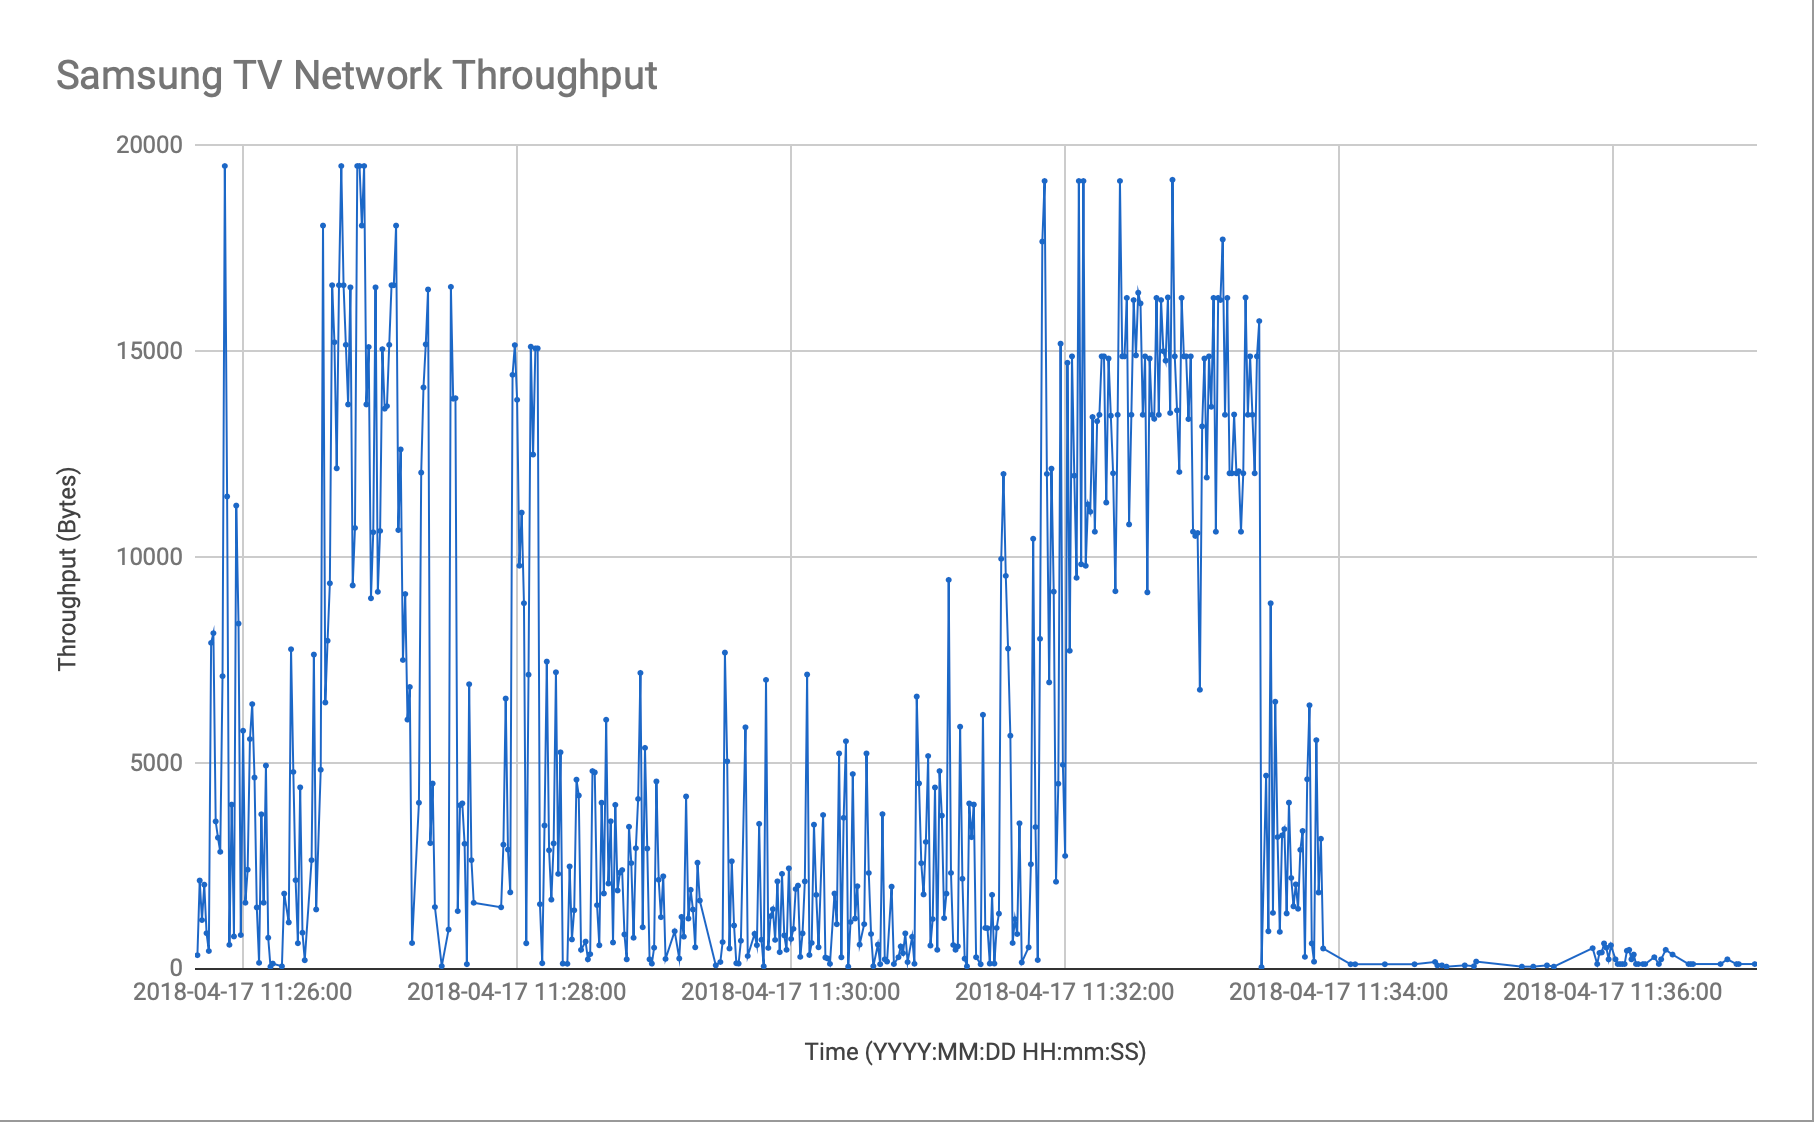
\includegraphics[width=1\textwidth]{figures/tvThroughput.png}
    \caption{Resulting graph of dataset shown in Figure \ref{fig:excelLogging}}
    \label{fig:tvThroughput}
\end{figure}

\subsubsection{Features}
\label{Features}

This section discusses the features that RealTimeIoTGrapher (grapher) provides.

At its core, this program automates the creation of the graph shown in figure \ref{fig:tvThroughput}. The user can specify a time range that the graph should cover and what devices to graph. By default, the graph shows power, input traffic, output traffic, and total network traffic over the time range specified.

The grapher also annotates the data by including a line denoting the average for each of the traces over the time range currently displayed. It also annotates the maximum and minimum values in the time range for each trace. The grapher can also display information in real time for a user settable interval amount of time, updating every second.

The Plotly libraries also provide useful tools when displaying these IoT graphs. It is possible to zoom in and out the displayed graph, select specific traces for viewing, save the graph, and hover over data points to display the specific value. Finally, once a graph is saved Plotly allows further editing of the graph so that it is formatted the way the user wants.

\noindent
\begin{minipage}{\textwidth}
    \begin{lstlisting}[language=SQL, label={lst:rollup},caption={Efficient SQL query to obtain total Network throughput at each second.}]
    def throughput_query_in_range(db_connection, device, start_time, end_time):
    sql_query = """
        SELECT
            time,
            CASE WHEN type IS NULL THEN 'total' ELSE type END type,
            SUM(size) AS total_throughput
        FROM ip_log.ip
        WHERE
            time BETWEEN '%s' AND '%s' AND
            (source = '%s' OR destination = '%s')
        GROUP BY time, type WITH ROLLUP;
    """ % (start_time, end_time, ip[device], ip[device])

    dataframe = pd.read_sql_query(sql_query, db_connection)

    return dataframe
    \end{lstlisting}
\end{minipage}

To reduce local computation, the grapher offloads work to the server through a SQL query. When querying for network data, it performs a SQL ROLLUP to sum the incoming and outgoing network throughput to obtain the total throughput. ROLLUP is required because it provides nested queries and causes the query to sum up the data by time for each type of packet. This query is formatted as shown in listing \ref{lst:rollup}.

\begin{figure}[H]
    \centering
    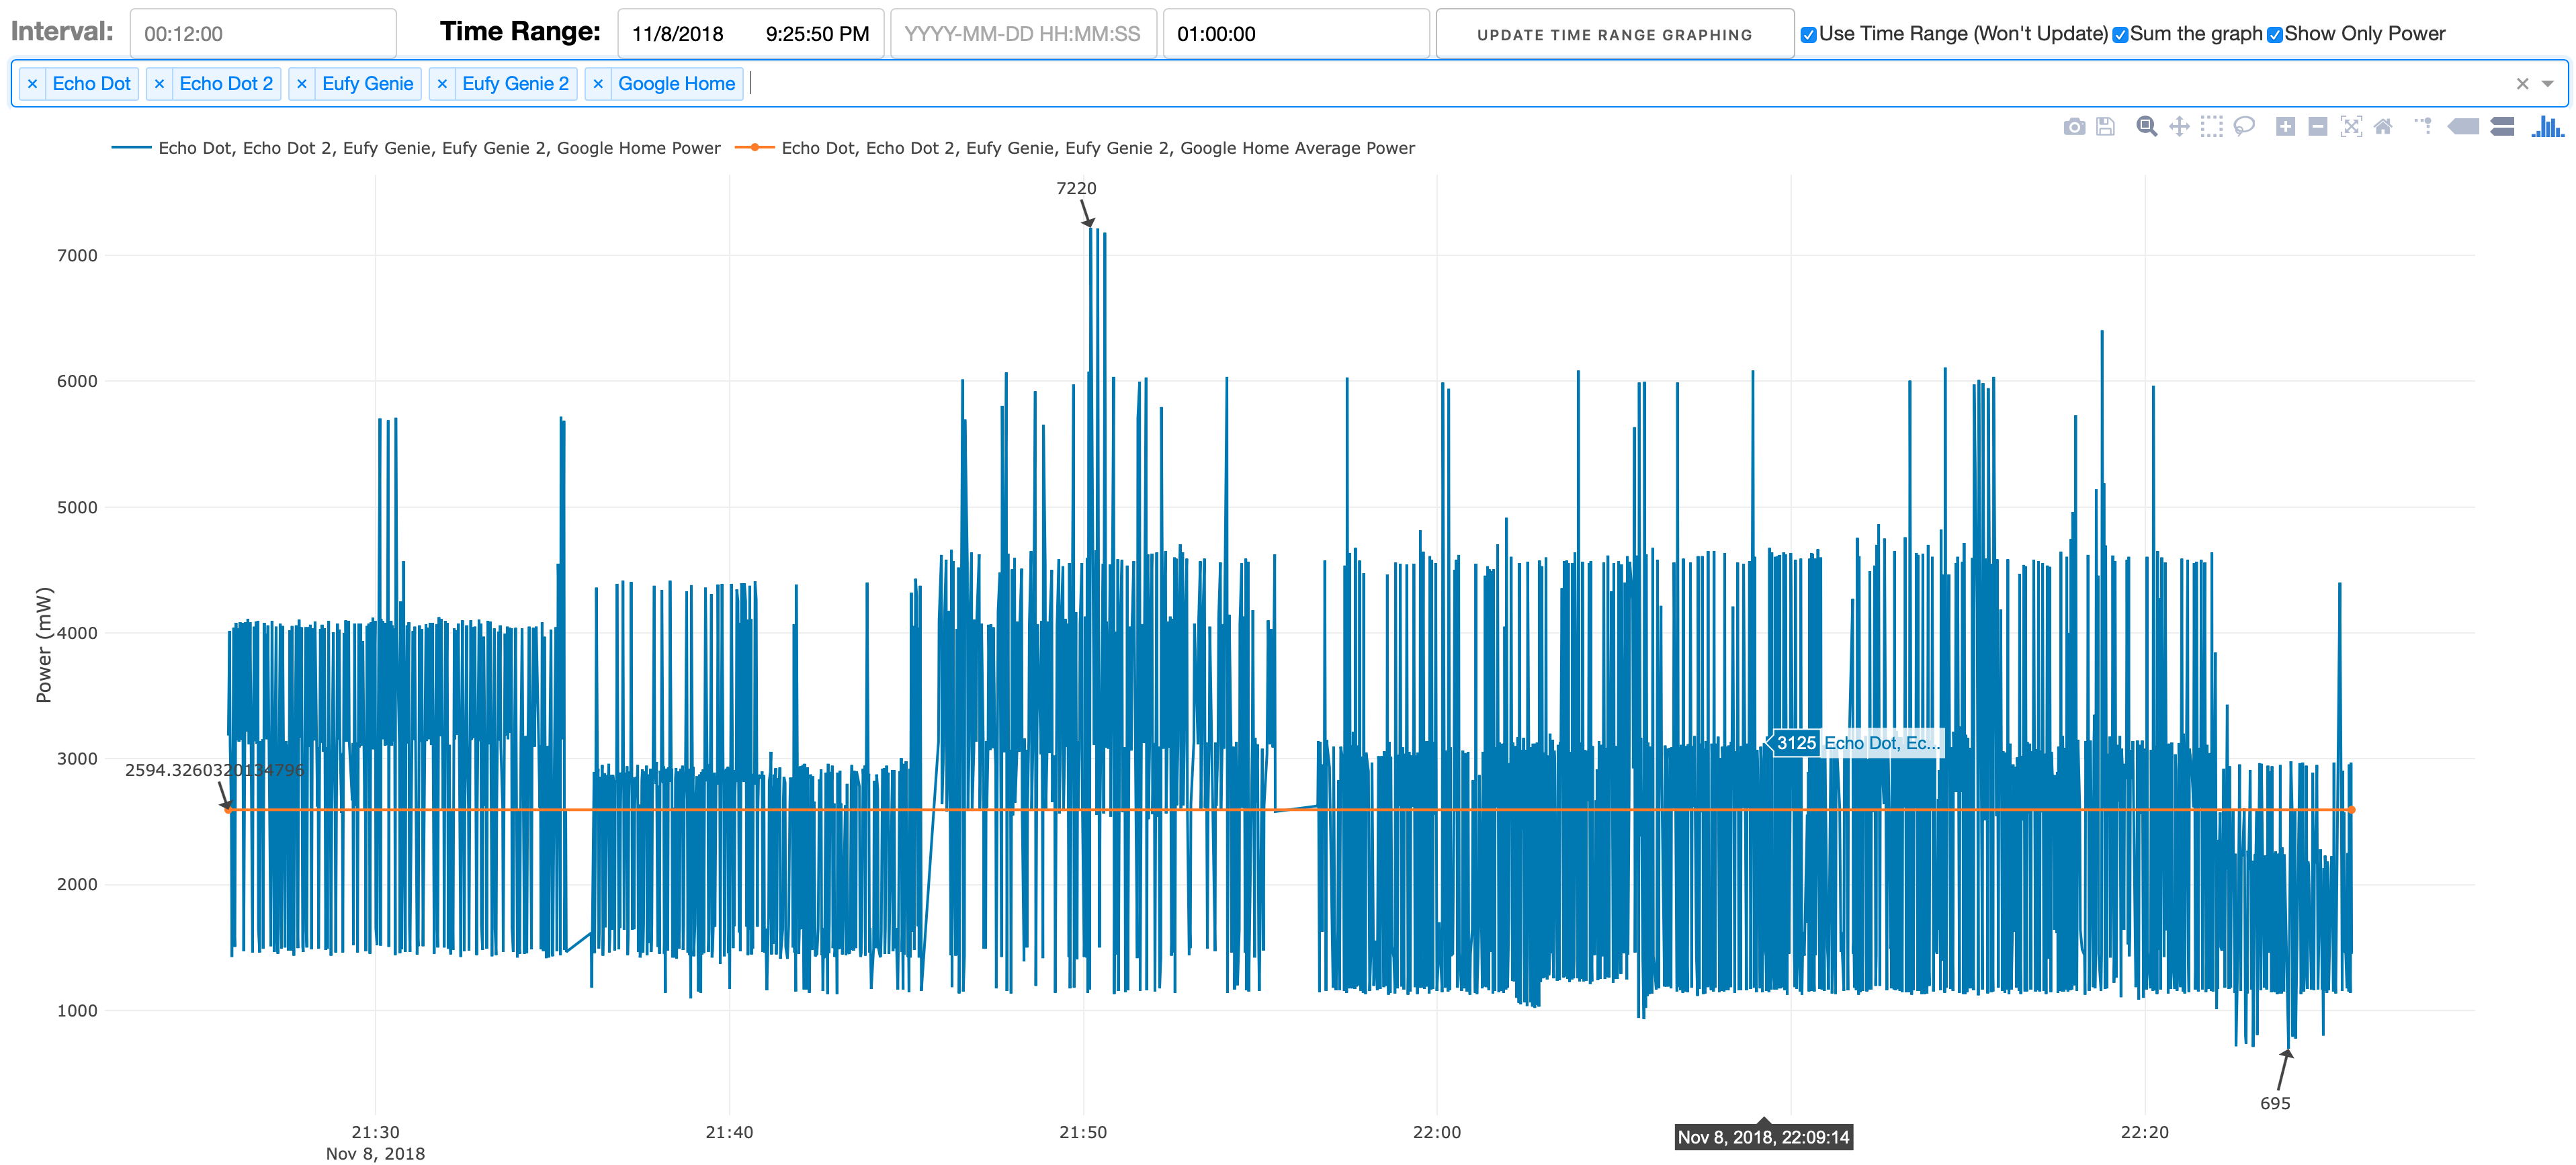
\includegraphics[width=1\textwidth]{figures/noninterpolated.png}
    \caption{Summed power traces without interpolation.}
    \label{fig:noninterpolated}
\end{figure}

\begin{figure}[H]
    \centering
    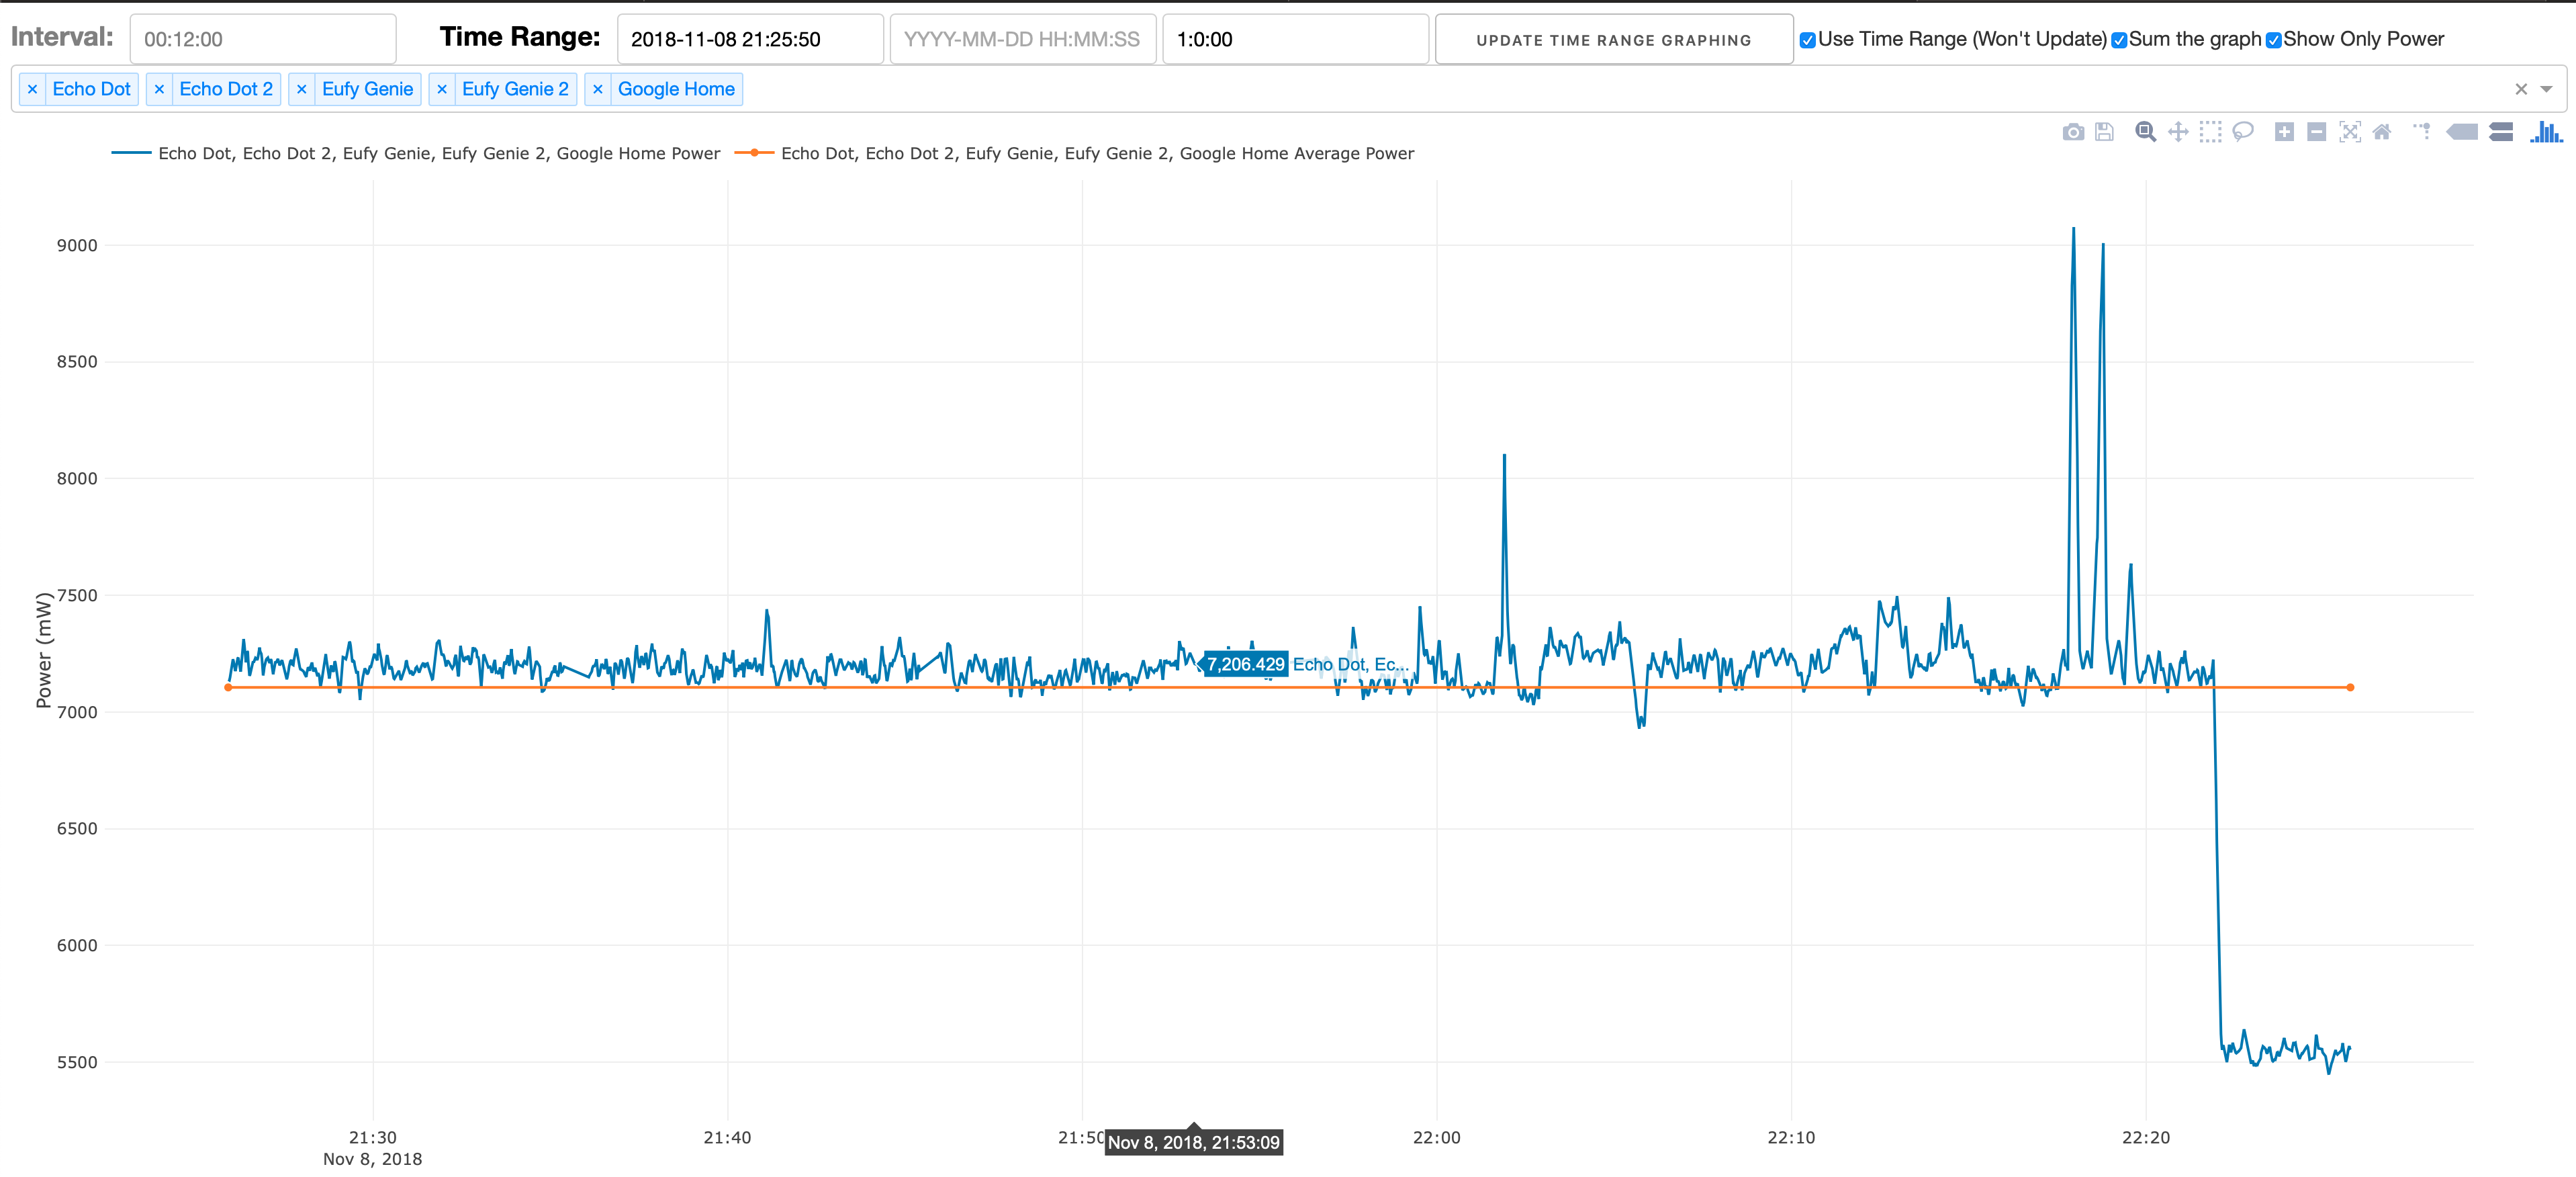
\includegraphics[width=1\textwidth]{figures/interpolated.png}
    \caption{Summed power traces with interpolation.}
    \label{fig:interpolated}
\end{figure}

The grapher can also sum up all power traces into one single trace. Originally, when summing the graphs, it would add the two Pandas \cite{pandas} data frames that represent each trace, and graph the result, shown in figure \ref{fig:noninterpolated}. Pandas is a Python library that represents a multidimensional array as a table, providing useful methods for manipulating the dataset. However, the WeMo does not always sample every second. This is an issue if, at time, one device X has a power point, but another device does not. The summation will count the empty data point as 0, resulting in an erroneous sum. This was solved by interpolating data for every second for each device before summing data frames, with a built-in Pandas feature. Interpolation is shown in \ref{fig:interpolated} as a graph.

\subsubsection{Visual Takeaway}
This tool created most of the images shown in section \ref{Results}. A few other researchers such as Frawley's have used this tool for data visualization. The grapher provides real-time or historical graphs on any in the database device for individual analysis or comparison with little effort or time. Additional features from Plotly also provides an easy way to format graphs for presentations or papers.

The summation feature can simplify the graph and provide a more holistic view of power usage, making it easier to spot patterns. In this paper, the summation feature is used to simulate the concept of a household's ``powerline'' where all energy usage would be summed up into one power meter.

\subsubsection{Limitations}
As this tool was created entirely for research purposes, there are some edge cases that it fails to handle.

When the database has too many connections, the software will refuse to connect, and the grapher will not work. When graphing in real time, the grapher makes a new connection for each query. If a query fails, connections can quickly build up.

The graphing tool also slows as the time frame requested increases. We have noticed a slow down for queries with time frames longer than seven hours. In the static graphing mode, the tool slows down before graphing the information. However, in real time graphing mode, the tool will make many slow queries, eventually causing too many connections to the database and undefined behavior.

The graphing tool uses a lookup table that maps the IP address of the device to the corresponding name given to the WeMos. Because we manually create the lookup table, when any of these fields change, the graphing is not able to find the device. In some cases, this causes the graphing tool to crash. To solve this, the user must manually change the IP addresses defined in the lookup table in lines 23-39 shown in listing \ref{lst:ipLookup} below.

To figure out the new IP address for the table, the user must perform a SQL query in the time frame that a device is doing something, and manually examine the network traffic to see which IP has the highest network throughput. With this method, we had to ensure only one device was in use so that an IP address for another device would not be confused for the current device.

\begin{minipage}{\textwidth}
    \begin{lstlisting}[label={lst:ipLookup},caption={IP lookup table in real time IoT grapher.}]
    #region IP Addresses of all devices we are tracking
    ip = {
        'Chromecast':       '192.168.12.77',
        'Echo Dot 2':       '10.42.0.132',
        'Echo Dot':         '10.42.0.150',
        'Eufy Genie':       '10.42.0.223',
        'Eufy Genie 2':     '10.42.0.172',
        'Fire Stick':       '192.168.12.113',
        'Google Home':      '10.42.0.236',
        'IP Camera':        '192.168.12.58',
        'Nintendo Switch':  '192.168.12.160',
        'Roku':             '192.168.12.68',
        'Samsung Hub':      '192.168.12.100',
        'Samsung TV':       '192.168.12.191',
        'Smart Light':      '192.168.12.27',
        'Xbox':             '192.168.12.251',
        'Echo Show':        '192.168.12.122',
        'Appliance':        '192.168.12.122',
        'Appliance1':        '192.168.12.122',
    }
    \end{lstlisting}
\end{minipage}

\chapter{Results and Discussion}
\label{Results}
This chapter covers different network and power usage patterns for the IoT devices in the testbed. First, section \ref{swappingSwitch} informally compares the smart switches between devices to show that they are accurate for this research's purposes. Section \ref{wholeDB} covers the the percentage of each protocol in the database for an overall view of home IoT devices. Section \ref{General Analysis} covers smart speakers' and streaming devices' network and power use while idle, in use, and during first boot. Sections \ref{wholeDB} and \ref{General Analysis} serve as precursory analysis to fingerprint devices and give example usages of the database and visualizer tool.

After general analysis, section \ref{Power Analysis on Smart Speakers} shows how the presence of a user in their house and a smart device can be determined form power traces. This starts the focus of the research to use a shared power line (simulation for home power line) to visually determine what smart speaker is in use. Sections \ref{sumPowerGraph} and \ref{sumPowerGraphWithNoise} cover summed power graphs of the smart speakers with and without noise from high power household devices. Finally section \ref{smartSpeakerComparisonSection} ends with a comparison between smart speakers for further general analysis.

Within each section, after presenting the results, the paper discusses the implications of the data. The results and discussion presented are visual and informal, but strongly support the claims they make.

When obtaining data, most of the packets are encrypted, so the data presented focuses on metadata such as size, protocol, source IP, and dest IP. For power analysis, we focus on the power used at each second.

\section{Swapping the Power Switch}
\label{swappingSwitch}
To check if the smart switch voltage readings are accurate we swapped various devices with various power switches. Some examples are shown \ref{fig:swapEcho1Home}, \ref{fig:swapEufy1Echo1}, and \ref{fig:swapEufy1Home}. After swapping the switches, each device would take some time to start up, this time is highlighted by the colored box in figures \ref{fig:swapEcho1Home}, \ref{fig:swapEufy1Echo1}, and \ref{fig:swapEufy1Home}. I

In every case the traces swapped as we swapped the device connected to each smart switch. This informal sanity check confirmed accurate enough power switches for visual analysis.

\begin{figure}[H]
    \centering
    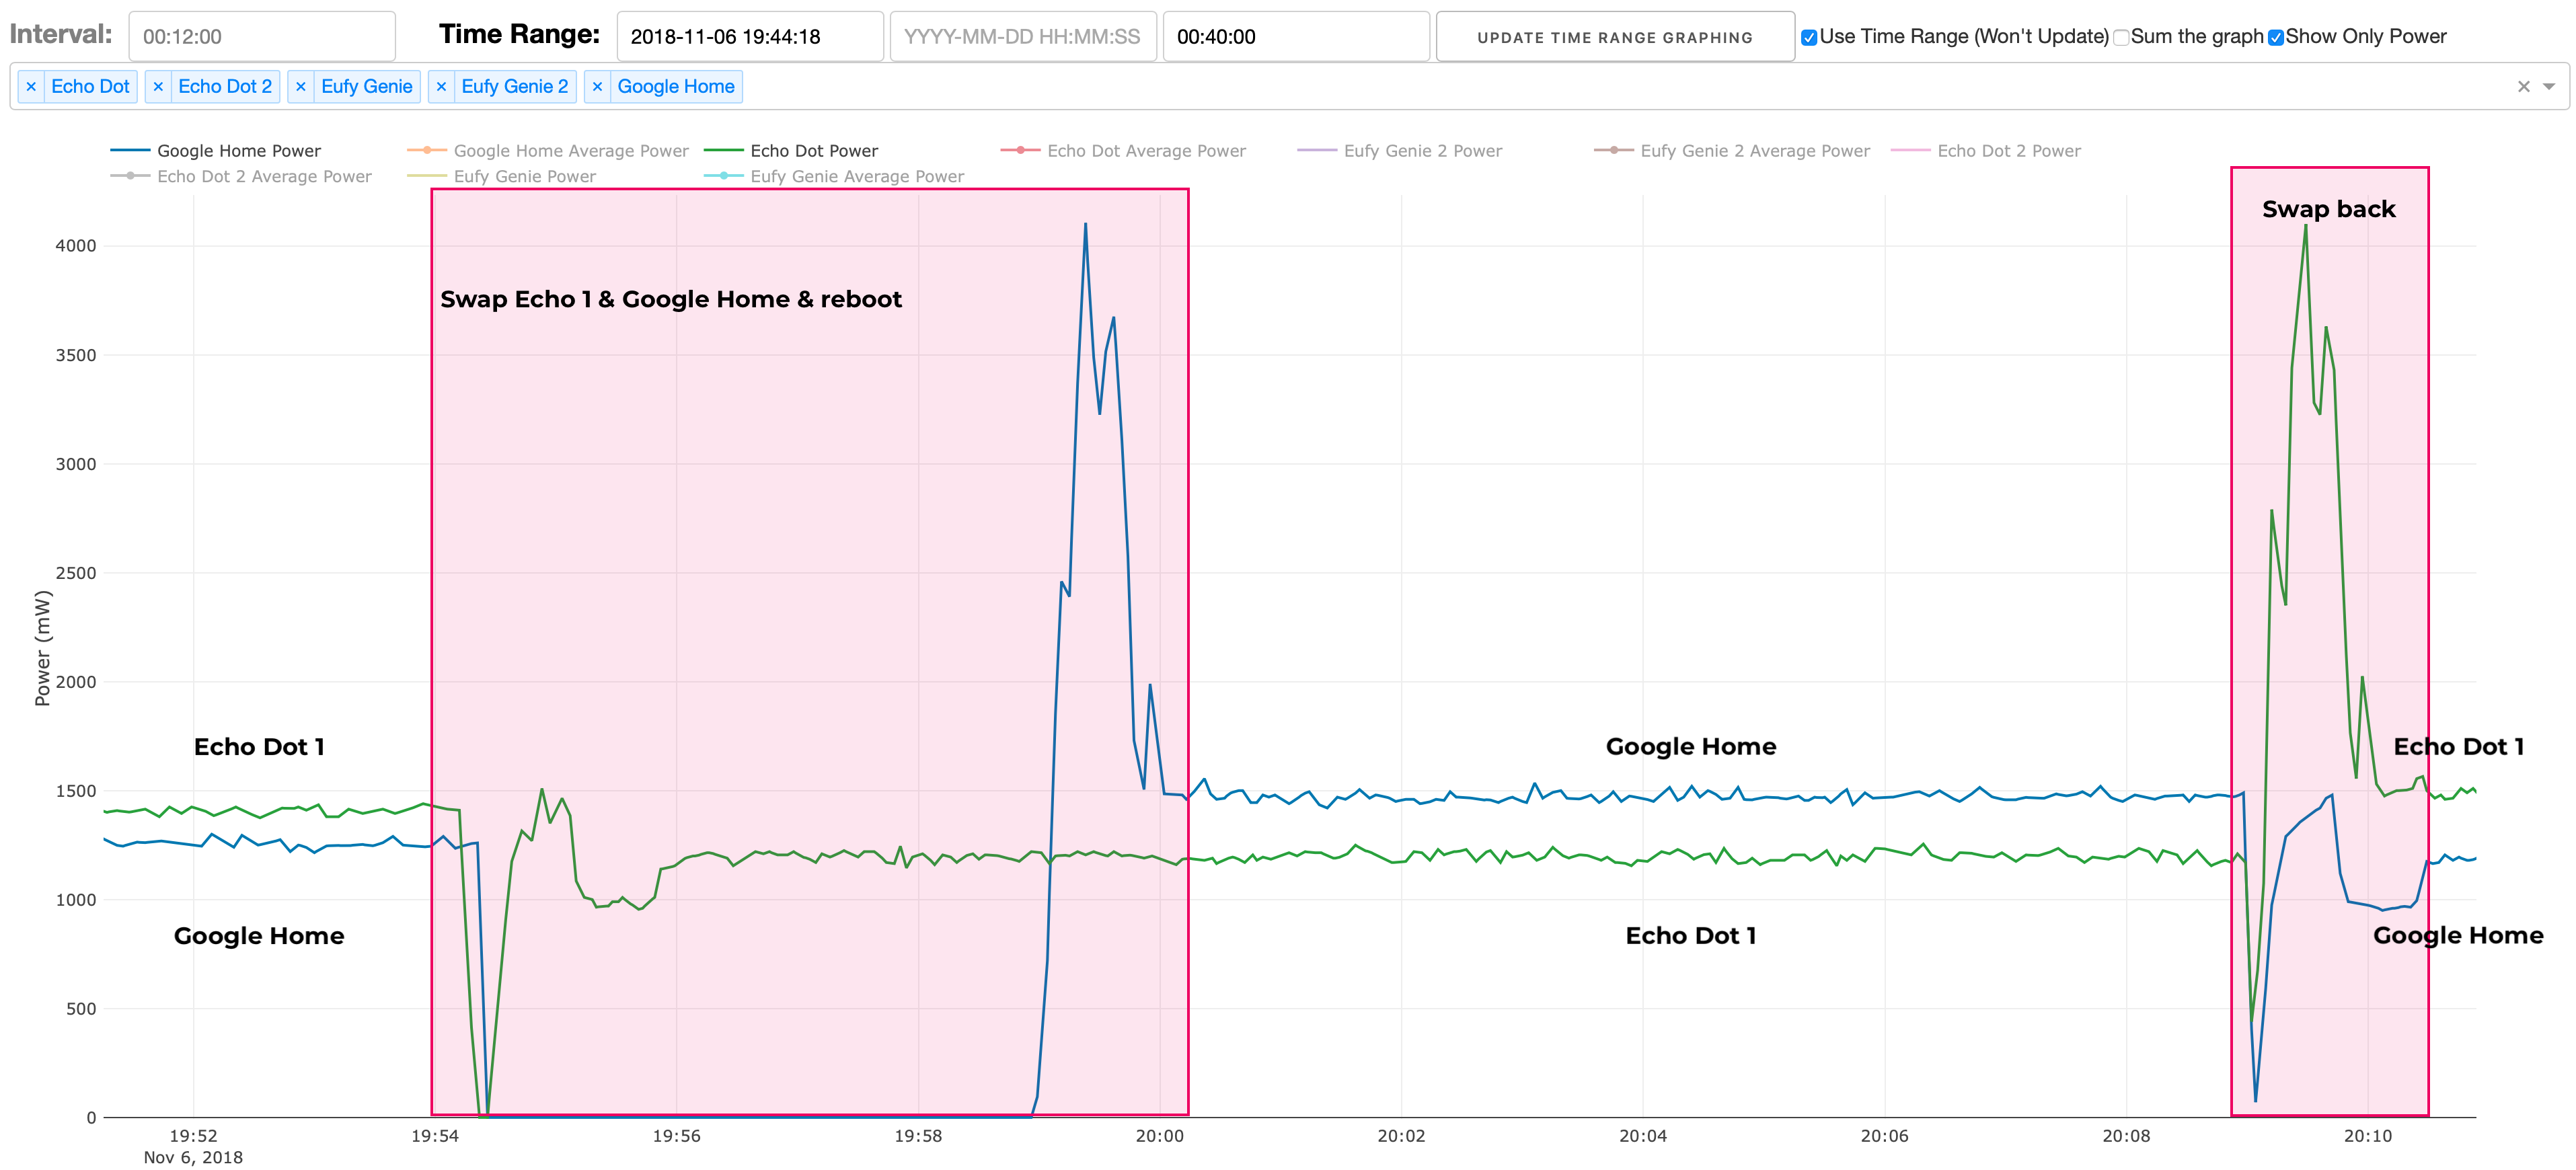
\includegraphics[width=1\textwidth]{figures/swapEcho1Home.png}
    \caption{Connected the Echo Dot 1 to WeMo for `Eufy Genie 1' and vice versa. The traces swap before and after switching.}
    \label{fig:swapEcho1Home}
\end{figure}

\begin{figure}[H]
    \centering
    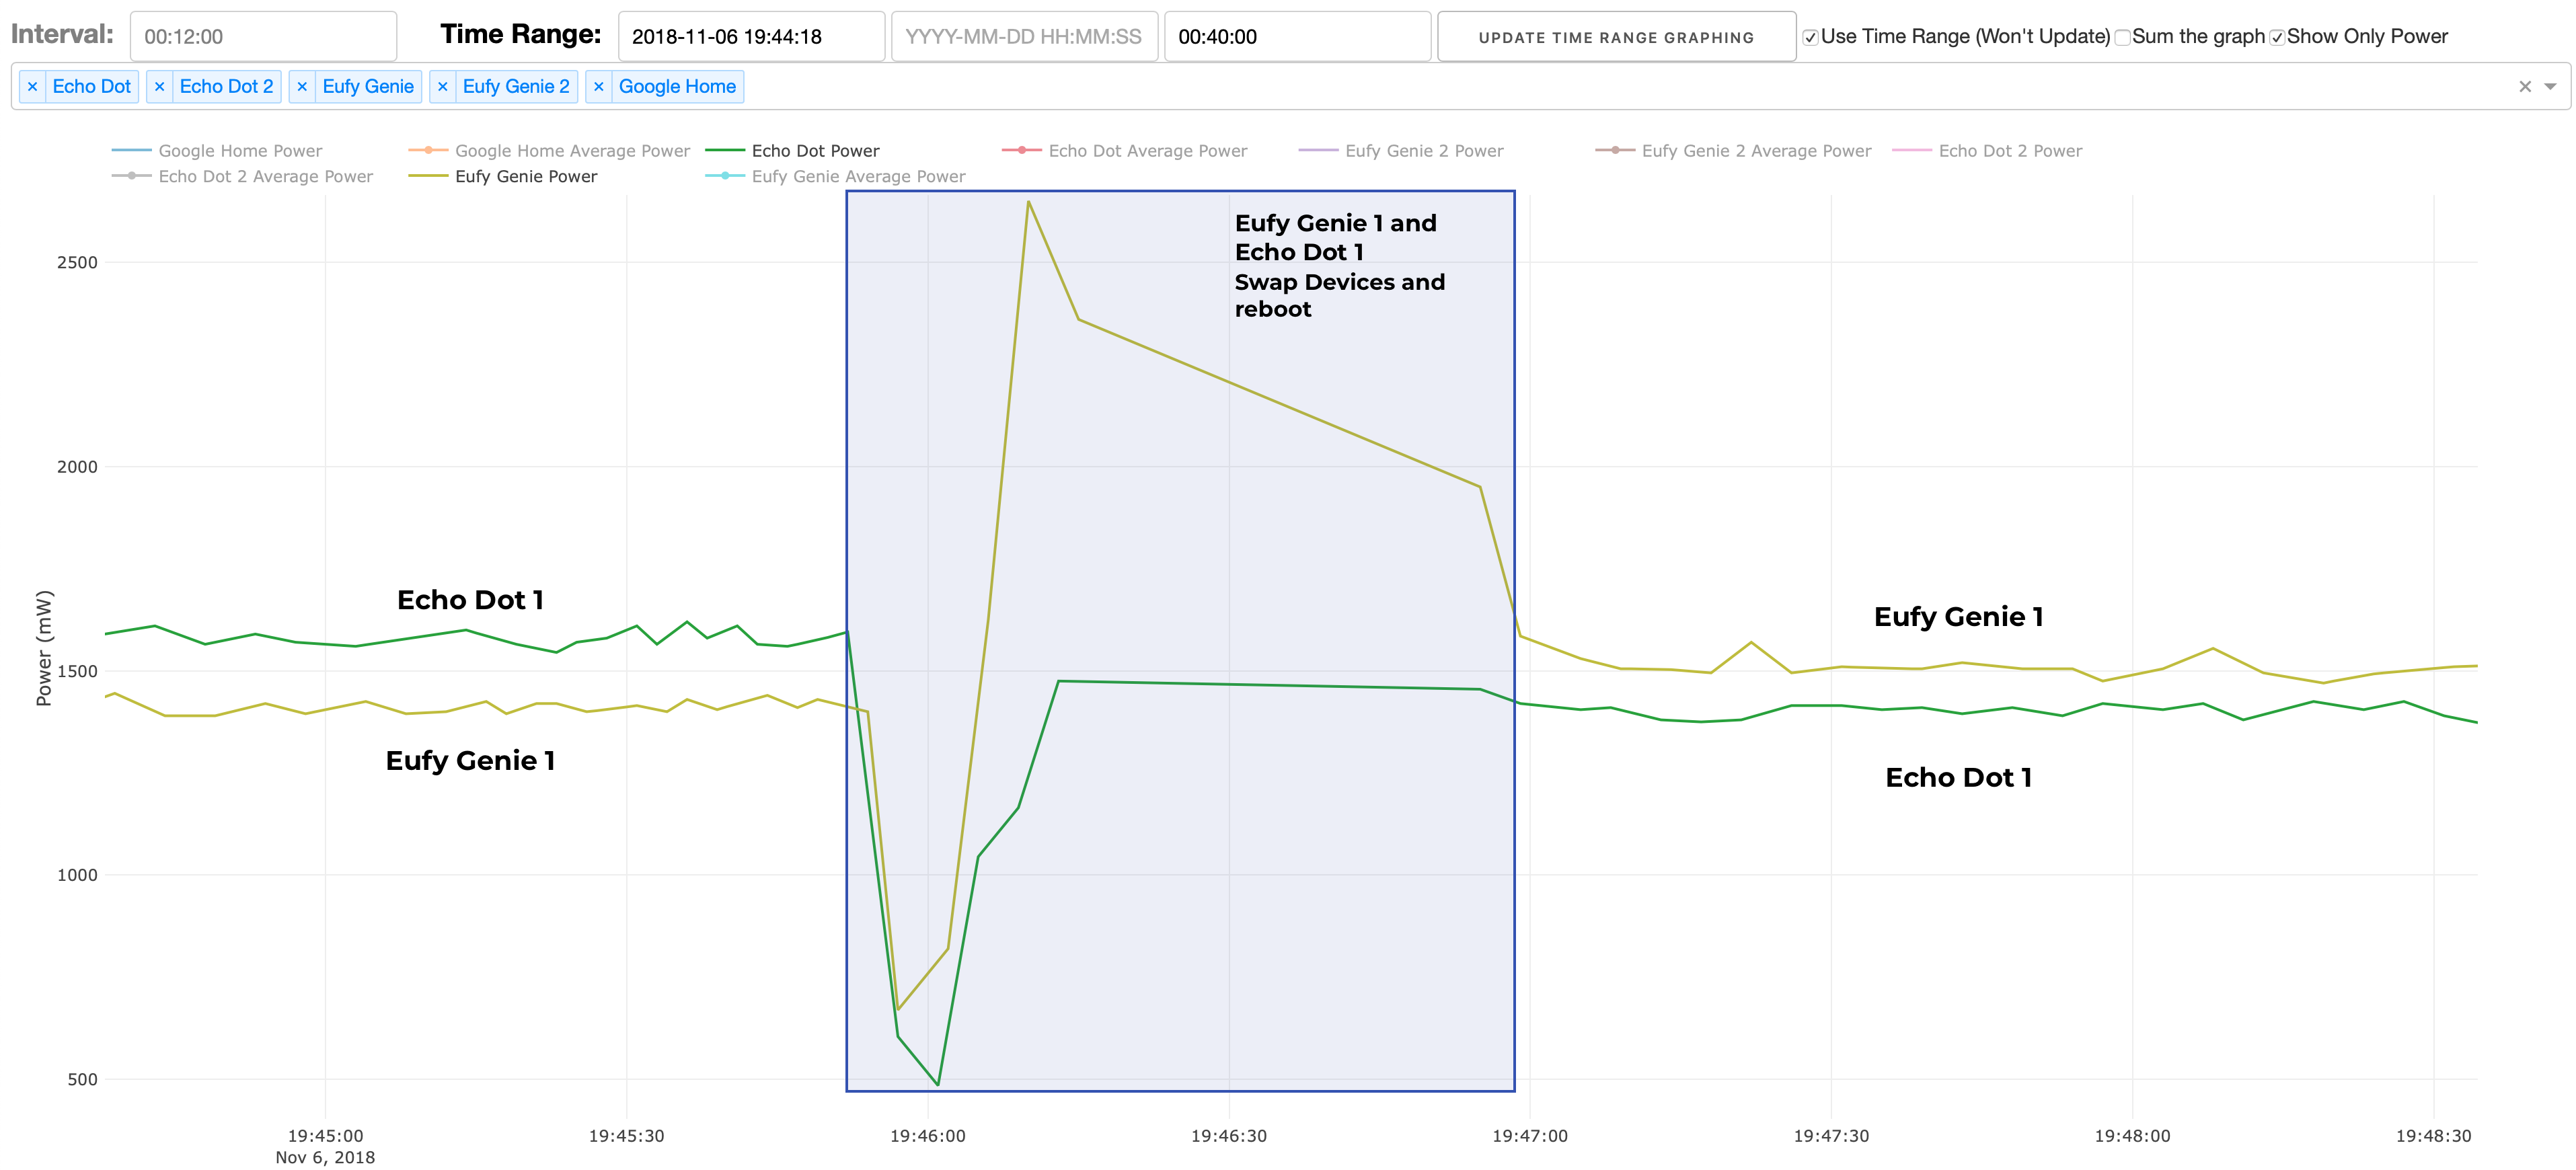
\includegraphics[width=1\textwidth]{figures/swapEufy1Echo1.png}
    \caption{Connected the Eufy Genie 1 to WeMo for `Echo Dot 1' and vice versa. The traces swap before and after switching.}
    \label{fig:swapEufy1Echo1}
\end{figure}

\begin{figure}[H]
    \centering
    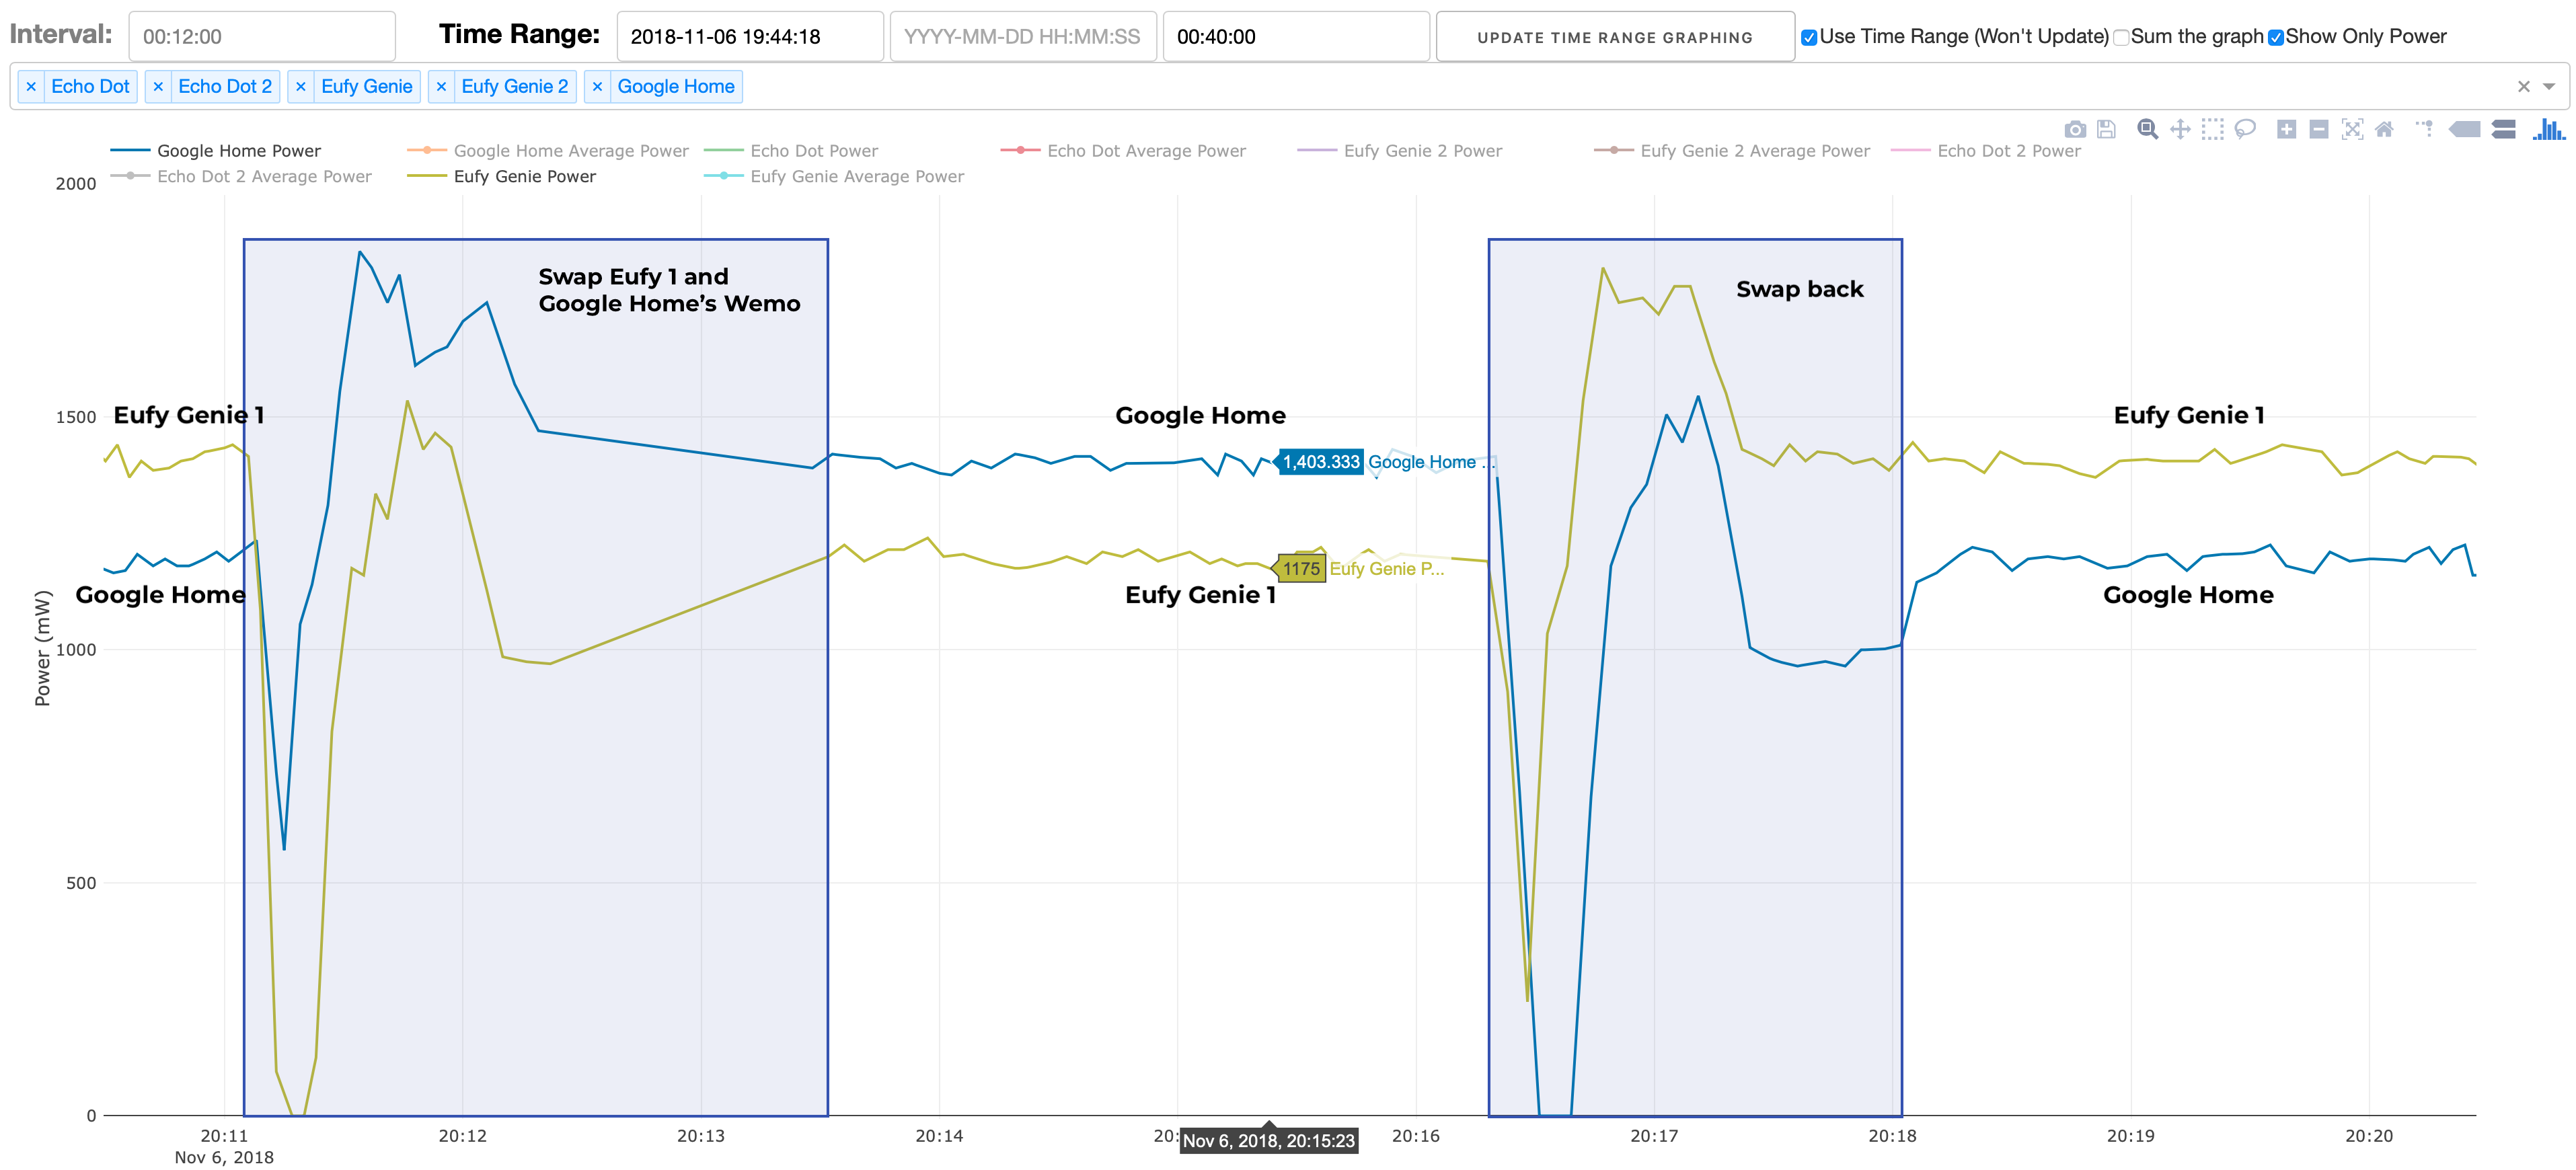
\includegraphics[width=1\textwidth]{figures/swapEufy1Home.png}
    \caption{Connected the Google Home to WeMo for `Eufy Genie 1' and vice versa. The traces swap before and after switching.}
    \label{fig:swapEufy1Home}
\end{figure}

\section{Whole Database}
\label{wholeDB}
When examining the whole database, most of the traffic is TCP packets. The second most significant protocol is UDP. The amount of packets using each protocol are shown in \ref{fig:tcpudp}. This figure is an example of some information that can be acquired from the database.

It shows the percentage of certain protocols that would pass through a typical home, adding to the fingerprint of IoT devices. Refer to Frawley's paper for more information on trends in the whole database\ref{frawleyPaper}.

\label{Whole Database}
\begin{figure}[H]
  \centering
    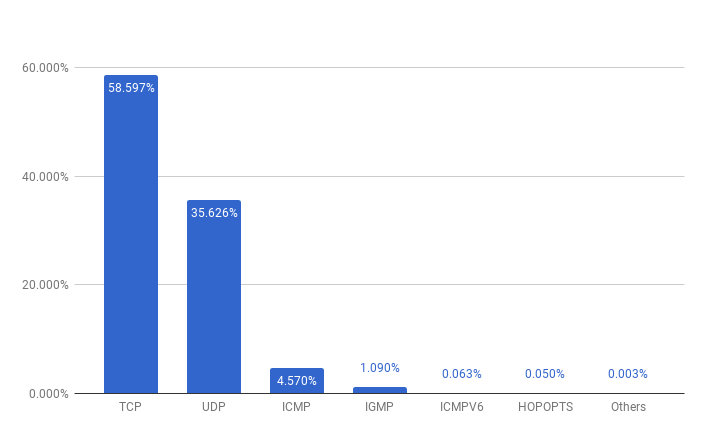
\includegraphics[width=1\textwidth]{tcpudp}
  \caption{Internet and Transport Layer Protocols in Database}
  \label{fig:tcpudp}
\end{figure}

\section{General Analysis}
\label{General Analysis}
The figures shown in this section give examples on how the database and grapher tool can be used. The figures also demonstrate a strong correlation between what the device is doing and its network/power usage, serving as data to fingerprint each smart speaker.

Frawley's paper contains a more in-depth analysis on this section and includes GeoIP \cite{maxmind} information from Cal Poly's ITS servers \cite{its} that highlights the locations and companies the network packets are being sent to and recieved from. Frawley's paper also includes data of unencrypted packets being sent and recieved along with the text within them. The rest of the sections include

\subsection{Smart Speakers}
\label{smartSpeakerResults}
This subsection covers the smart speakers' power and network usage in different scenarios.

\subsubsection{Google Home Mini}
The Google Home Mini's idle traffic broadcasts SSDP (Simple Service Discovery Protocol) packets once every minute. The SSDP packets are a discovery request packet for every IoT device on the network that supports UPnP (Universal Plug and Play). At which point devices such as the Echo Dot, Samsung TV, streaming devices, and the Chromebook respond with information about themselves in a .xml file. This XML file contains details regarding the device operating system and more. Google also sends encrypted TCP packets to Google every 10 minutes. The Google Home Mini's idle traffic is shown in figure \ref{fig:home}. The high peaks are the encrypted TCP packets, and the smaller spikes are the SSDP/UPnP packets.

\begin{figure}[H]
  \centering
    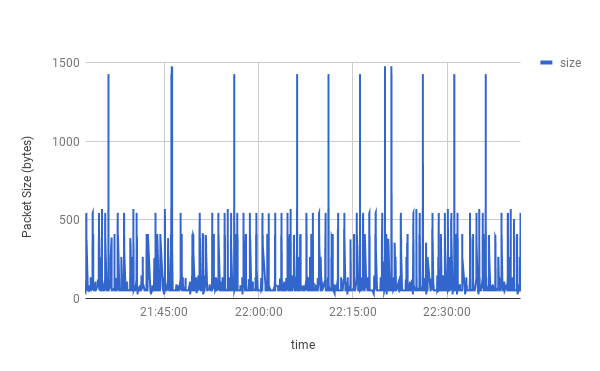
\includegraphics[width=0.9\textwidth]{home1hr}
  \caption{Idle Traffic of Google Home Over 1 Hour Period}
  \label{fig:home}
\end{figure}

A graph of the Google Home Mini's network and power usage under various commands are shown in the figure \ref{fig:homequery}. The Google Home Mini is first asked for the news and then told to stop. After waiting for 40 minutes, we ask it for the weather forecast.

\begin{figure}[H]
  \centering
    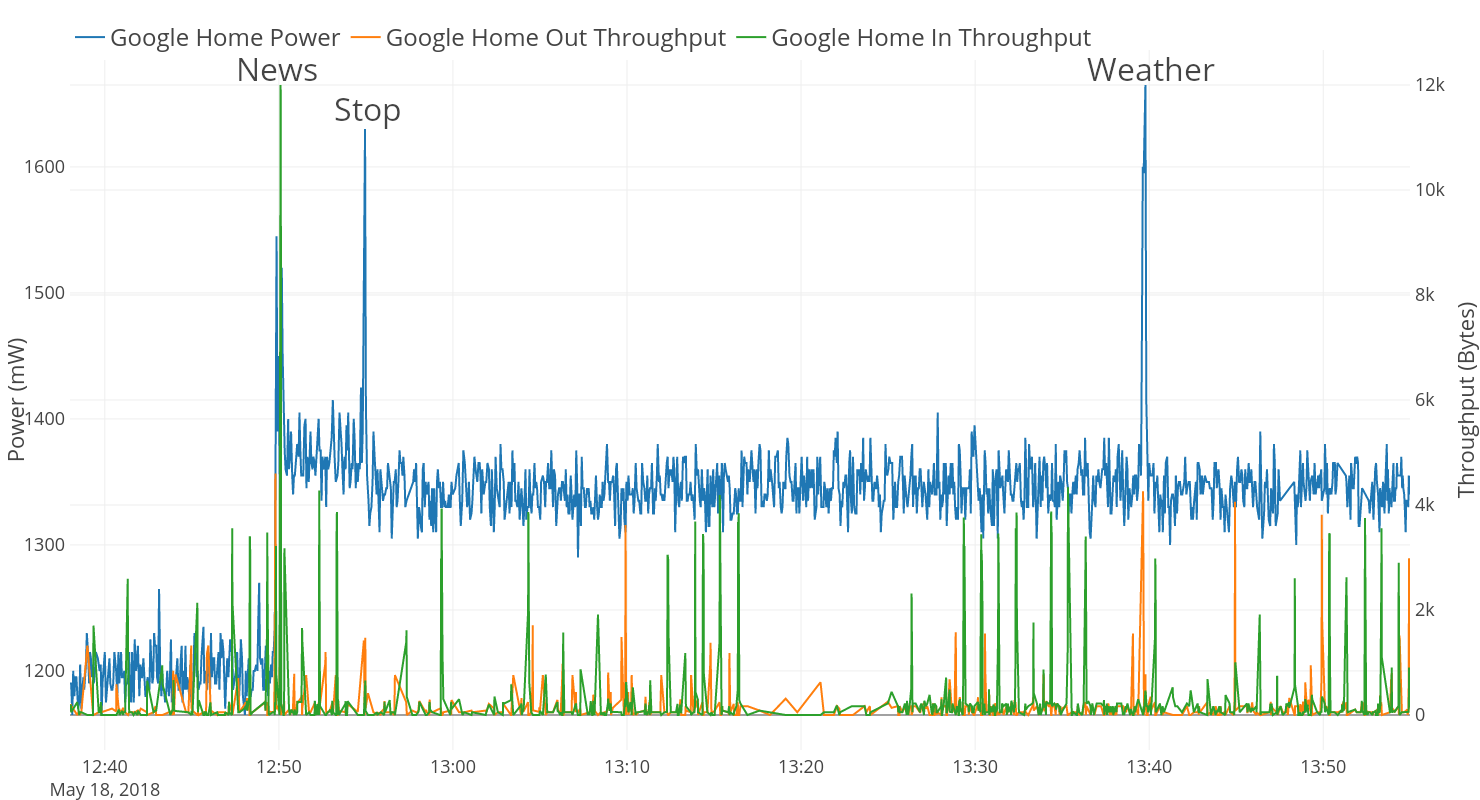
\includegraphics[width=1\textwidth]{homequery}
  \caption{Home Mini Response to News and Weather}
  \label{fig:homequery}
\end{figure}

\subsection{Streaming Devices}
\label{Streaming Devices}
This subsection covers the streaming devices' power and network usage in different scenarios.

\subsubsection{Google Chrome Cast}
\begin{figure}[H]
  \centering
  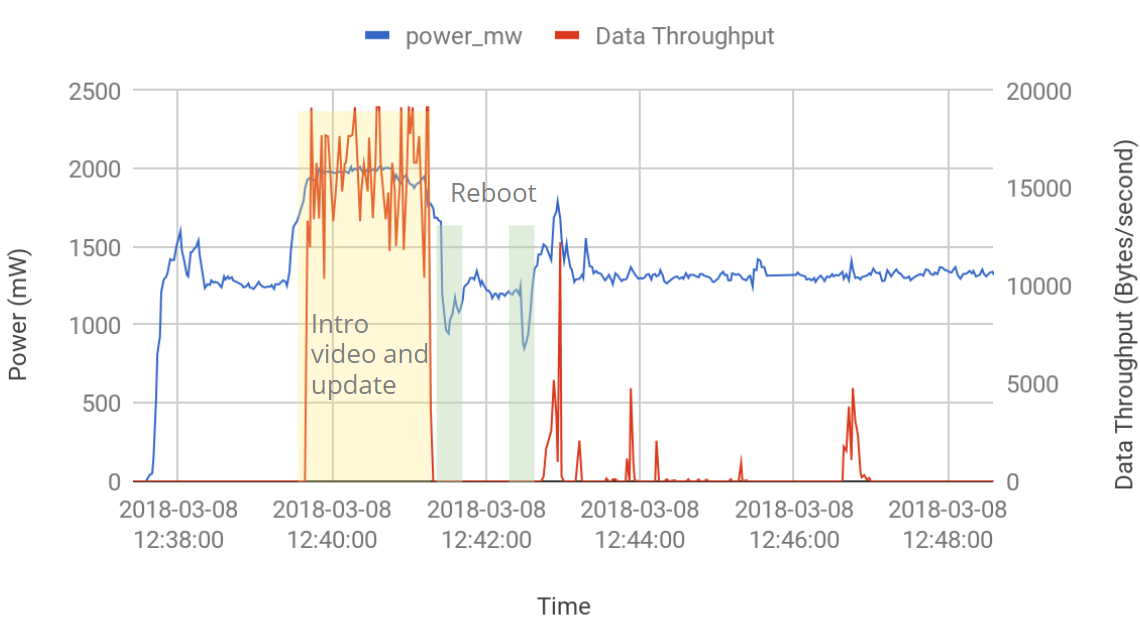
\includegraphics[width=1\textwidth]{ccboth}
  \caption{Chromecast First Time Boot Network Traffic and Power Consumption}
  \label{fig:ccboth}
\end{figure}

The Chrome Cast startup graph is shown in figure \ref{fig:ccboth}. On startup, the Chrome Cast shows an intro tutorial video and downloads a firmware update. After rebooting twice, it is ready to go.

\begin{figure}[H]
  \centering
  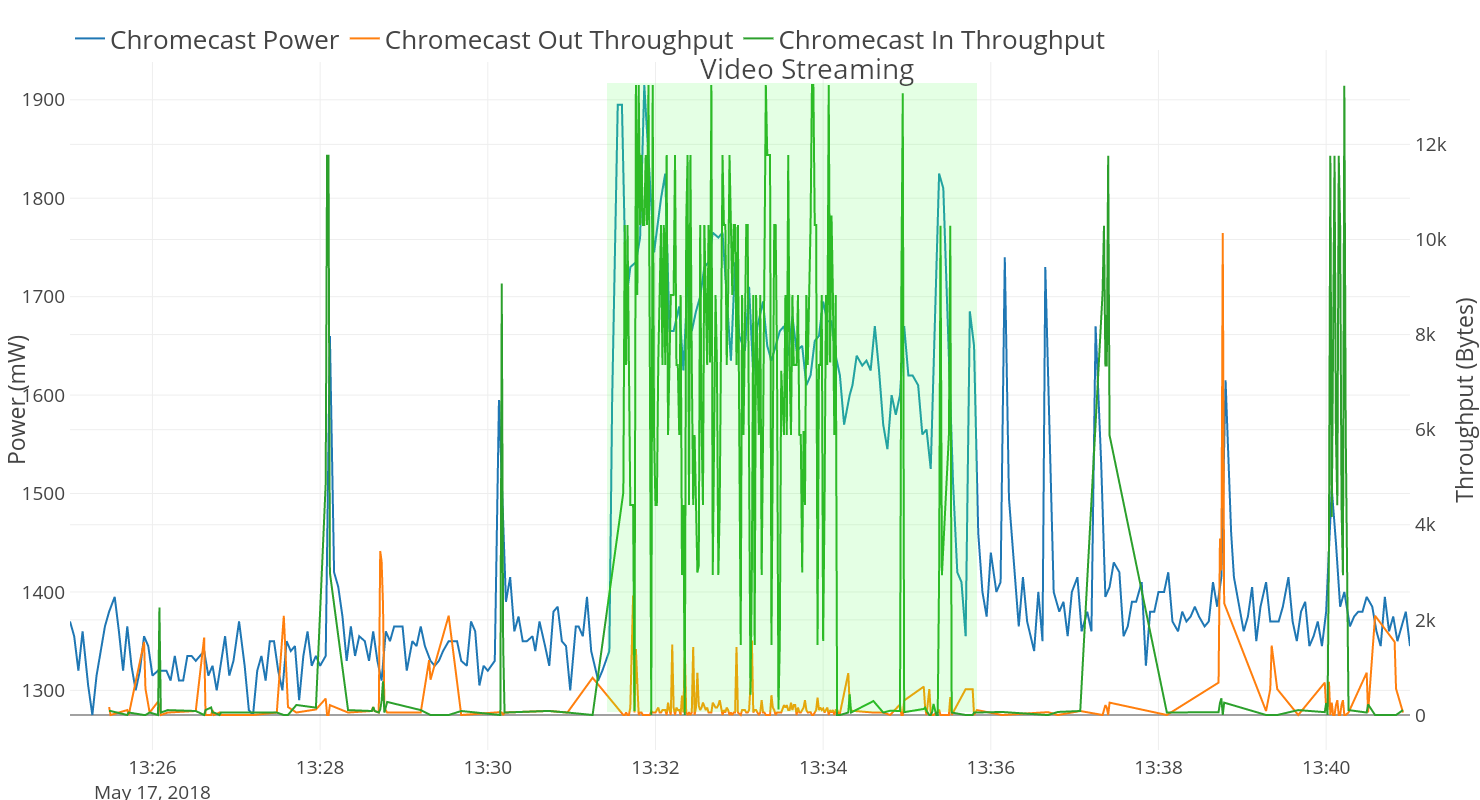
\includegraphics[width=1\textwidth]{ccstreaming}
  \caption{Chromecast Video Streaming}
  \label{fig:ccstream}
\end{figure}

The Chrome Cast streaming graph is shown in figure \ref{fig:ccstream}. In this time frame, the chrome cast streams video in the marked box.

\begin{figure}[H]
  \centering
  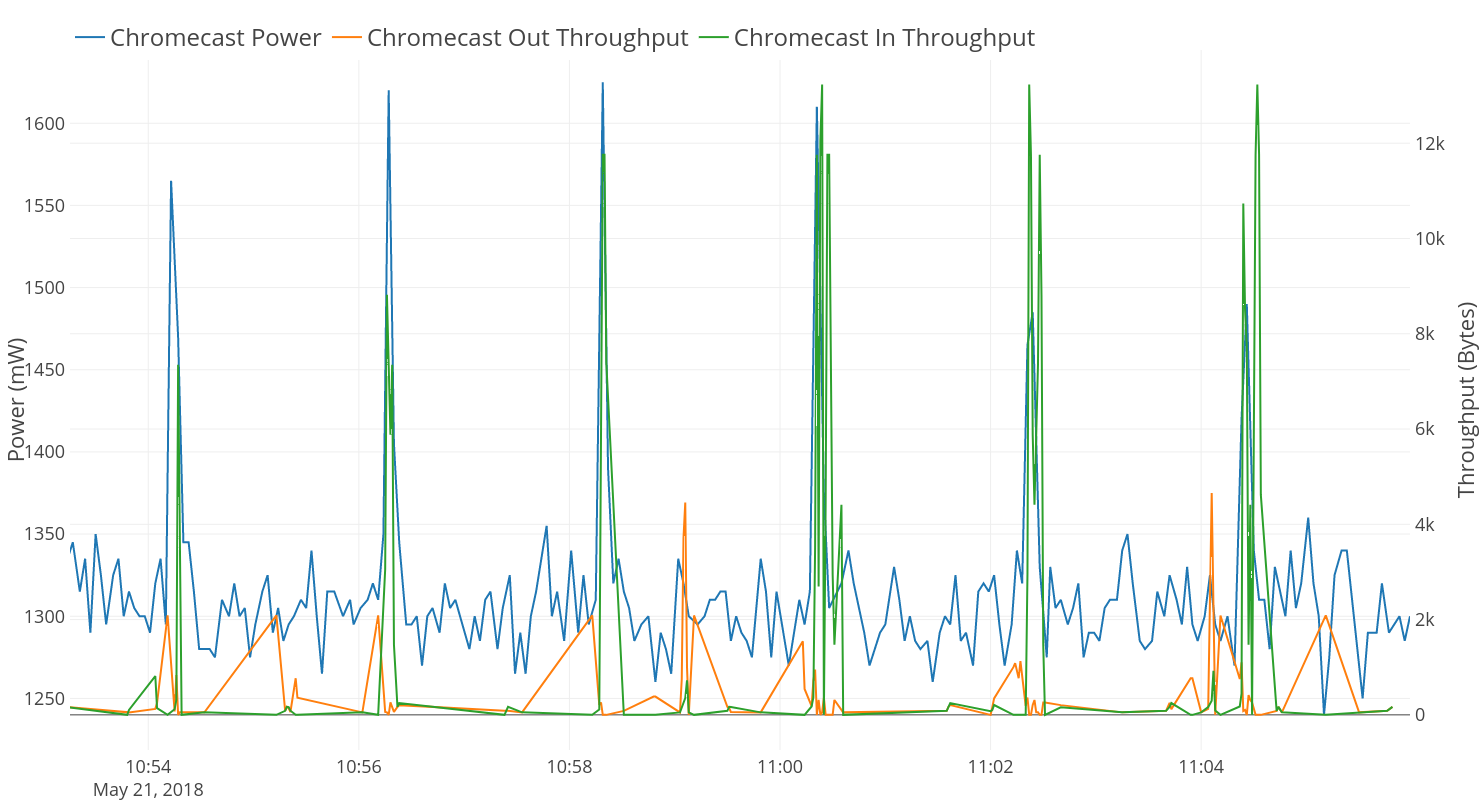
\includegraphics[width=1\textwidth]{chromecastbg}
  \caption{Chromecast Idle Traffic}
  \label{fig:ccbg}
\end{figure}

Additionally, the Chrome Cast idle graph is shown in figure \ref{fig:ccbg}. In this time frame, there are consistent spikes to the chrome cast every 2 minutes. During these spikes, the chrome cast is showing a new background that it downloads from Google Servers.

\subsubsection{Amazon Fire Stick}

\begin{figure}[H]
  \centering
  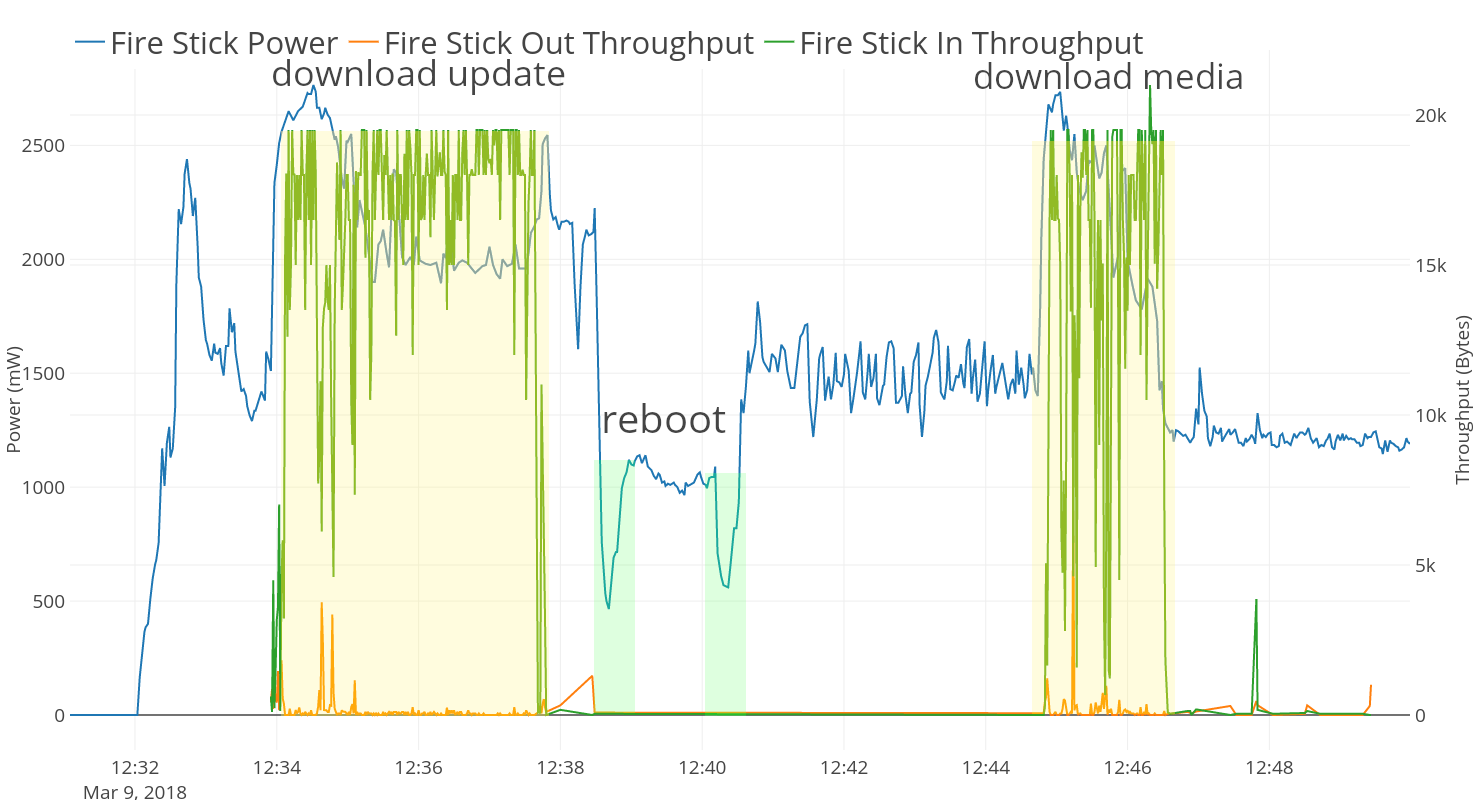
\includegraphics[width=1\textwidth]{fireboot}
  \caption{Fire TV Stick First Time Boot Network Traffic and Power Consumption}
  \label{fig:fireboth}
\end{figure}

The Amazon Fire Stick startup graph is shown in figure \ref{fig:fireboth}. On first boot, the fire stick downloads an update, reboots twice, then downloads certificates from Symantec and Verisign.

When streaming, the Fire Stick increases throughput and power usage with a spike at the beginning and end of streaming in power usage as shown in figure \ref{fig:fsyt}.

\begin{figure}[H]
  \centering
  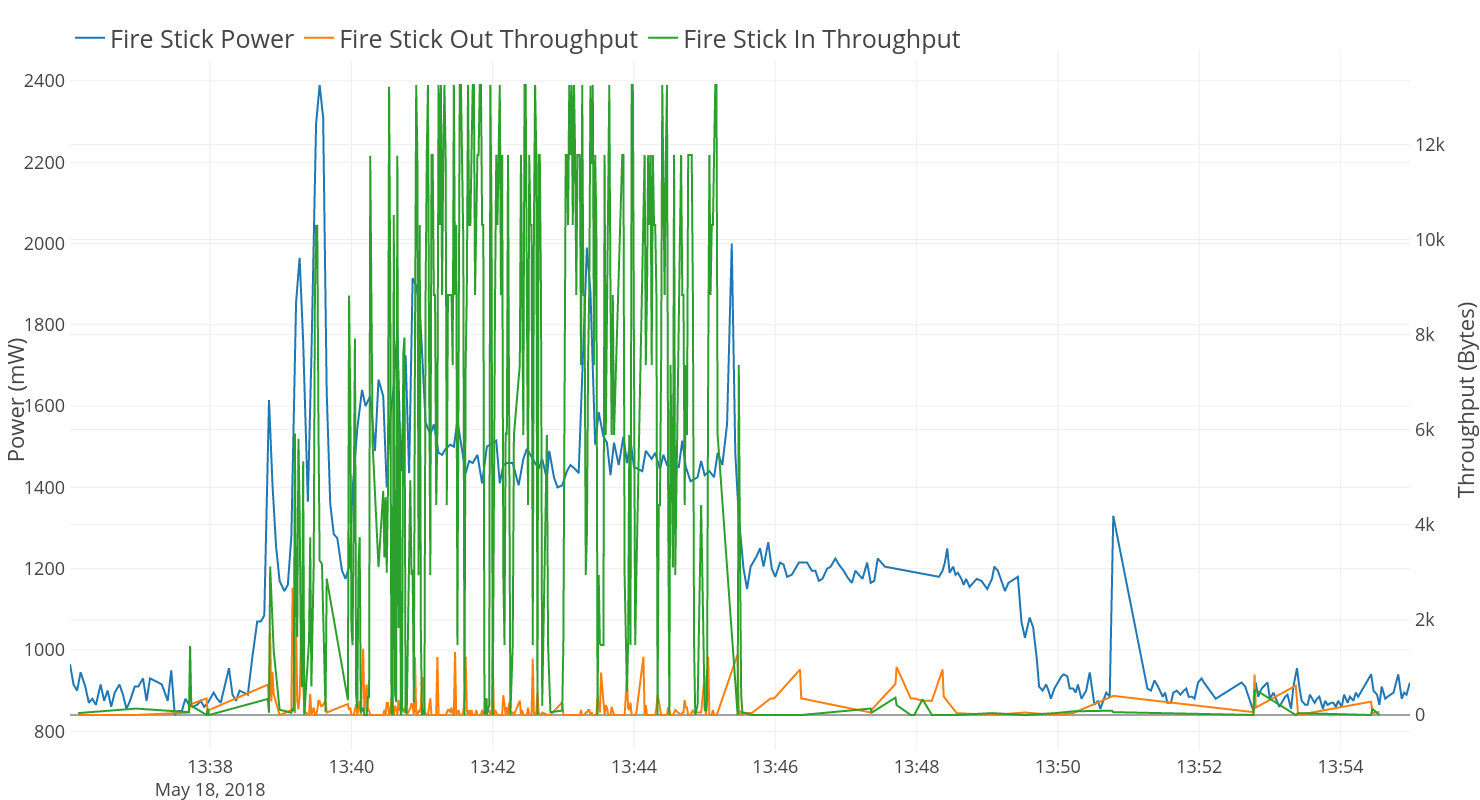
\includegraphics[width=1\textwidth]{fsyt}
  \caption{Fire TV Stick Video Streaming}
  \label{fig:fsyt}
\end{figure}

\subsubsection{Roku Express}
When streaming, the Roku's power usage and network throughput rise and stay at a constant level until the video streaming is complete. At which point it drops back down when done.

\begin{figure}[H]
  \centering
  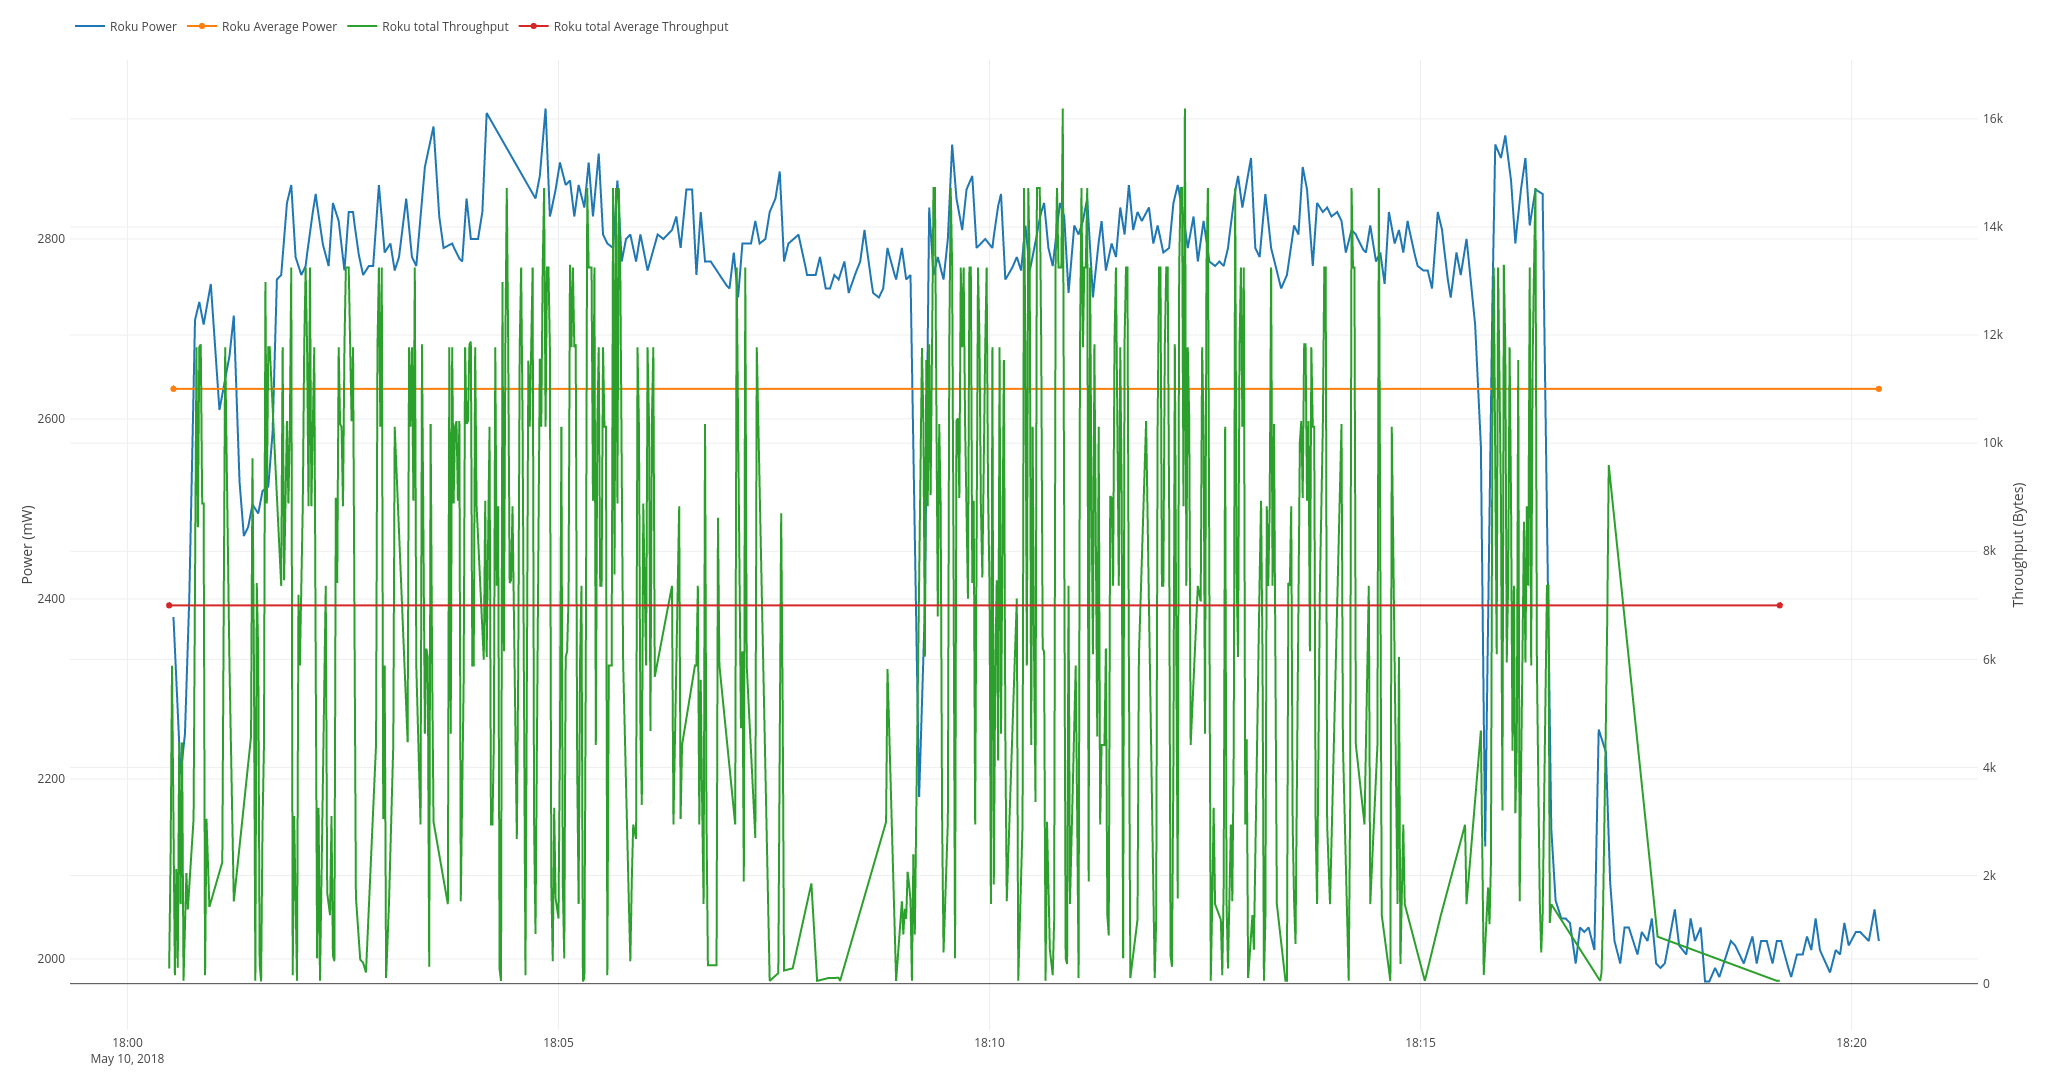
\includegraphics[width=1\textwidth]{figures/rokuStreaming.png}
  \caption{Roku Express Video Streaming}
  \label{fig:rokuStreaming}
\end{figure}

\subsection{General Analysis Discussion}
From all the figures in this section, there is a visual correlation between network/power usage and what the devices is doing. During periodic updates the smart speakers and streamign devices would have periodic network/power usage spikes. While streaming, the power/network usage would increase for the period of the stream. This strong correlation was the first steps in using the database and visualizer tool for visual pattern recognition, proving its viability.

\section{Power Analysis on Smart Speakers}
\label{Power Analysis on Smart Speakers}

After determining a strong correlation between network/power usage to device operation, this section begins to focus on power usage over time. Significant analysis on network usage had already been done as shown in the previous works \ref{Previous Work} section. This section highlights initial power findings which shows that a lot can be determined from visually examing a power graph over time in subsection \ref{Echo Dot Brightness Sensor}. Once discovering the insight a power trace can provide, the research focused on overarching goal to see if given a graph of a house's total power usage, is it possible to determine the device in use. This paper will focus on smart speakers' power usage to test this hypotheses.

But before doing that, this section examines the power usage of the smart speakers seperately before examining total power usage in section \ref{sumPowerGraph}. Subsection \ref{Baseline Speaker Power} examines idle power of smart speakers seperately, showing that a smart speaker can be determined from its idle power (to a small extent). Then subsection \ref{Smart Speaker Power Spikes When Asked for Weather} shows that through visual examination of a power trace of an individual smart speaker, we can tell what smart speaker is in use.

\subsection{Echo Dot Brightness Sensor}
\label{Echo Dot Brightness Sensor}
One interesting finding from the Echo Dot is that it has a light monitor. When turning on the lights, the LEDs on the Echo Dot brighten to adapt. The brightness change causes the Echo Dot to use more idle power as shown in figure \ref{fig:echolights}.

Figure \ref{fig:echolights} shows that the power usage of an Echo Dot can show if the lights are on in a house. This can help someone determine if someone is in their house or not or event what room they are in, introducing some privacy concerns.

\begin{figure}[H]
    \centering
    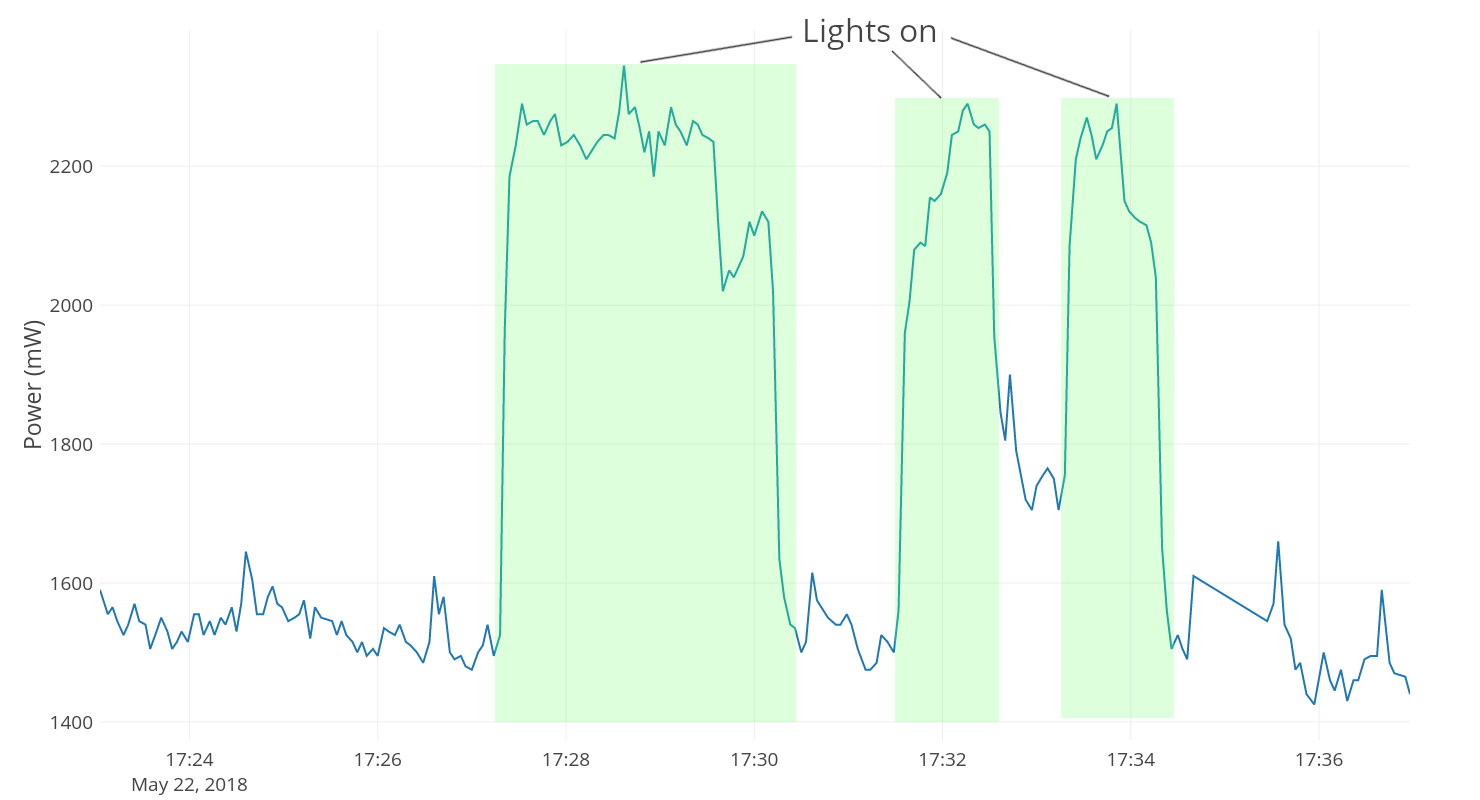
\includegraphics[width=1\textwidth]{echolights}
    \caption{Echo Dot Response to Lights}
    \label{fig:echolights}
\end{figure}

\subsection{Baseline Speaker Power}
\label{Baseline Speaker Power}
Once discovering how much a smart speaker's power usage can show, this section examines the power usage of each smart speaker while idle. Figure \ref{fig:baselineSpeakerPower} shows this from 1:00 AM to 2:30 AM when none of the devices are in use.

The Echo Dot 1 has the highest idle traffic as shown in the pink trace, the Echo Dot 2 has second highest idle traffic as shown in the green trace, the Eufy 1 and Eufy 2 have the same idle power usage as shown in the yellow and purple trace, then the Google Home has the lowest idle power usage as shown in the blue trace. With visual analysis, thesmart speaker can be matched to idle power usage. But the power usages can overlap between the Echo Dot 2 and Eufys. This would make it difficult to differentiate them and proves this method of device determination difficult. Also, when summing the power usages together, these idle traces would dissapear, with no way to differntiate what idle devices are contributing to the total power usage.

\begin{figure}[H]
    \centering
    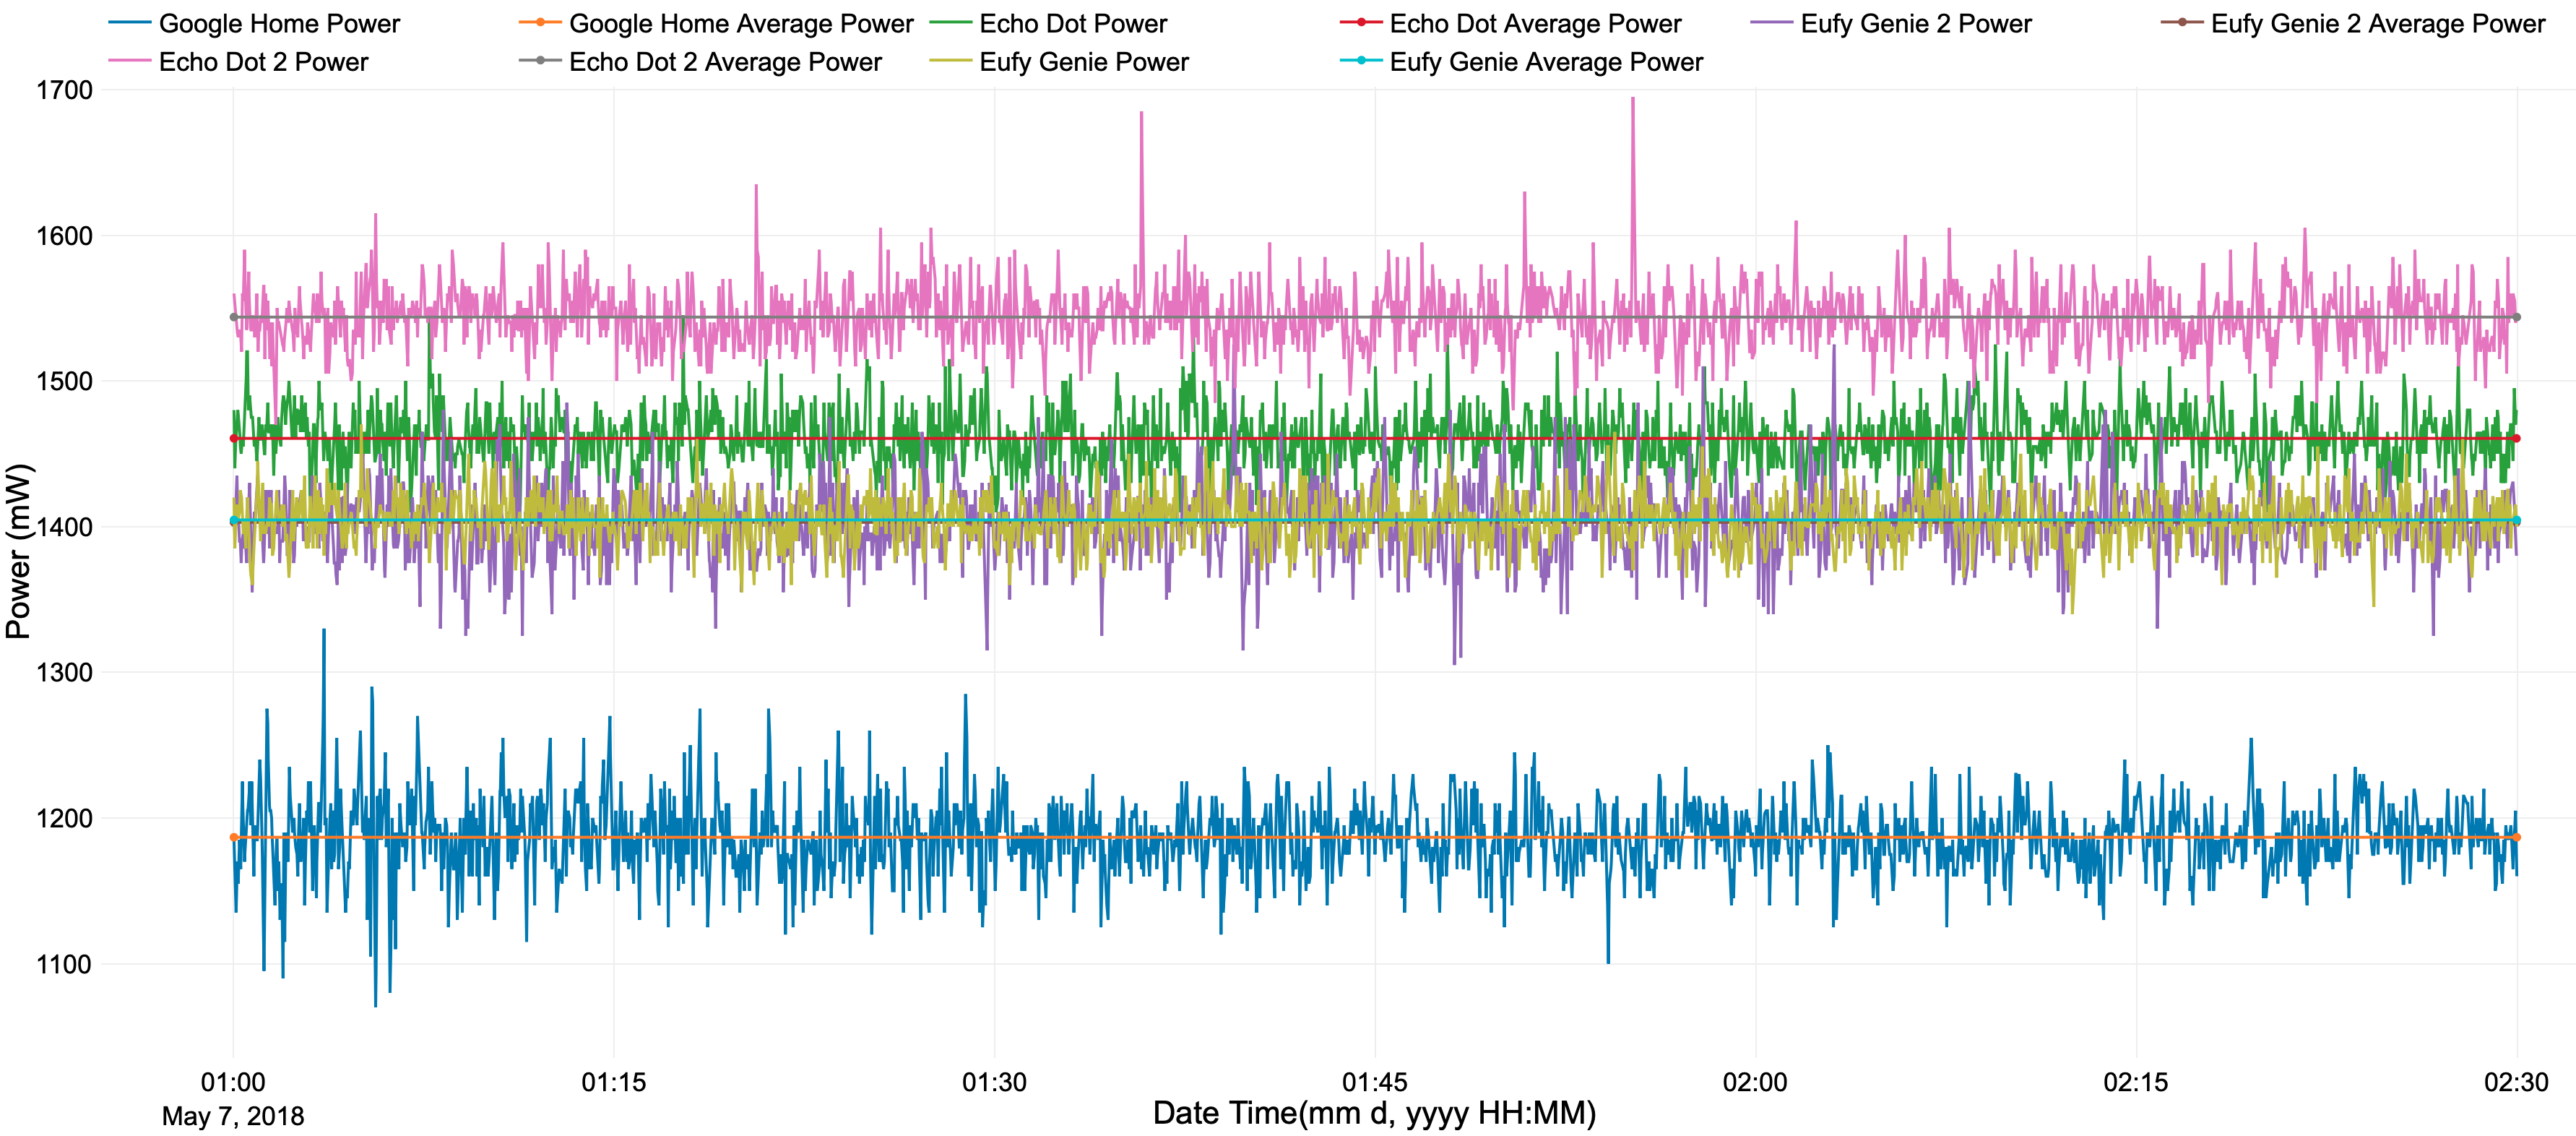
\includegraphics[width=1\textwidth]{baselineSpeakerPower.png}
    \caption{Baseline smart speaker power usage.}
    \label{fig:baselineSpeakerPower}
\end{figure}

\subsection{Smart Speaker Power Spikes When Asked for Weather}
\label{Smart Speaker Power Spikes When Asked for Weather}
This section continues to see if a smart speaker can be determined from an individual power trace, focusing on traces while the device is in use. This is shown in figure \ref{fig:speakerWeatherSeperate} where each device is asked for the weather 4 times.

In figure \ref{fig:speakerWeatherSeperate} there is a visual spike for each device while it is giving the weather forecast. Each device is highlighted while in use, showing 4 spikes. The Google Home was queried for the weather 5 times, thus containing an extra spike. From this, we can determine a Eufy trace if it has small 400 mW spikes, the Google Home if there are medium 600 mW spikes, and the Echo Dot if there are large 2,100 mW spikes. This implies that a device can be determined from a power trace if the device is asked for the weather. In the next section, more use cases are analyzed and the traces are summed together to more closely simulate a shared home powerline.

\begin{figure}[H]
    \centering
    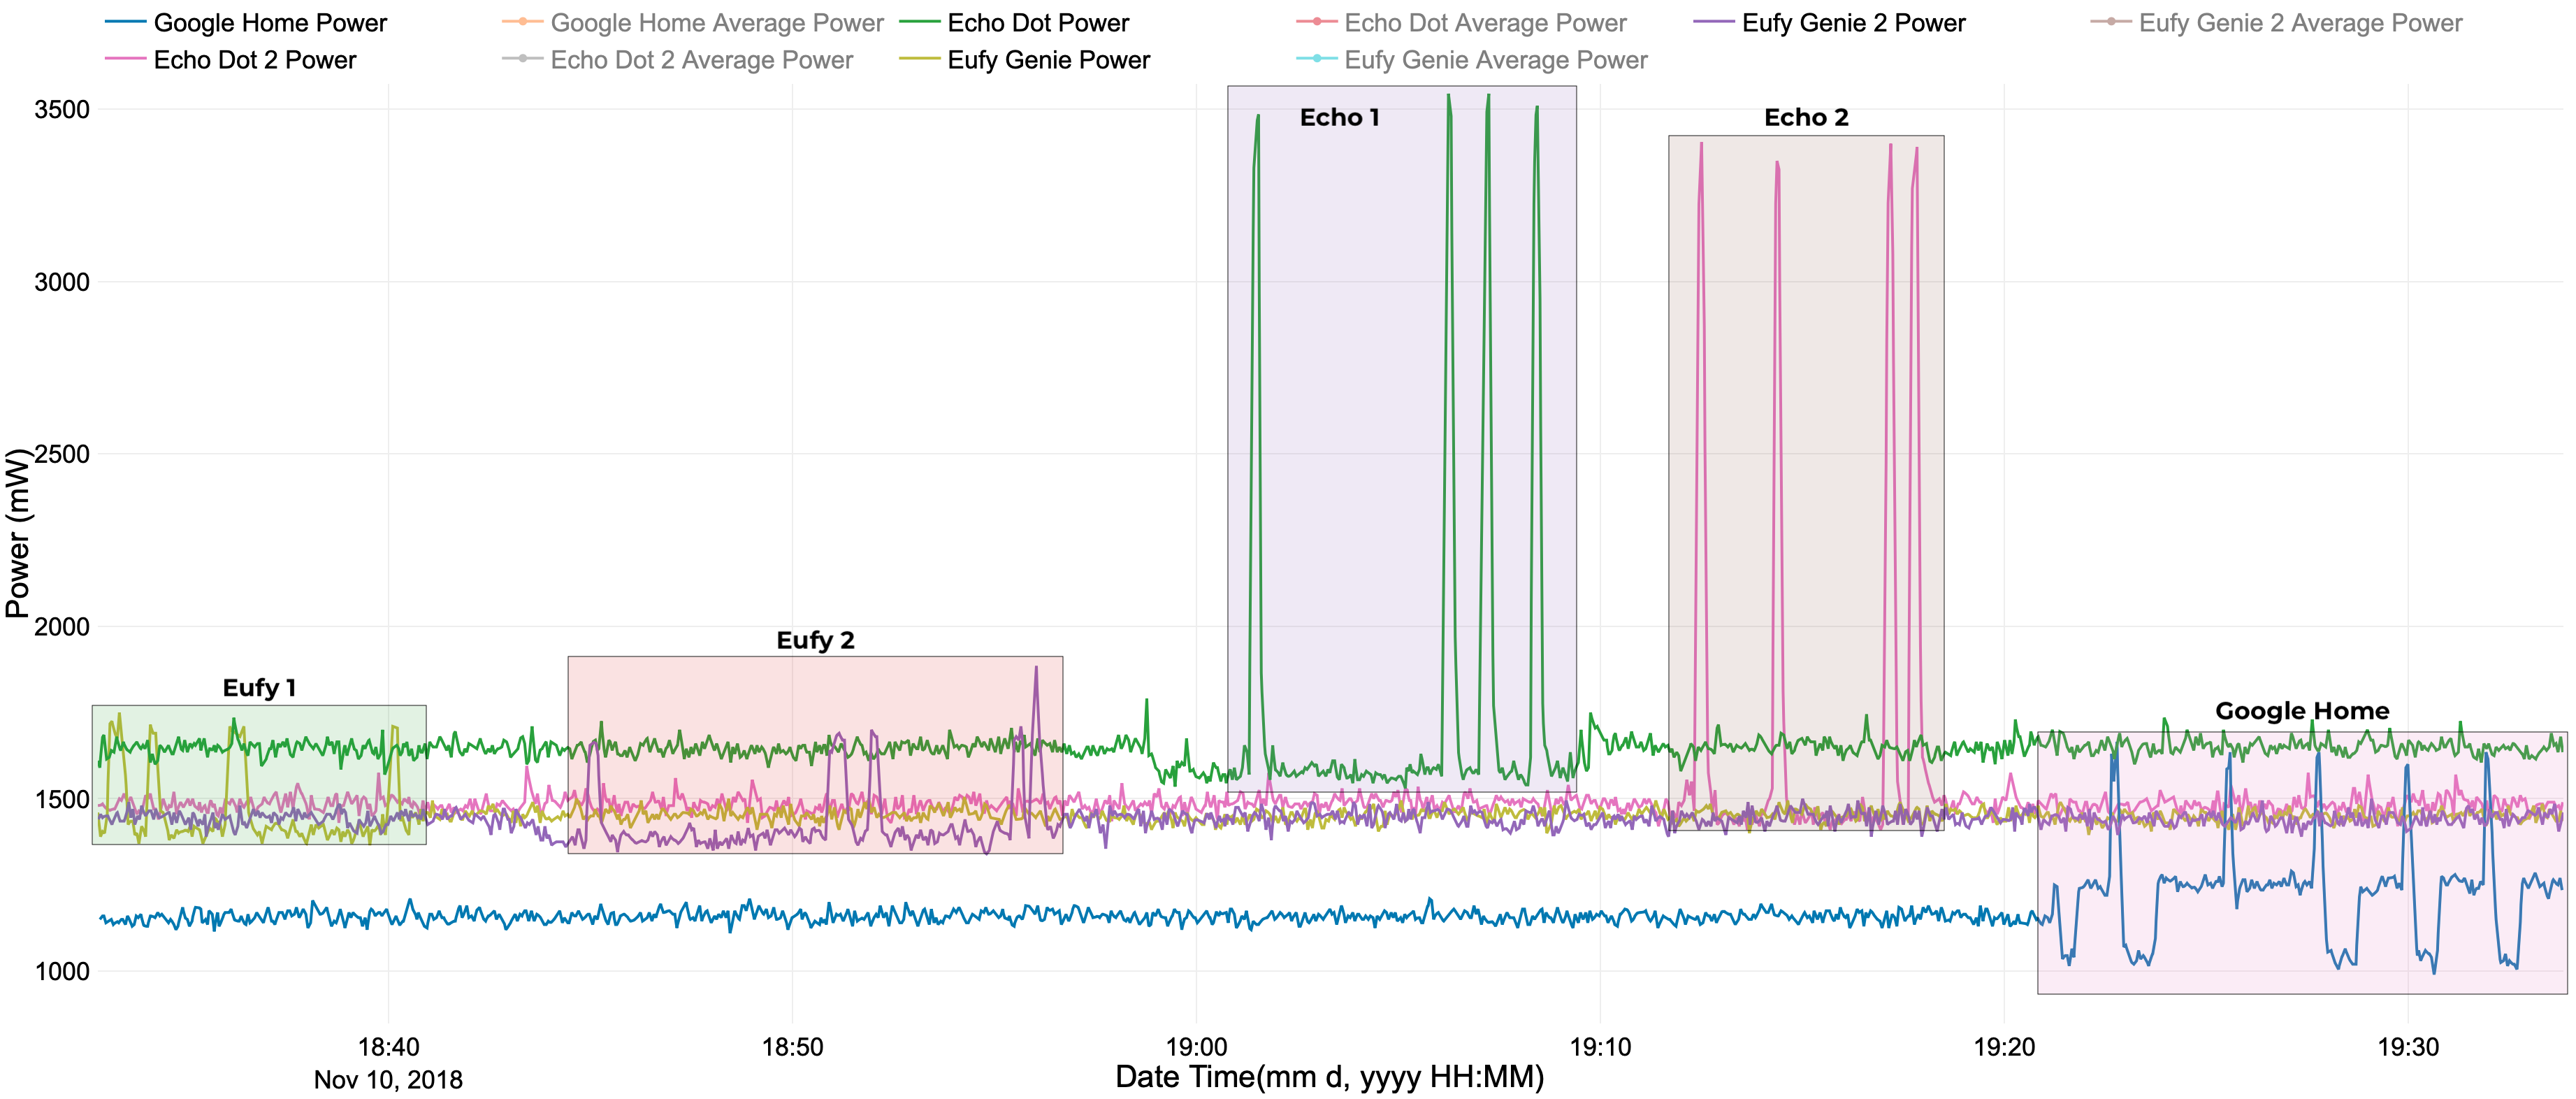
\includegraphics[width=1\textwidth]{speakerWeatherSeperate.png}
    \caption{Smart speakers' power usage when asked `what\'s the weather' four times.}
    \label{fig:speakerWeatherSeperate}
\end{figure}

\section{Summed Power Graph}
\label{sumPowerGraph}
This section visually analyzes the power usages of all 5 of the smart speakers summed together under different commands.

The first graph in figure \ref{fig:weatherSum} is shown in a time frame where each device was unmuted and muted for a period. This shows if muting and unmuting the devices affected the power or network usage. There are changes on the first runthrough, but when repeating the process nothing happens. Further runthroughs show that the power usage stayed the same. In the last half of the graph we queried each smart speaker for the weather while all other smart speakers were muted at the 18:30 mark. We query each device 3-4 times for the weather. The Eufy had the smallest spike for the ``what\'s the weather'' command at 400 mW, then the Google Home at 600 mW, and finally the Echo Dot at 2000 mW.

\begin{figure}[H]
  \centering
  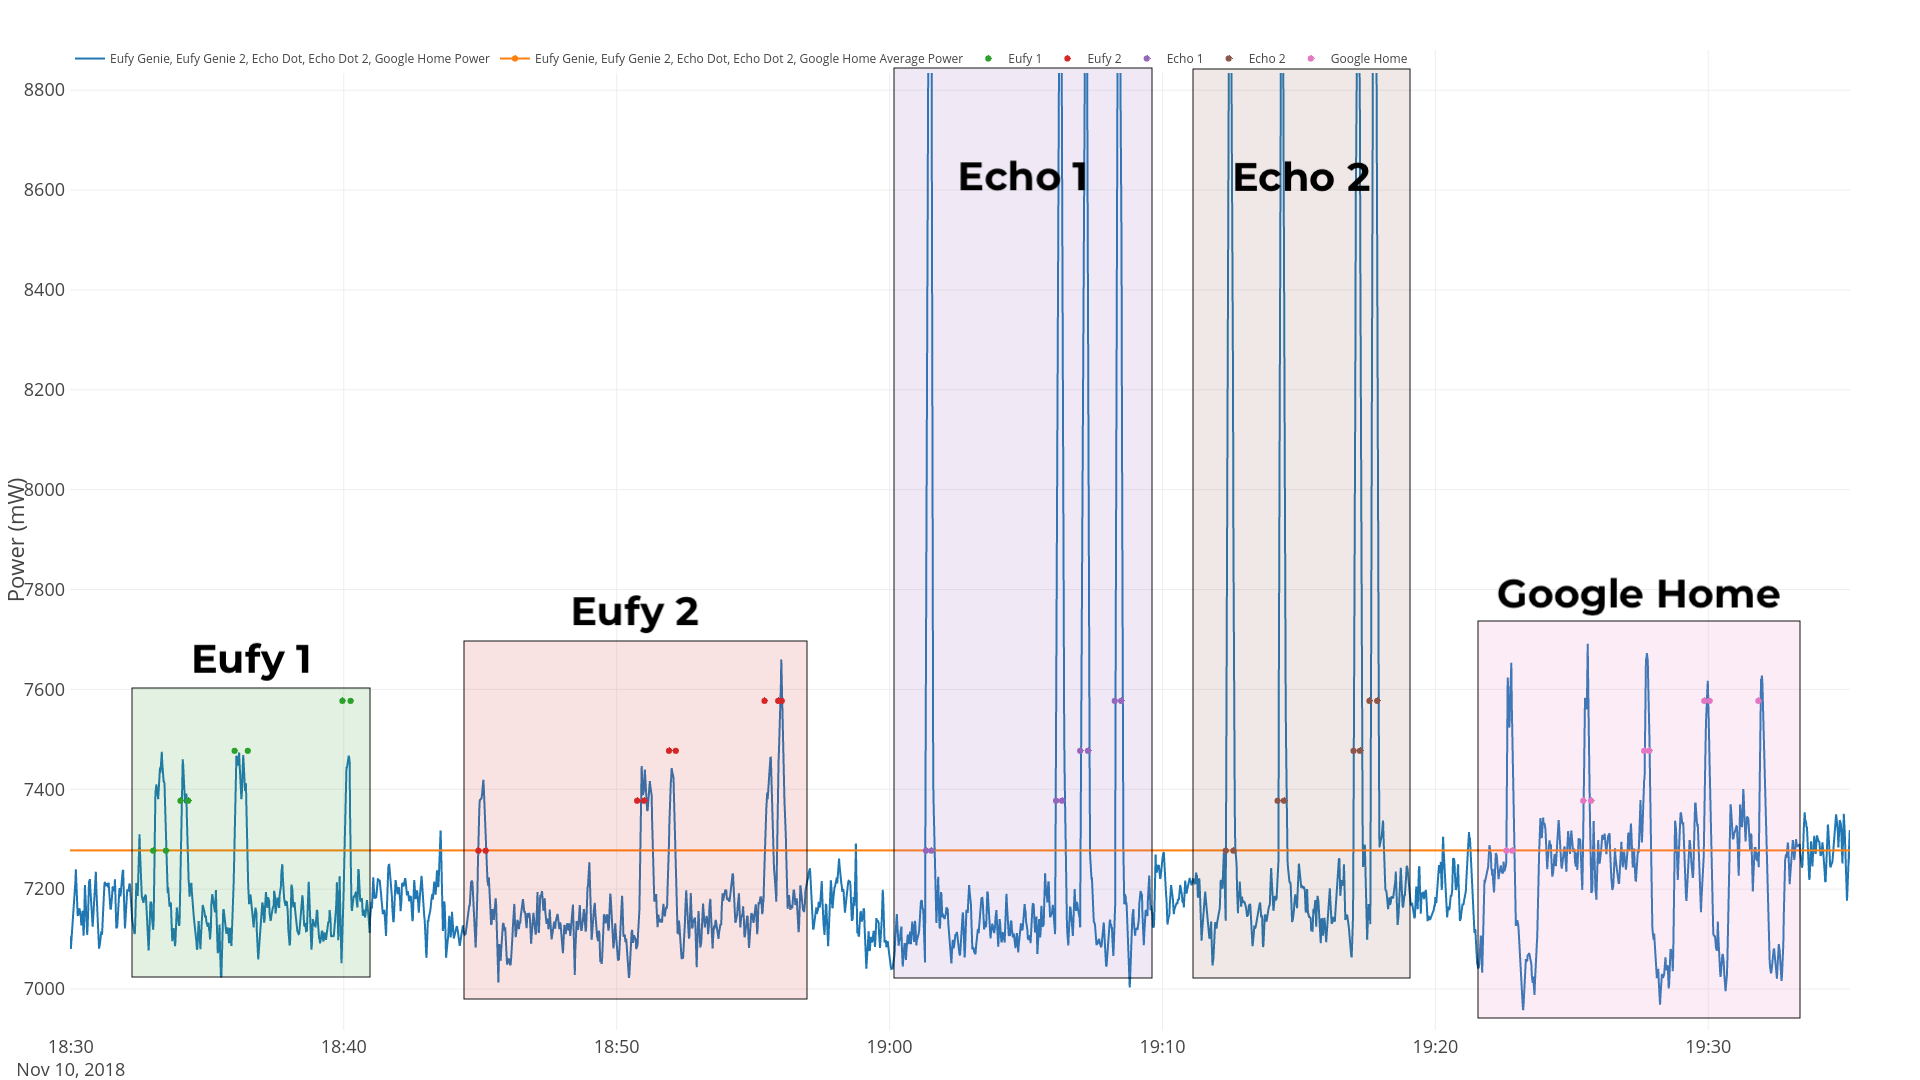
\includegraphics[width=1\textwidth]{figures/weatherSum.png}
  \caption{5 Smart Speakers Power Summed Up. Toggled the mute button and queried each device for the weather.}
  \label{fig:weatherSum}
\end{figure}

The next graph, \ref{fig:mixedNewsSum}, shows the smart speakers power usage when asked for the news. Each speaker was asked for the news. This graph and the rest of the summed graphs in this section use the same notation for signifying commands. Two corresponding dots of the same color signify the start and end of the command for a specific device. If the dots are on another level, then this command has been repeated another time.

In figure \ref{fig:mixedNewsSum}, all devices have a spike at the beginning and end of the command and maintain a steady energy usage in between that is slightly higher than the idle energy used. The peak to peak spike of the Eufy Genie is the smallest at 350 mW, then the Google Home at 500 mW, and finally the Echo Dot at 1900 mW.

\begin{figure}[H]
  \centering
  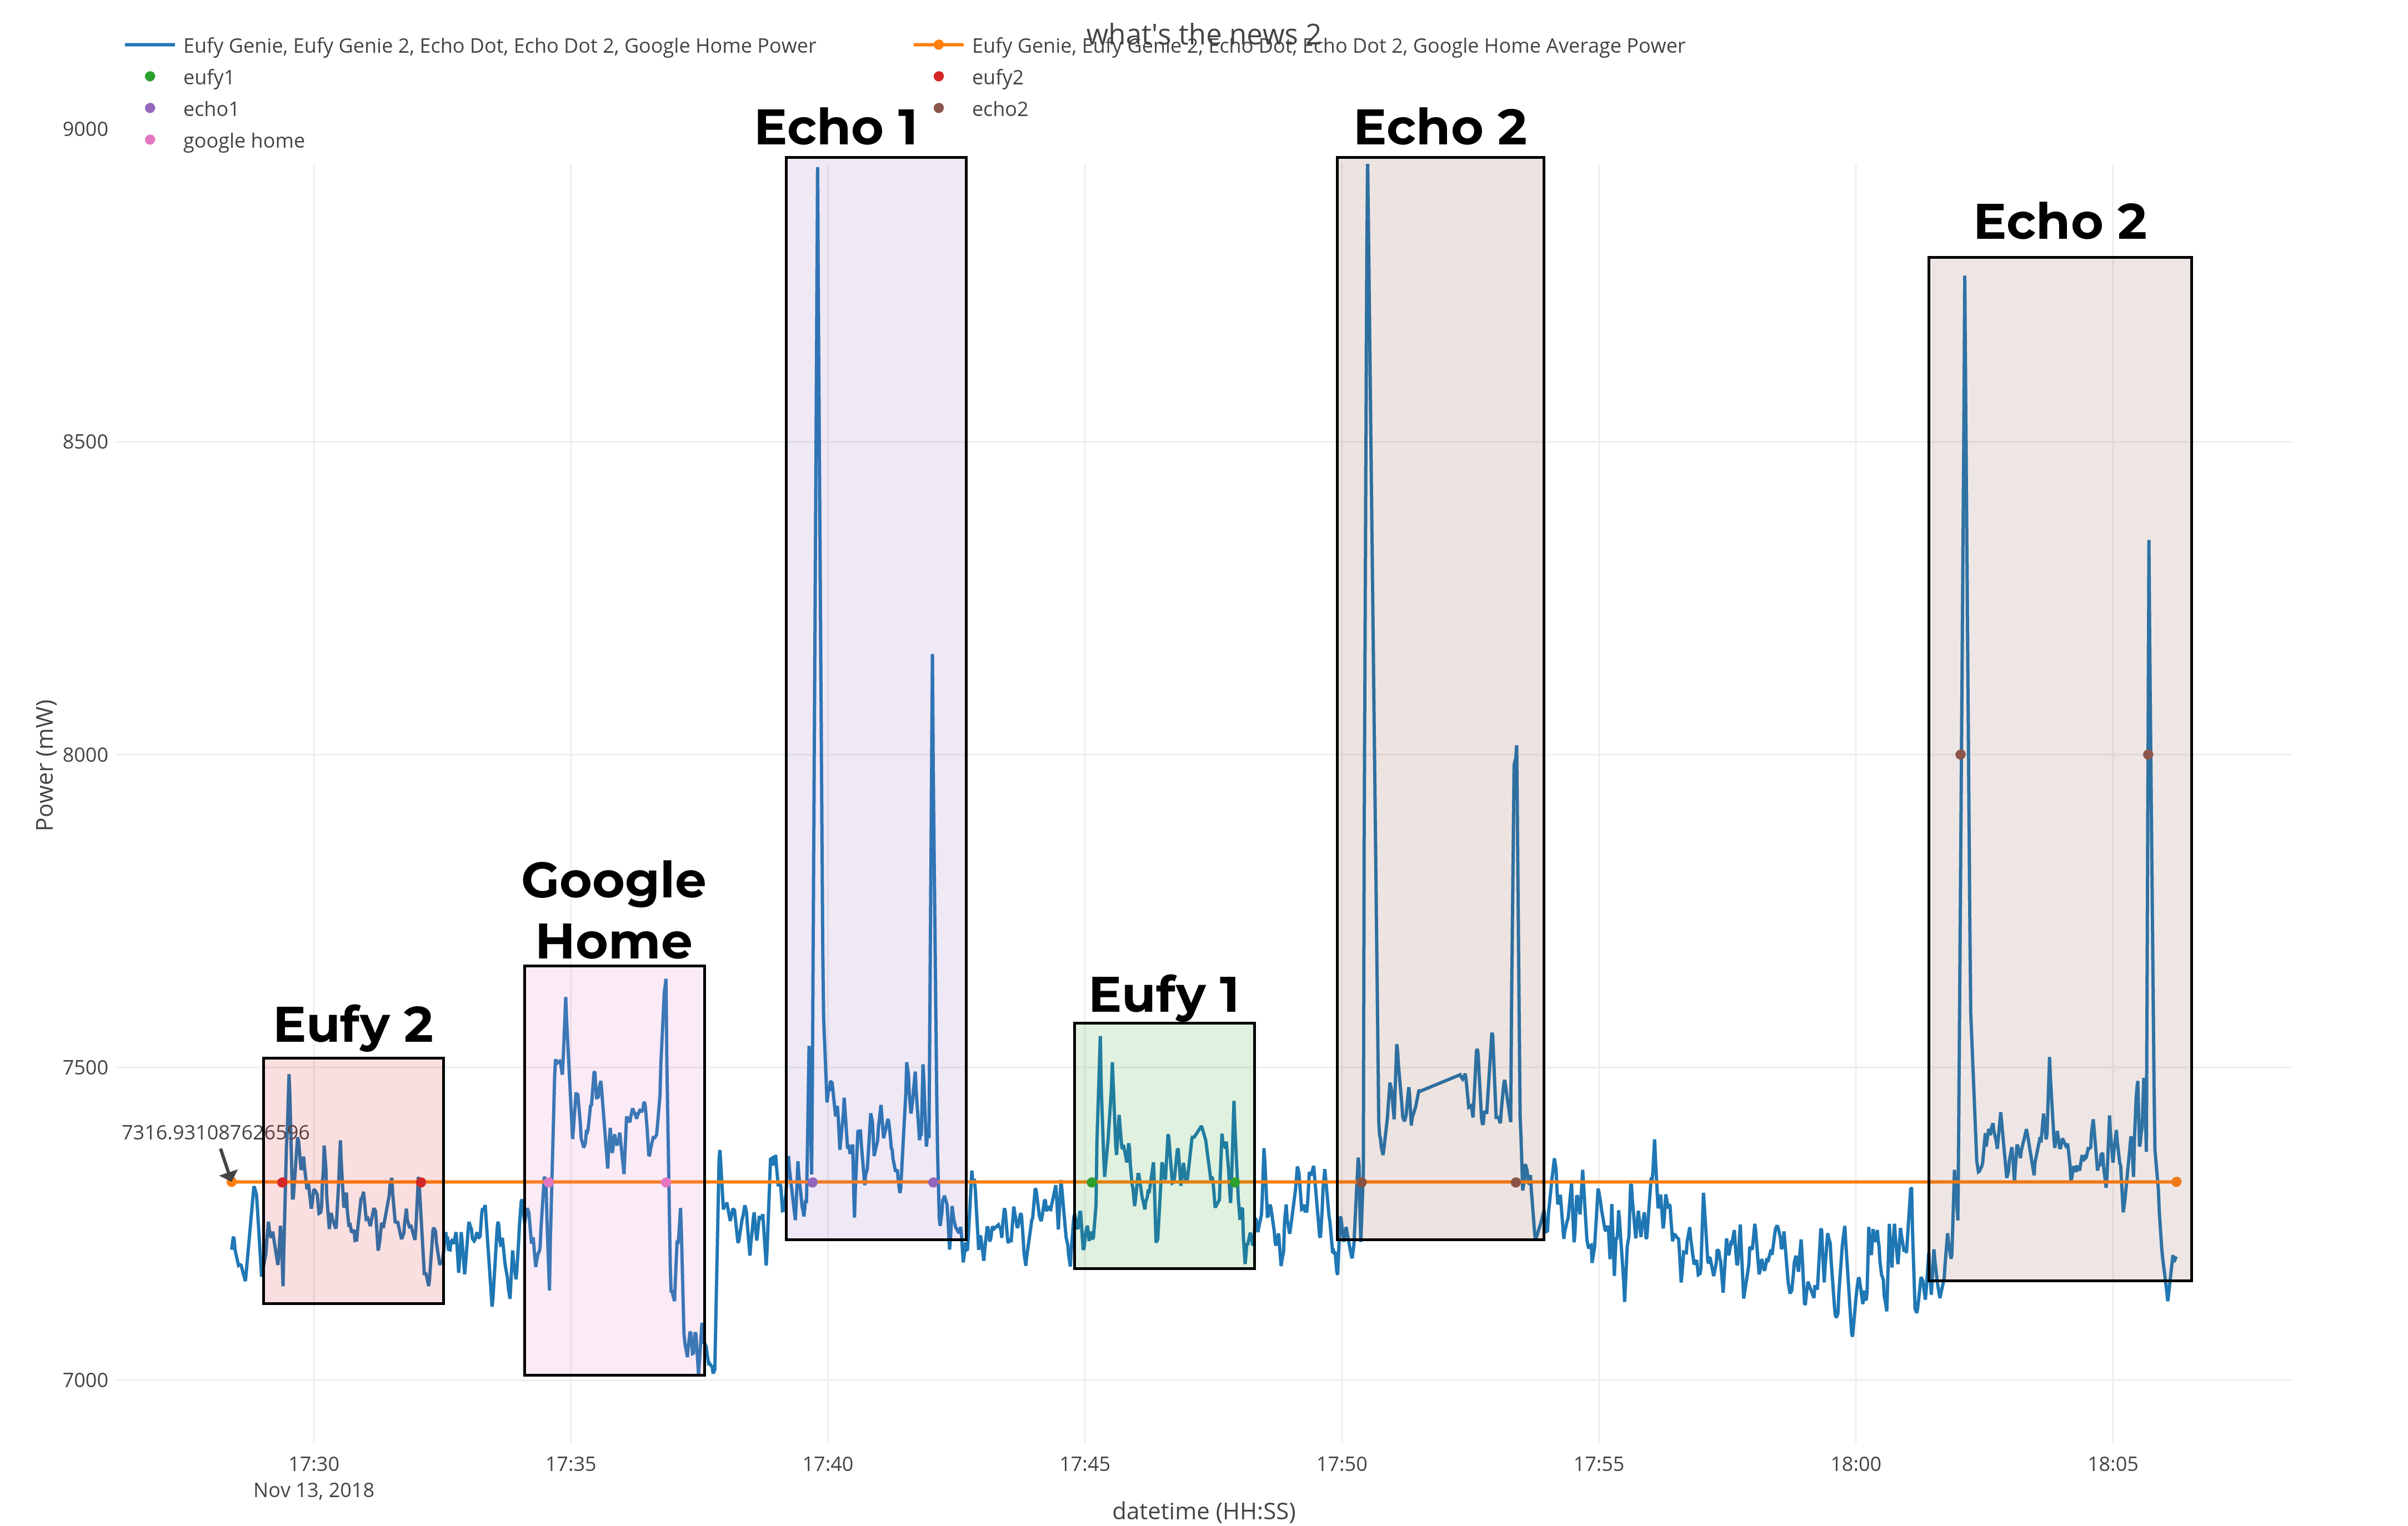
\includegraphics[width=1\textwidth]{figures/mixedNewsSum.png}
  \caption{5 Smart Speakers Power Summed Up. Queried each device for the
  news.}
  \label{fig:mixedNewsSum}
\end{figure}

The next graph, \ref{fig:bestBballSum}, shows the smart speakers when asked for the best basketball player. The annotation scheme is the same as before. Each smart speaker is queried for the best basketball player in consecutive order four times. Similar to before, the Eufy has a power spike of 420 mW peak to peak, the Google Home has a power Spike of 720 mW, and the Echo Dot has a power spike of 2180 mW.

When looking at graph \ref{fig:bestBballSum}, there is a power spike that is unaccounted for in correspondence to the event log at 18:12. We made a query, invoking all other power spikes but we did not do anything for the power spike at 18:12 that is higher than the other Eufy power spikes shown in first half of figure \ref{fig:bestBballSum} up to 18:24.

To figure what the power spike at 18:12 is, we separated the graphs into individual power traces as shown in figure \ref{fig:bestBballSeperate}. From this graph, the power spike at 18:12 is attributed to the Echo Dot 2 because it is the only trace with a spike occuring. We then looked at the individual network usage for each of these devices in this time frame as shown in figure \ref{fig:bestBballNetwork}. At 18:12, there is no significant network usage.

We had no conclusive evidence to decide what the power spike means. But in speculation, because there is no network usage during this time, we do not think the Echo Dot was doing anything data recording, listening, or was activated. We believe that the computer was covering the Echo Dot, but is briefly moved, exposing the Echo Dot to more light, thus causing the LEDs to brighten.

\begin{figure}[H]
  \centering
  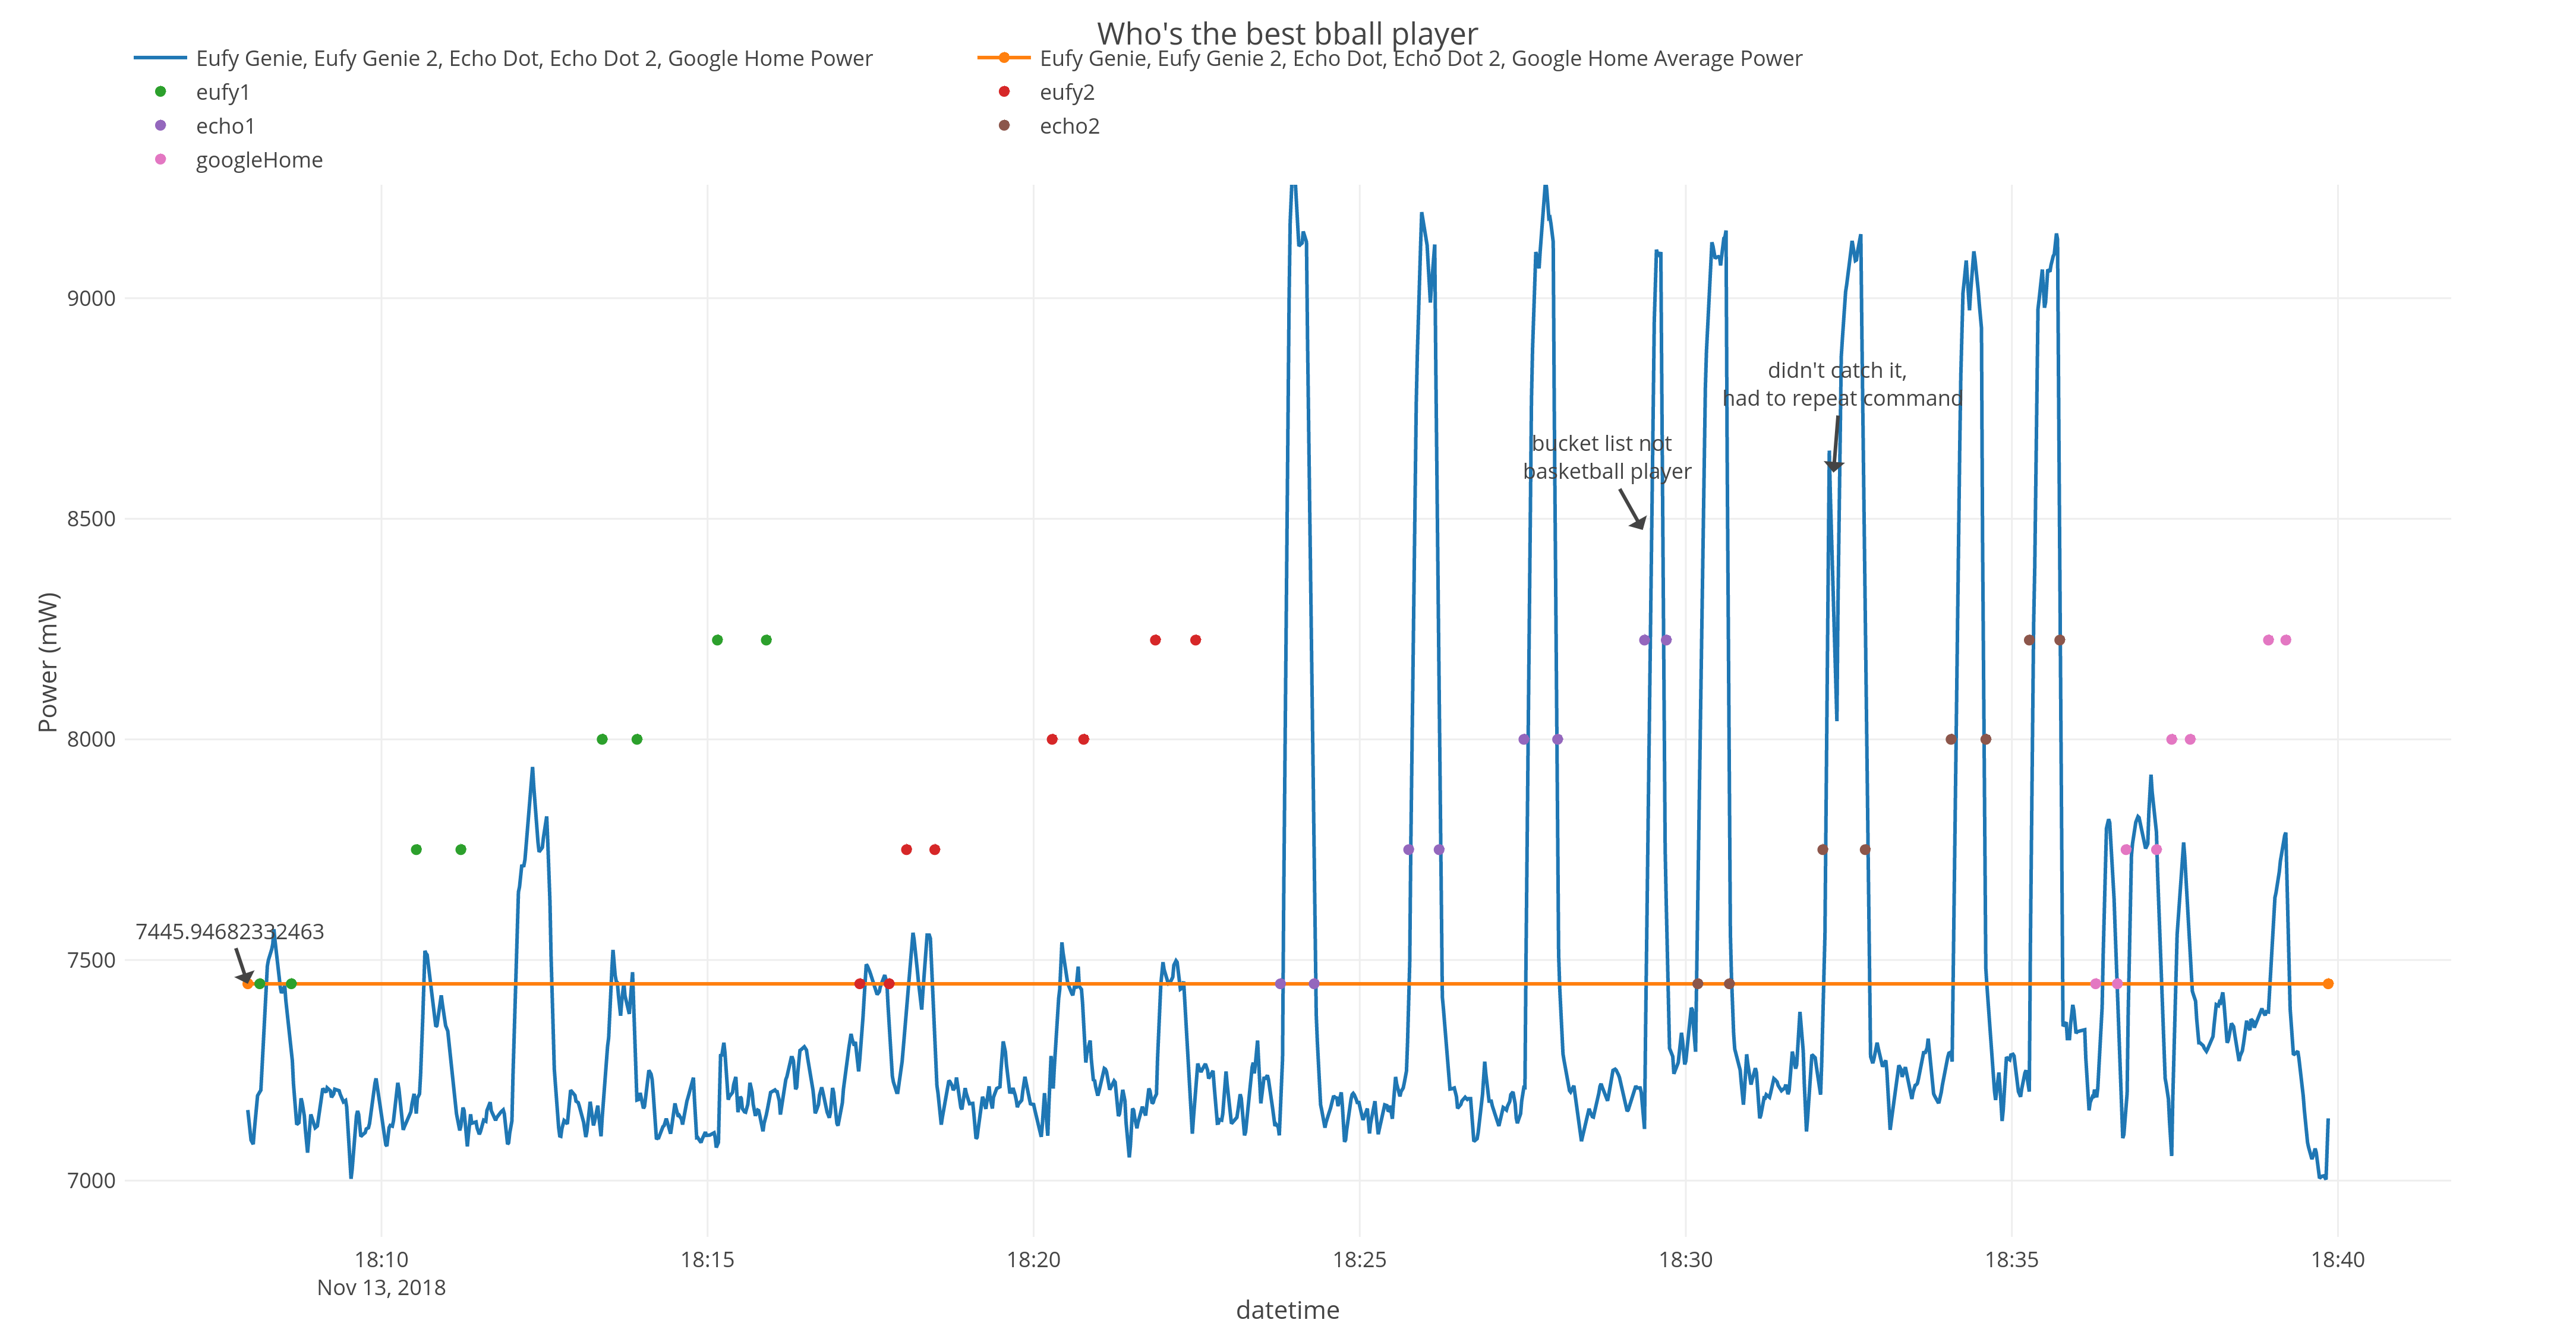
\includegraphics[width=1\textwidth]{figures/bestBballSum.png}
  \caption{5 Smart Speakers Power Summed Up. Queried each device for the
  best basketball player.}
  \label{fig:bestBballSum}
\end{figure}

\begin{figure}[H]
  \centering
  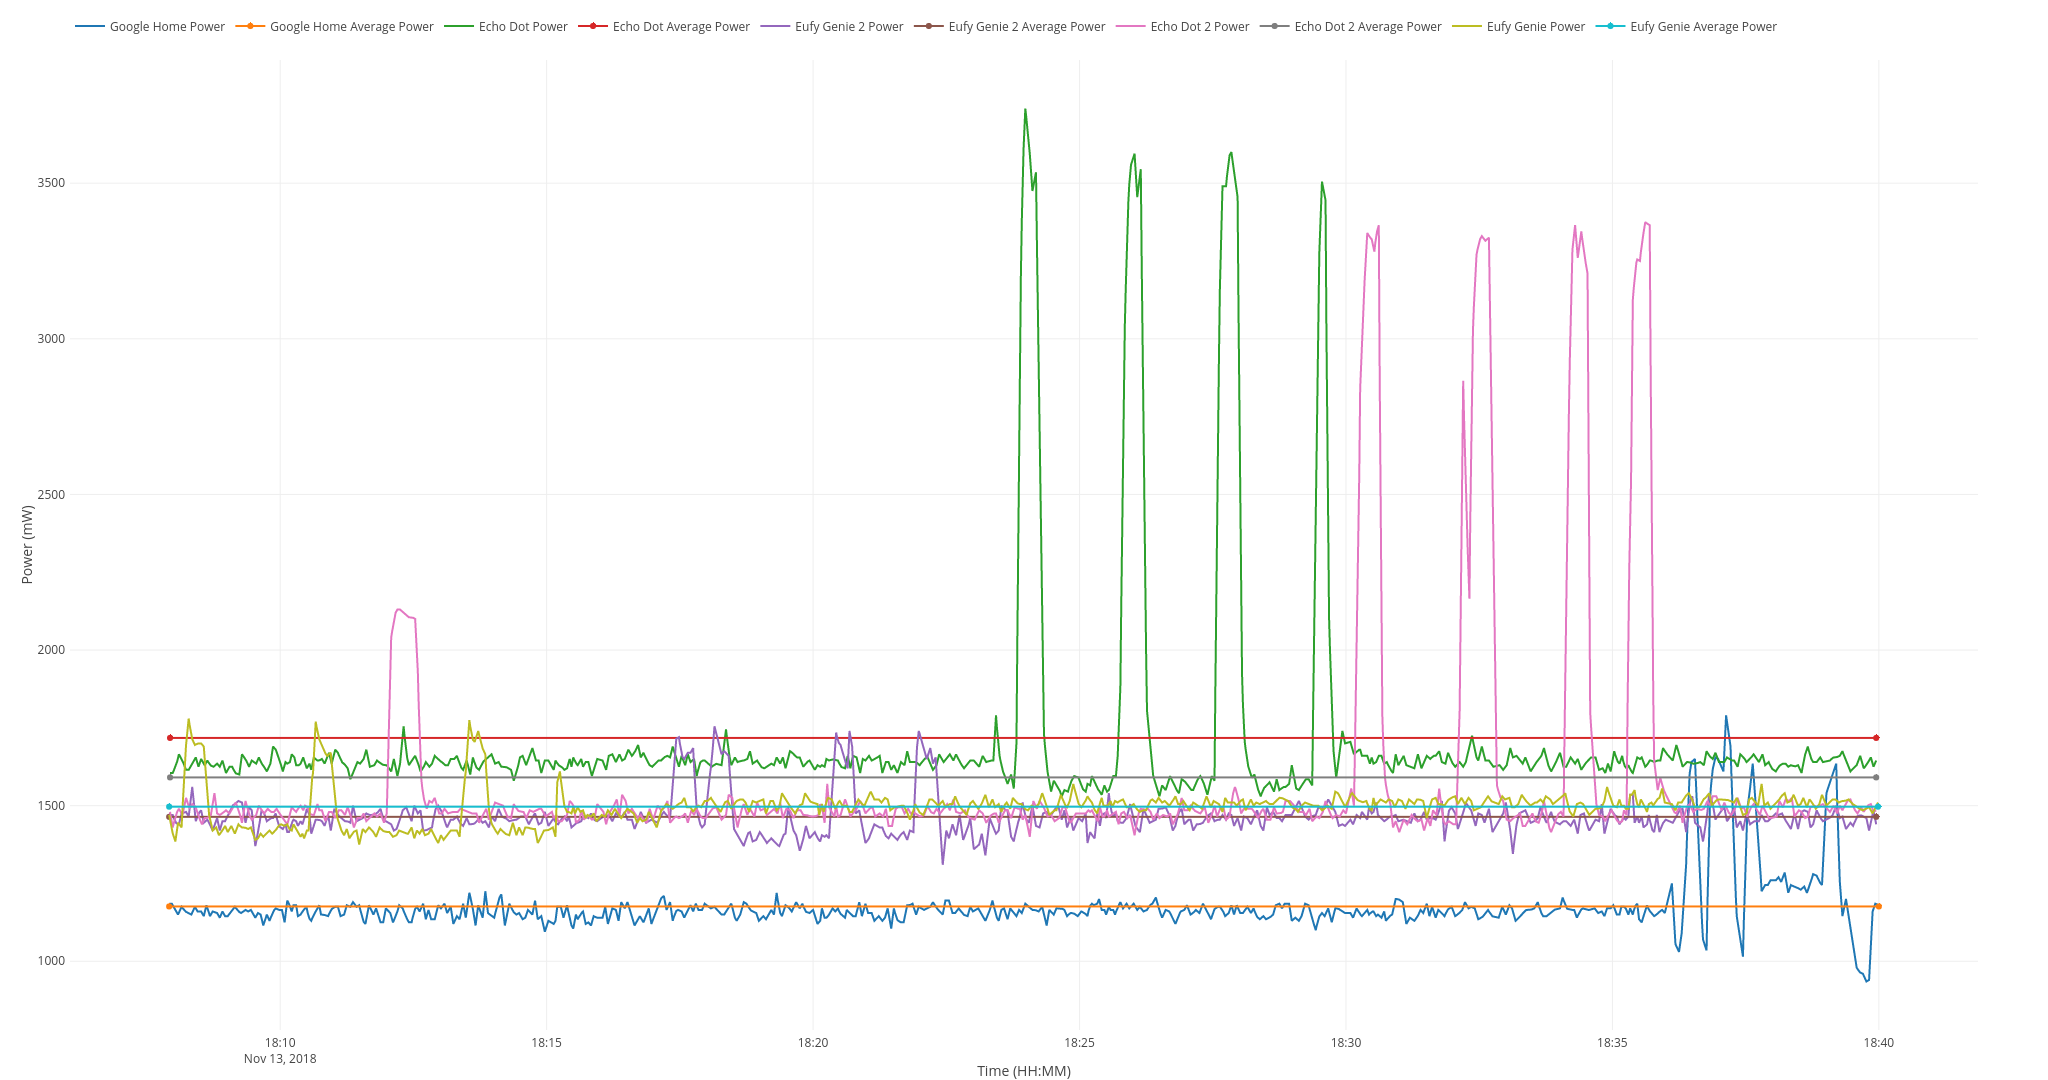
\includegraphics[width=1\textwidth]{figures/bestBballSeperate.png}
  \caption{5 Smart Speakers Power Usage over time. Queried each device for the
  best basketball player.}
  \label{fig:bestBballSeperate}
\end{figure}

\begin{figure}[H]
  \centering
  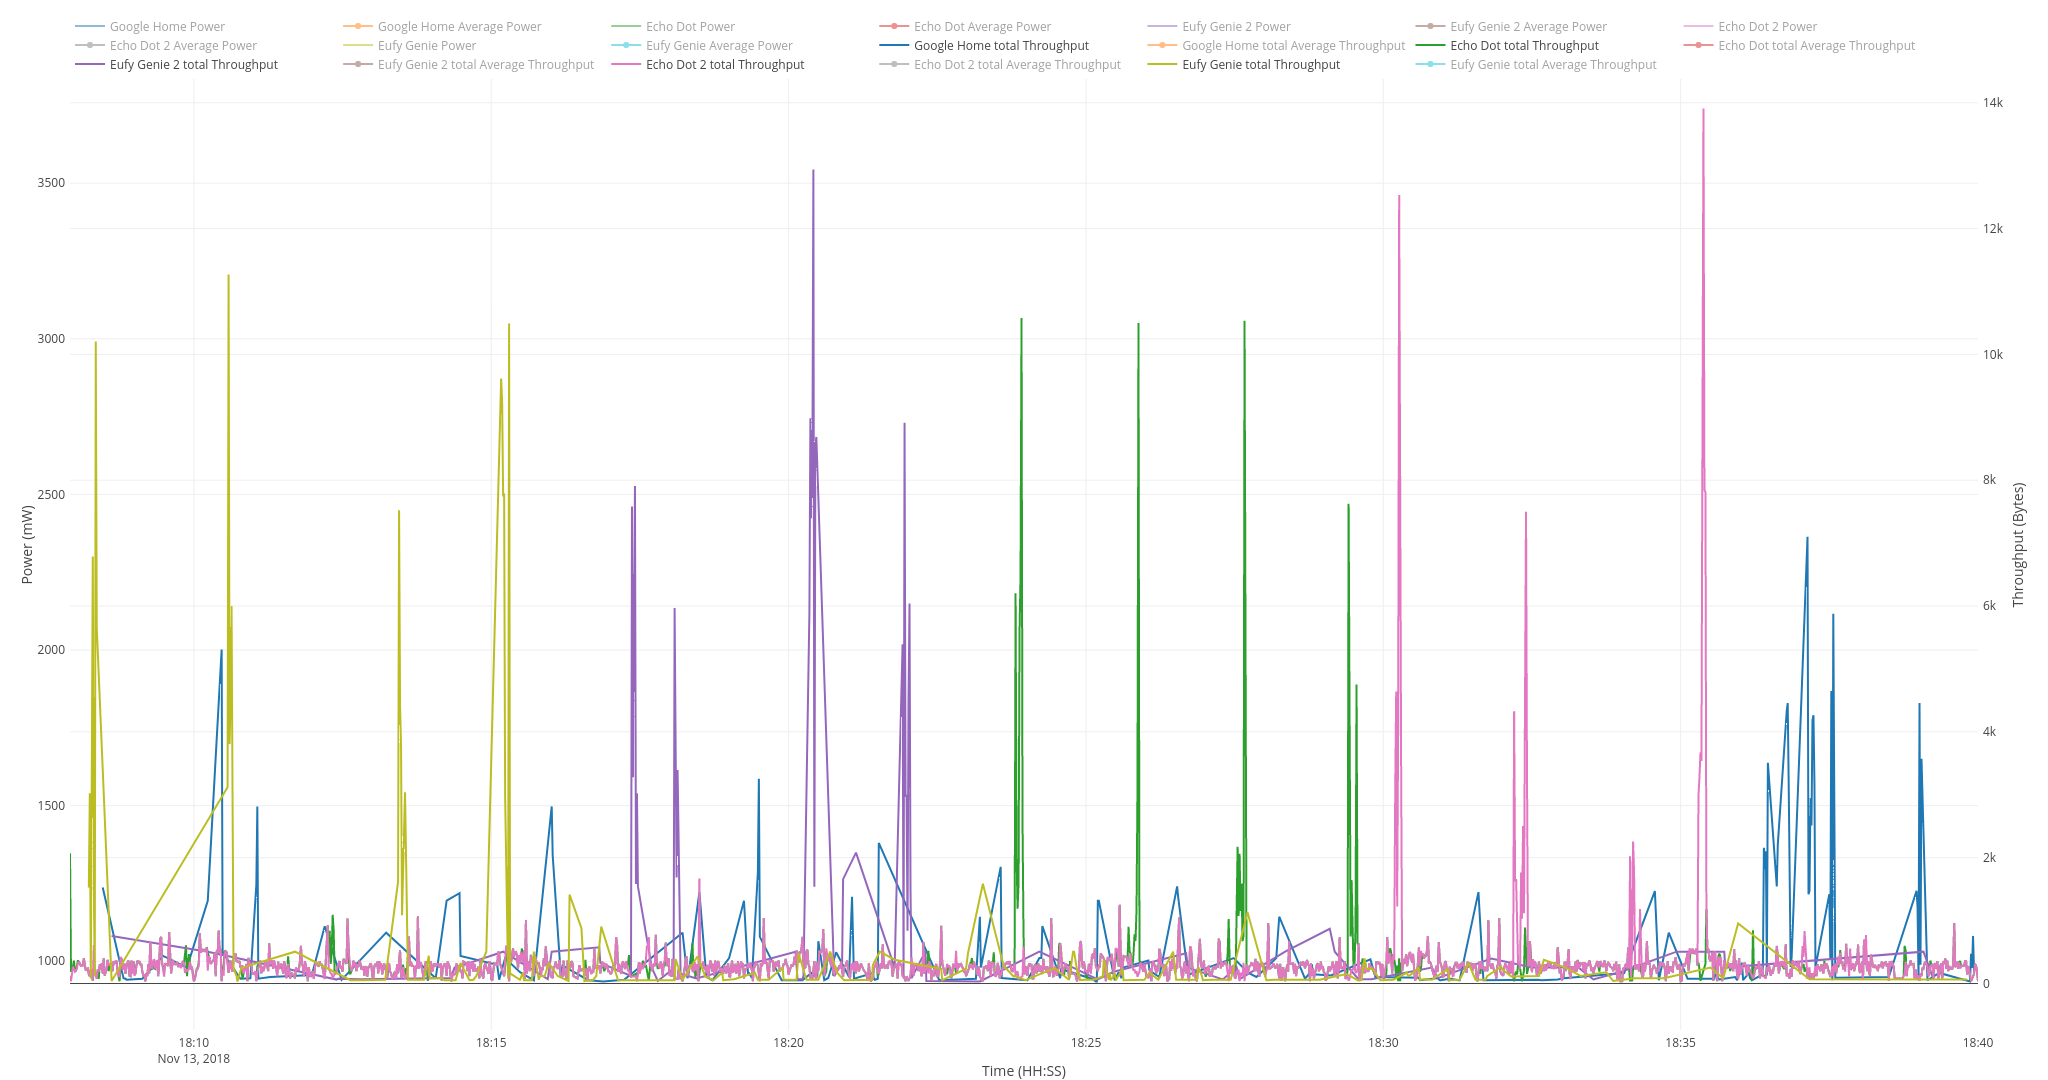
\includegraphics[width=1\textwidth]{figures/bestBballNetwork.png}
  \caption{5 Smart Speakers Network throughput over time. Queried each device for the best basketball player.}
  \label{fig:bestBballNetwork}
\end{figure}

The power spike information for each query type (``what's the weather'' ``what's the news'', ``who's the best basketball player'') is shown below in figure \ref{fig:spikeVoltages}. From figures \ref{fig:weatherSum}, \ref{fig:mixedNewsSum}, and \ref{fig:bestBballSum} there is always a characteristic power spike that occurs at the beginning of a command for each device. This bar graph also includes the total average spike height for each command for all three of these commands. The black line at the top of each bar shows the standard deviation. Averaging peak to peak voltage spikes for each device shows the Eufy Genie with a 390 mW spike with 36.1 mW standard deviation, the Google Home with a 606.7 mW spike with 110 mW standard deviation, the Echo Dot with a 2026.7 mW spike with 149.89 mW standard deviation.

From figure \ref{fig:spikeVoltages}, we can determine what device model is being used if it is within those thresholds. The models with multiple units are consistent with each other. From this, we conclude it is possible to determine a device model from visual examination of its power usage. This is our first step to testing our hypotheses that it is possible to see what devices are in use from analysis of someone's power line.

\begin{figure}[H]
  \centering
  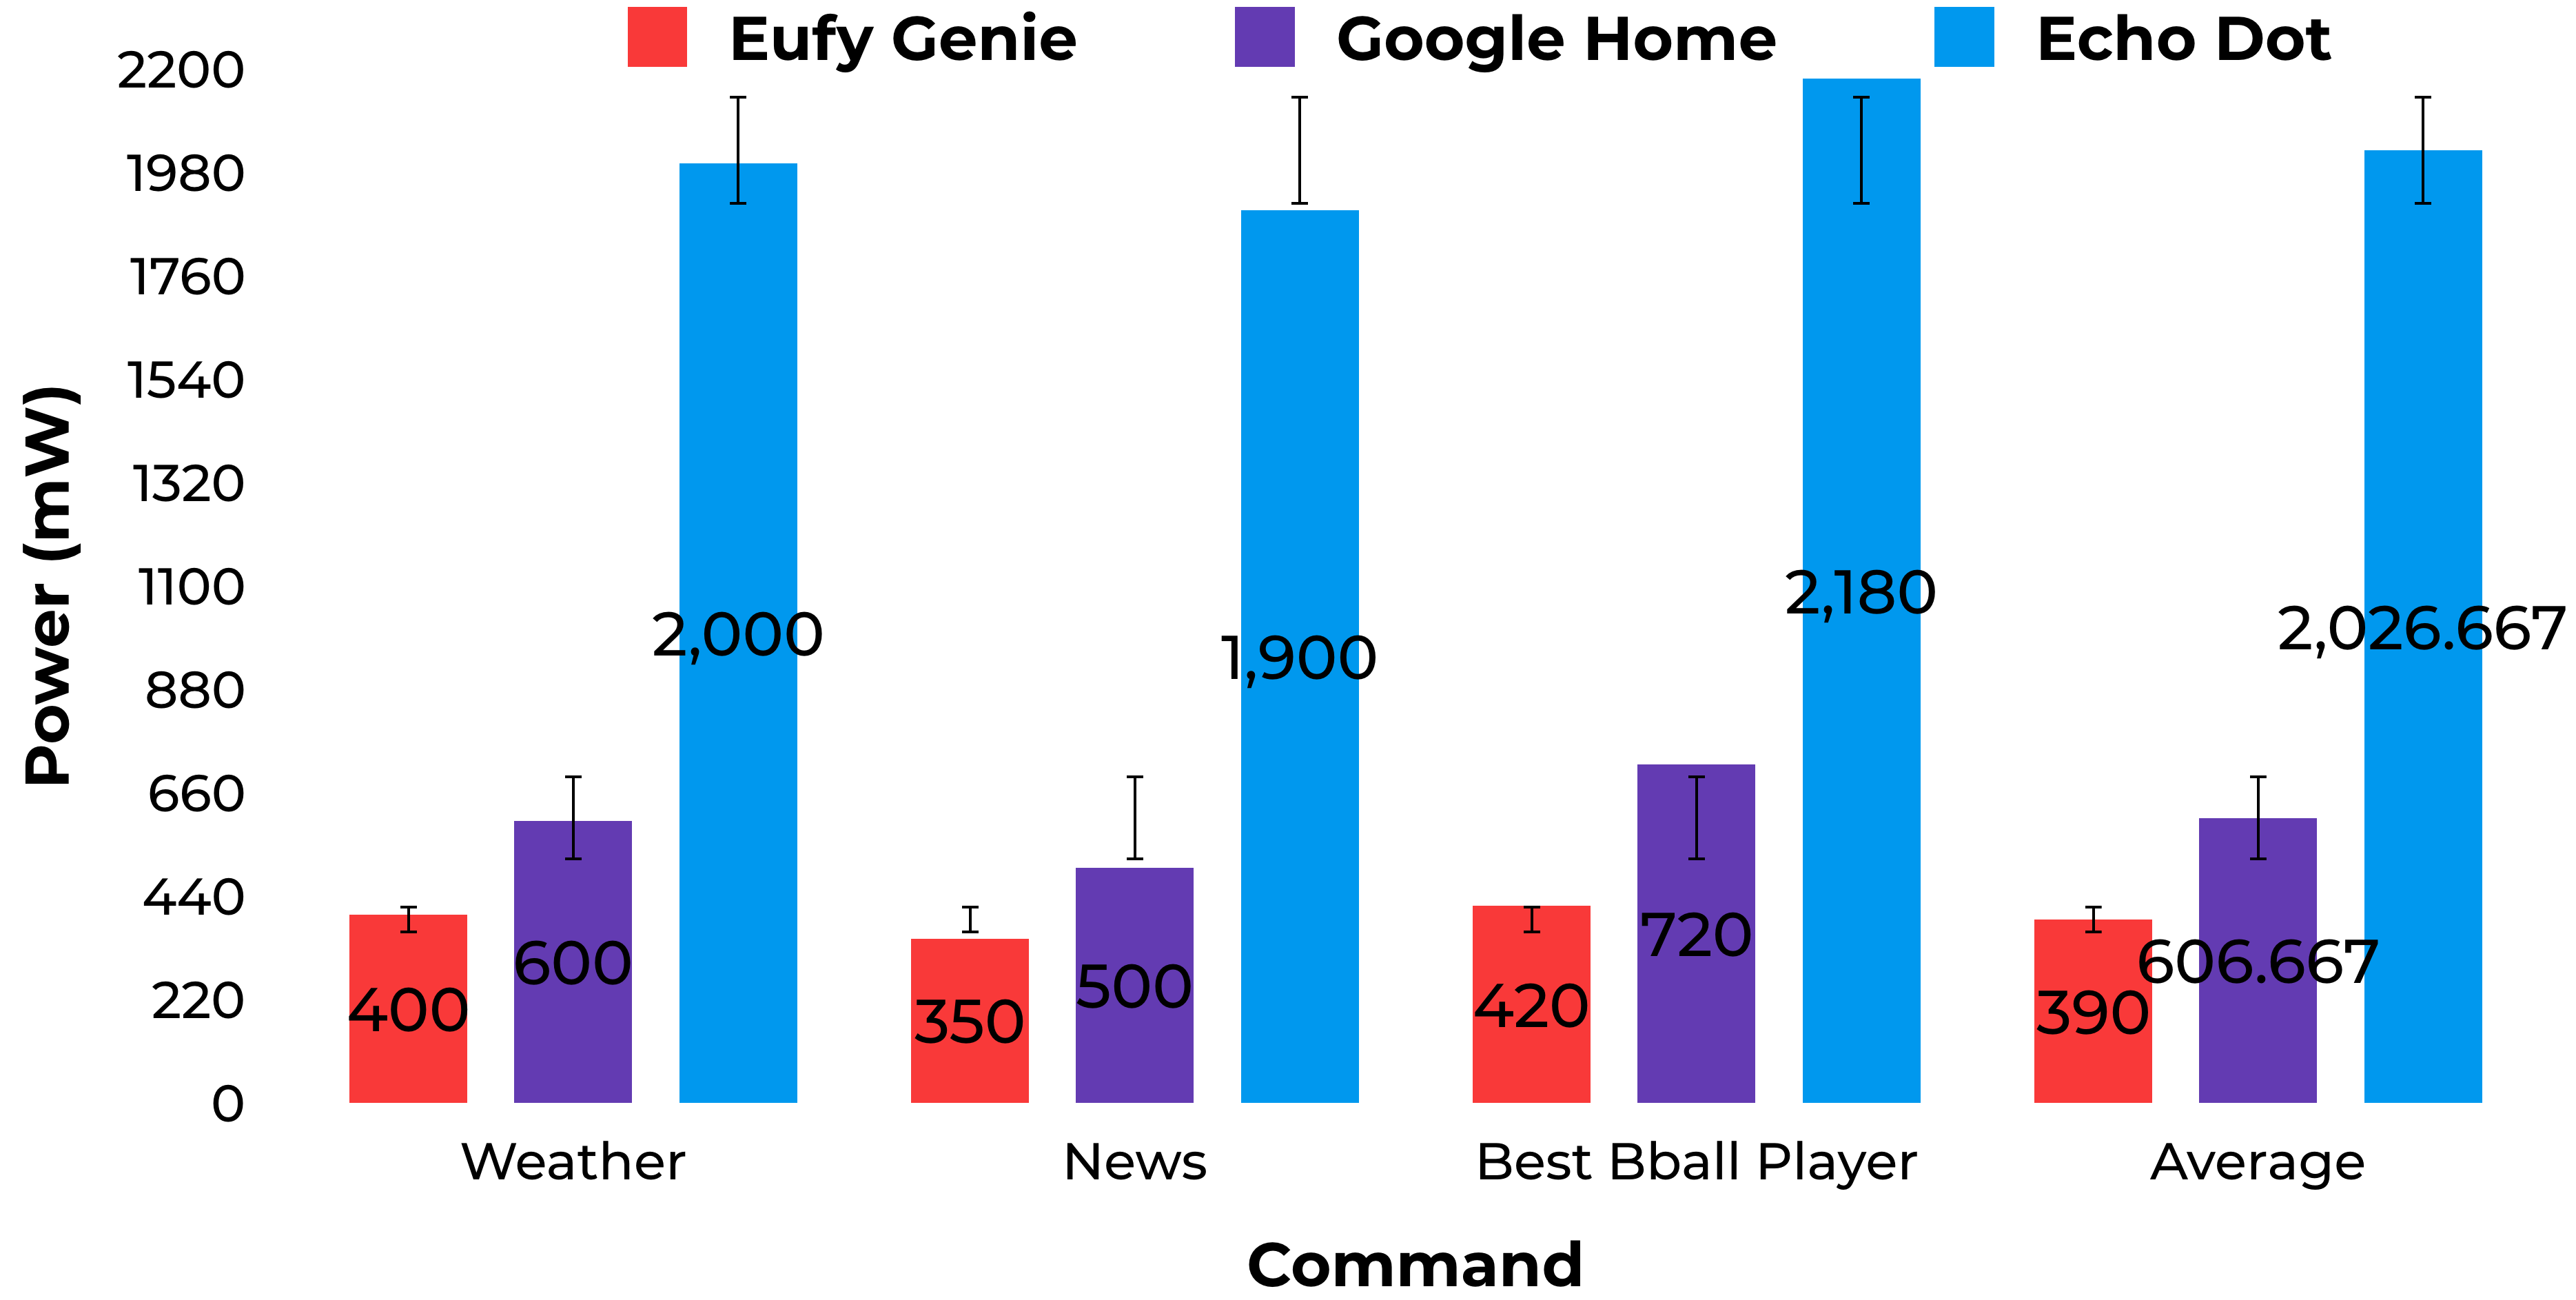
\includegraphics[width=1\textwidth]{figures/spikeVoltages.png}
  \caption{Spike summary of for each query.}
  \label{fig:spikeVoltages}
\end{figure}

But in a real house, there are more than just 5 smart speakers on a power line. The next step is to add noise from high power devices to see if it is still possible to visually determine the device in use from power spikes \ref{sumPowerGraphWithNoise}.

\section{Summed Power Graph With Noise}
\label{sumPowerGraphWithNoise}
In this section, we introduce noise into the system so that we can determine if the power spike from each smart speaker is still discernible within a summed power graph when we add high power devices.

In each subsection, there are three traces. The first trace (blue trace) is the summed power usage of our five smart speakers (2 Echo Dots, 2 Eufy Genies, 1 Google Home) when asked for the best basketball player 4 times. This is the same trace as shown in \ref{fig:bestBballSum}. is the power usage over time for a high power device. The second trace (purple trace) is the power usage of a high power device. This trace is the added noise. It maps to various devices as we switch them out. The third trace (red trace) is the sum of both trace 1 and 2. It is the power usage of the smart speakers in the blue trace with the noise from the device in the purple trace.

There x-axis is the time elapsed in seconds. There is no time vecause the smart speaker trace was taken at a seperate time from when the noise trace was taken. The y-axis is the power used by each device over time.

Below, in figure \ref{fig:fanIdleSeperate}, is an example of the traces used seperately. Taking the blue trace (smart speaker power usage) and the purple trace (noise introducing device) the summed up graph will result in the red trace (total power usage). This is shown seperately at first, but will be summed together for the rest of the paper so that the scale of the noise can be understood.

\begin{figure}[H]
  \centering
  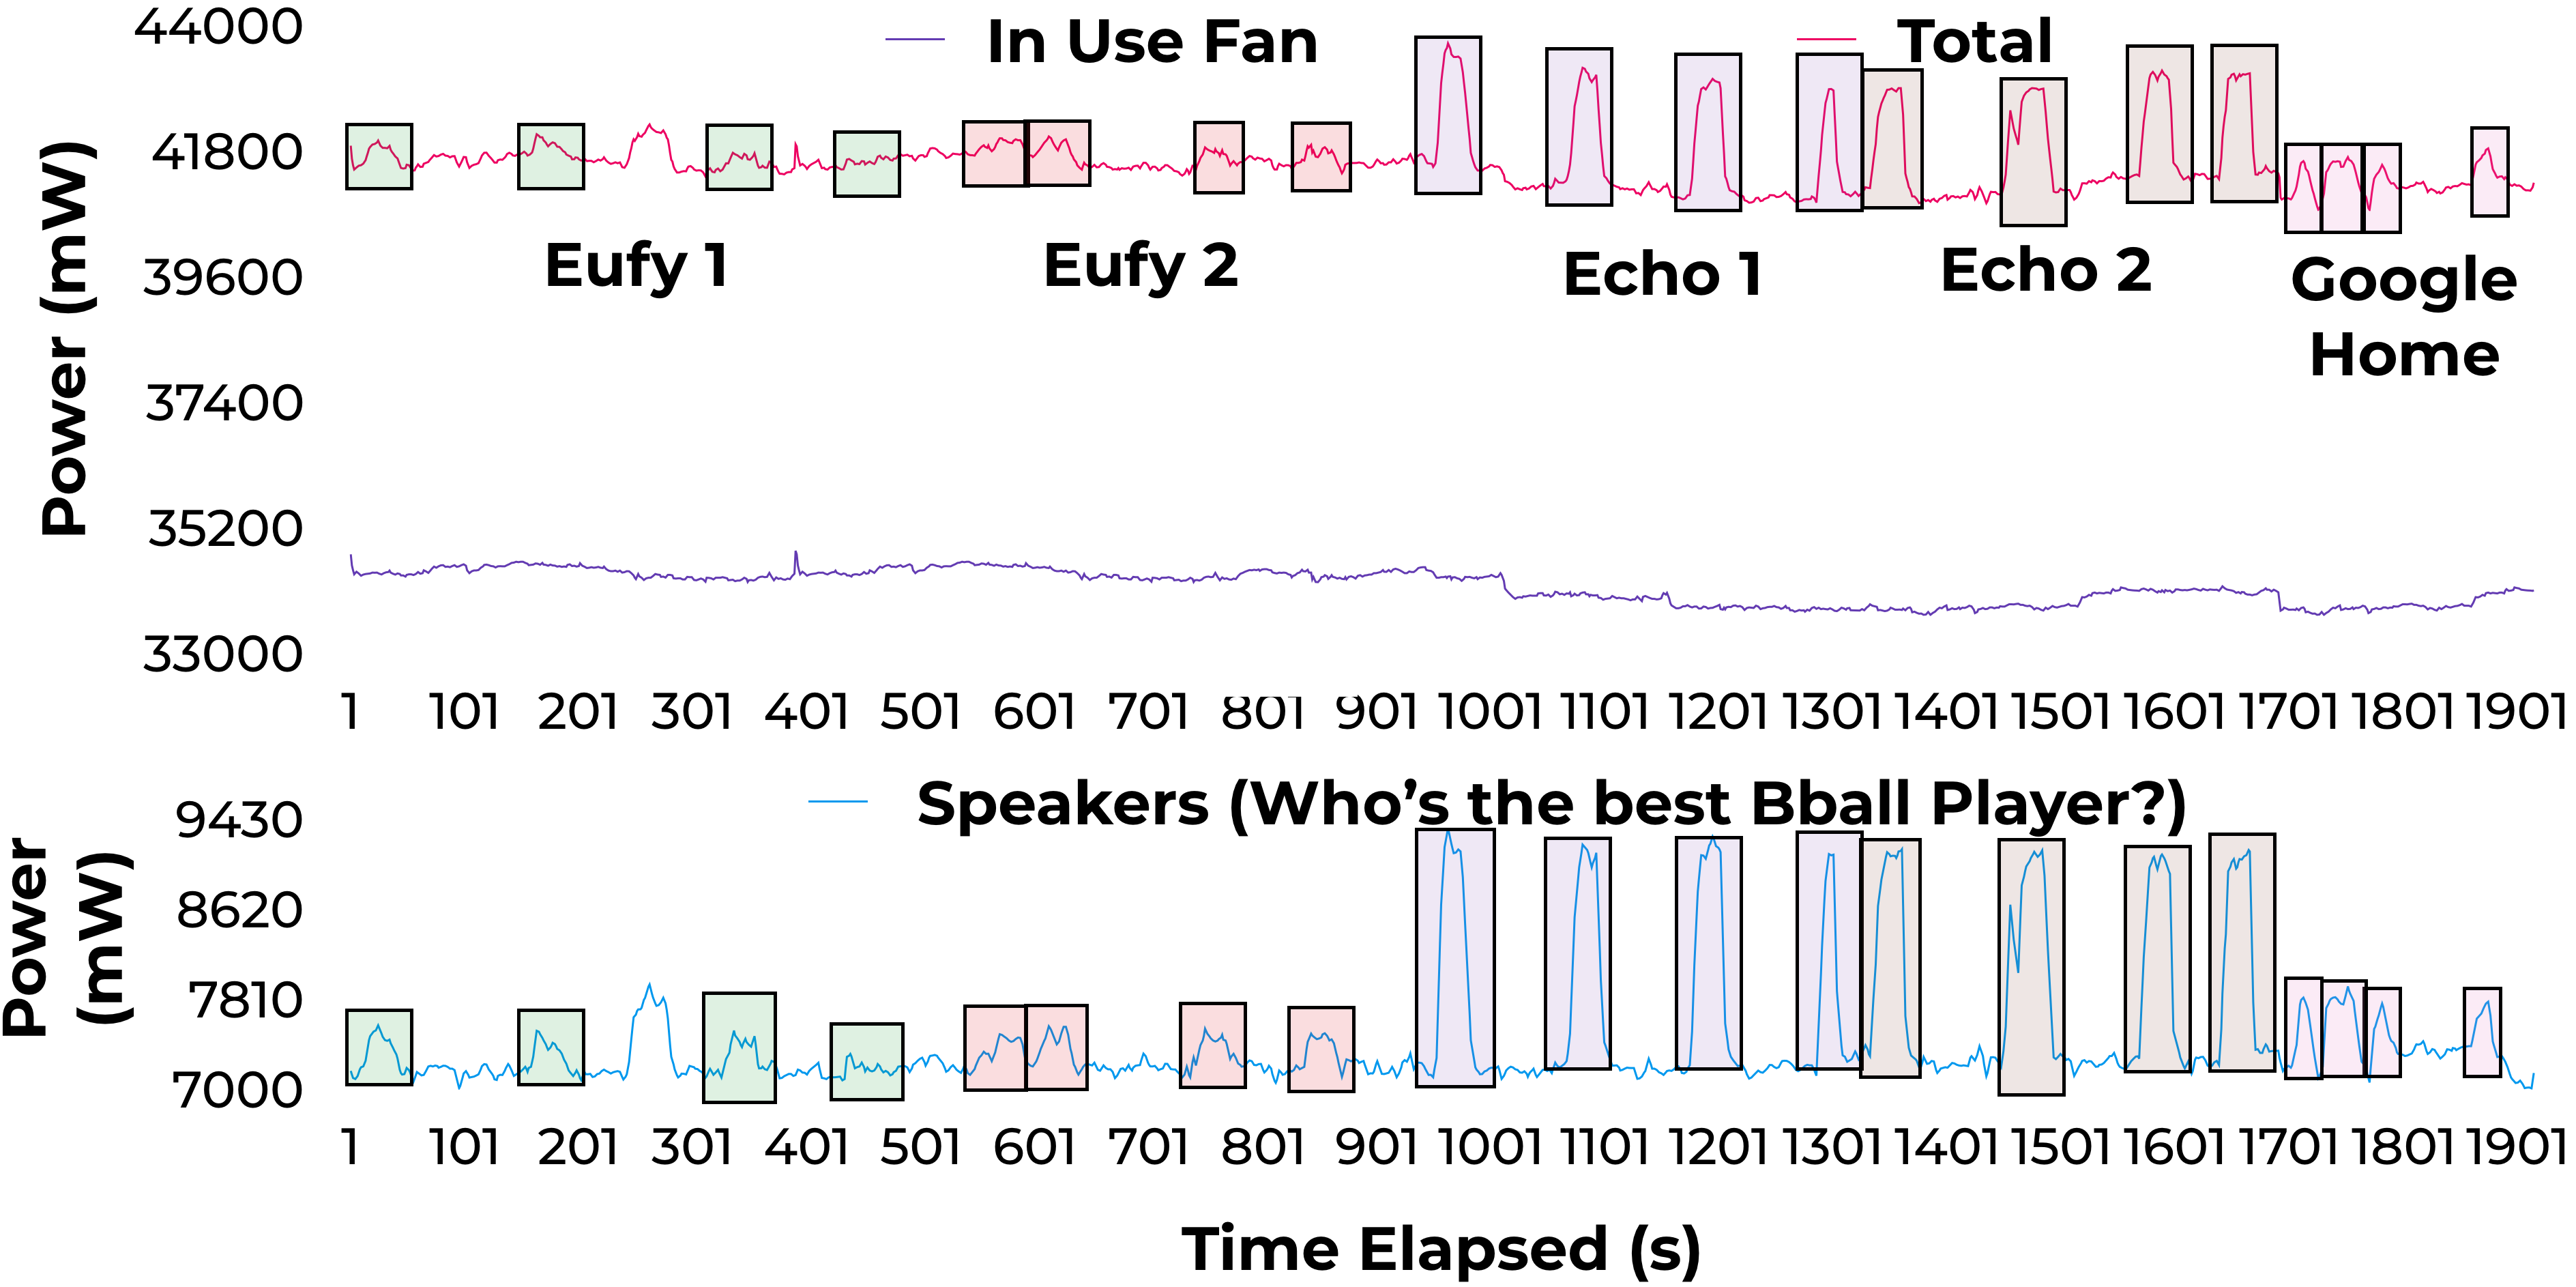
\includegraphics[width=1\textwidth]{figures/inUseFanNoiseSeperate.png}
  \caption{Idle Fan with figure \ref{fig:bestBballSum} trace shown seperately.}
  \label{fig:fanIdleSeperate}
\end{figure}

Below, we display the smart speaker trace with a PC (Intel NUC), fan, refrigerator, or microwave. Figures \ref{fig:fanIdleSeperate}, \ref{fig:fanIdle}, \ref{fig:uWaveIdle}, \ref{fig:fridgeIdle}, \ref{fig:nucIdle}, and \ref{fig:allIdleNoise} begin with noise from devices while idle or during steady power usage to set a baseline. Then figures \ref{fig:uWaveInUse}, \ref{fig:fridgeInUse}, and \ref{fig:nucInUse} show noise from devices while in use, introducing noise that make visual detection of smart speakers most difficult.

In figures \ref{fig:fanIdle}, \ref{fig:uWaveIdle}, \ref{fig:fridgeIdle}, and \ref{fig:nucIdle}, the power spikes from the smart speakers can still be seen. Visually, the Echo Dot power spike is clearly seen in red trace for each graph. The power spikes for the Google Home and Eufy Genie are less visible but can still be seen. Especially when zoomed in as shown in figure \ref{fig:allIdleNoise} where the smart speaker trace is removed.

\begin{figure}[H]
  \centering
  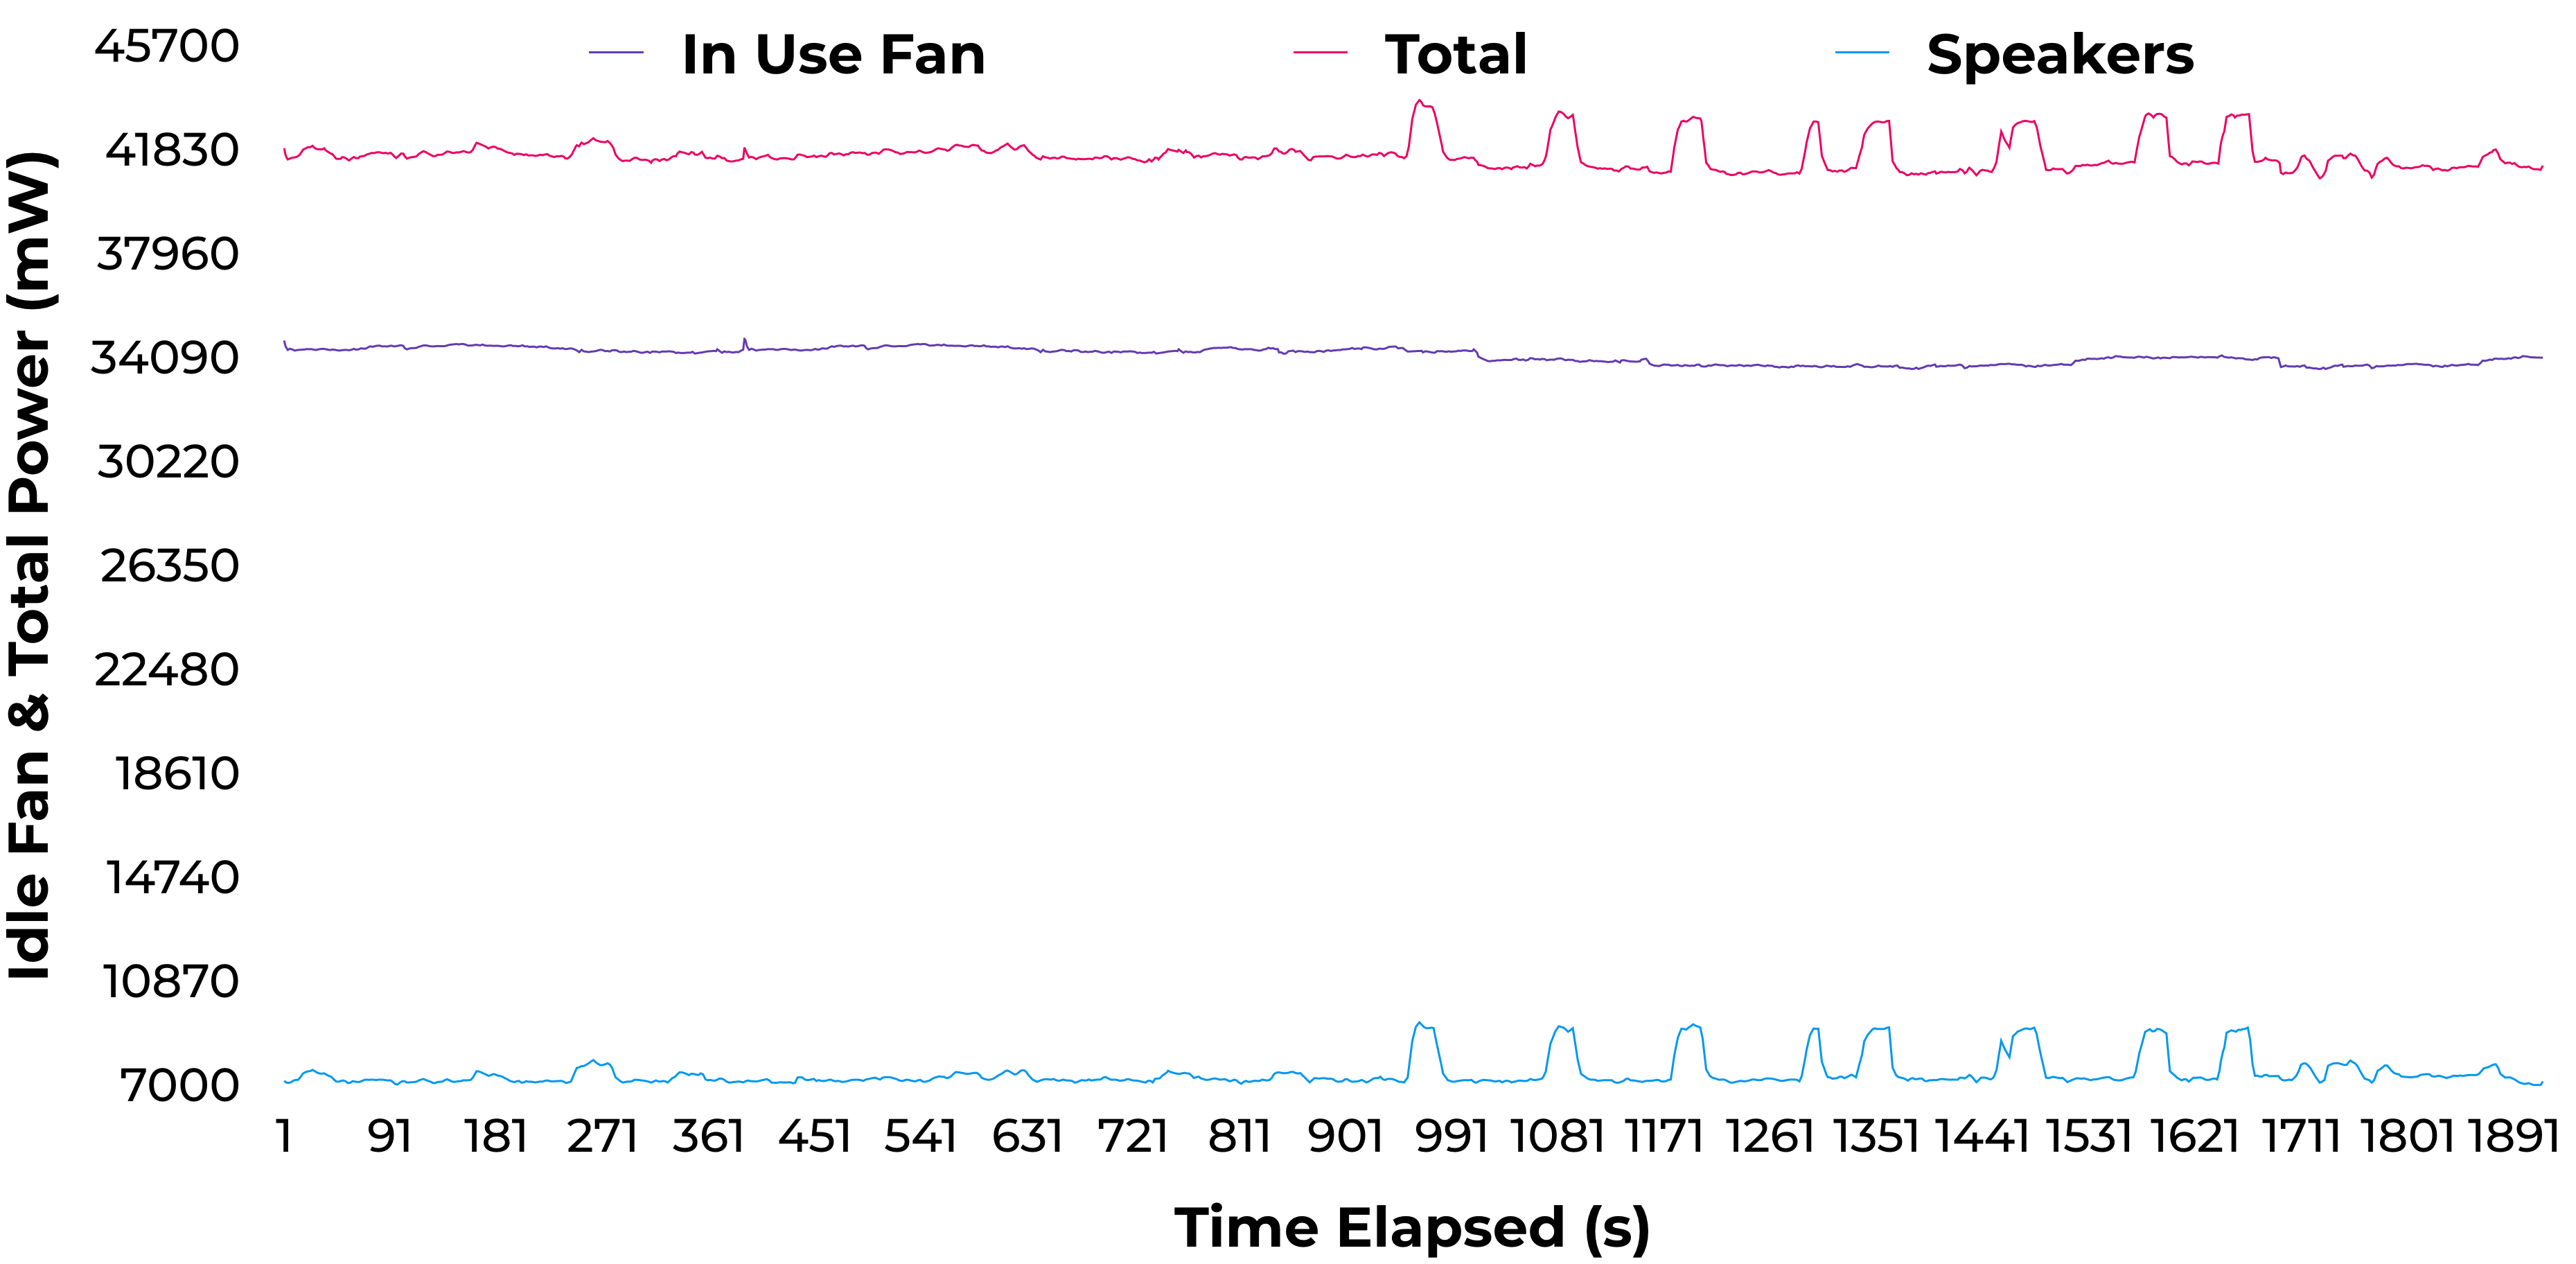
\includegraphics[width=1\textwidth]{figures/inUseFanNoise.png}
  \caption{Idle Fan with figure \ref{fig:bestBballSum} trace.}
  \label{fig:fanIdle}
\end{figure}

\begin{figure}[H]
  \centering
  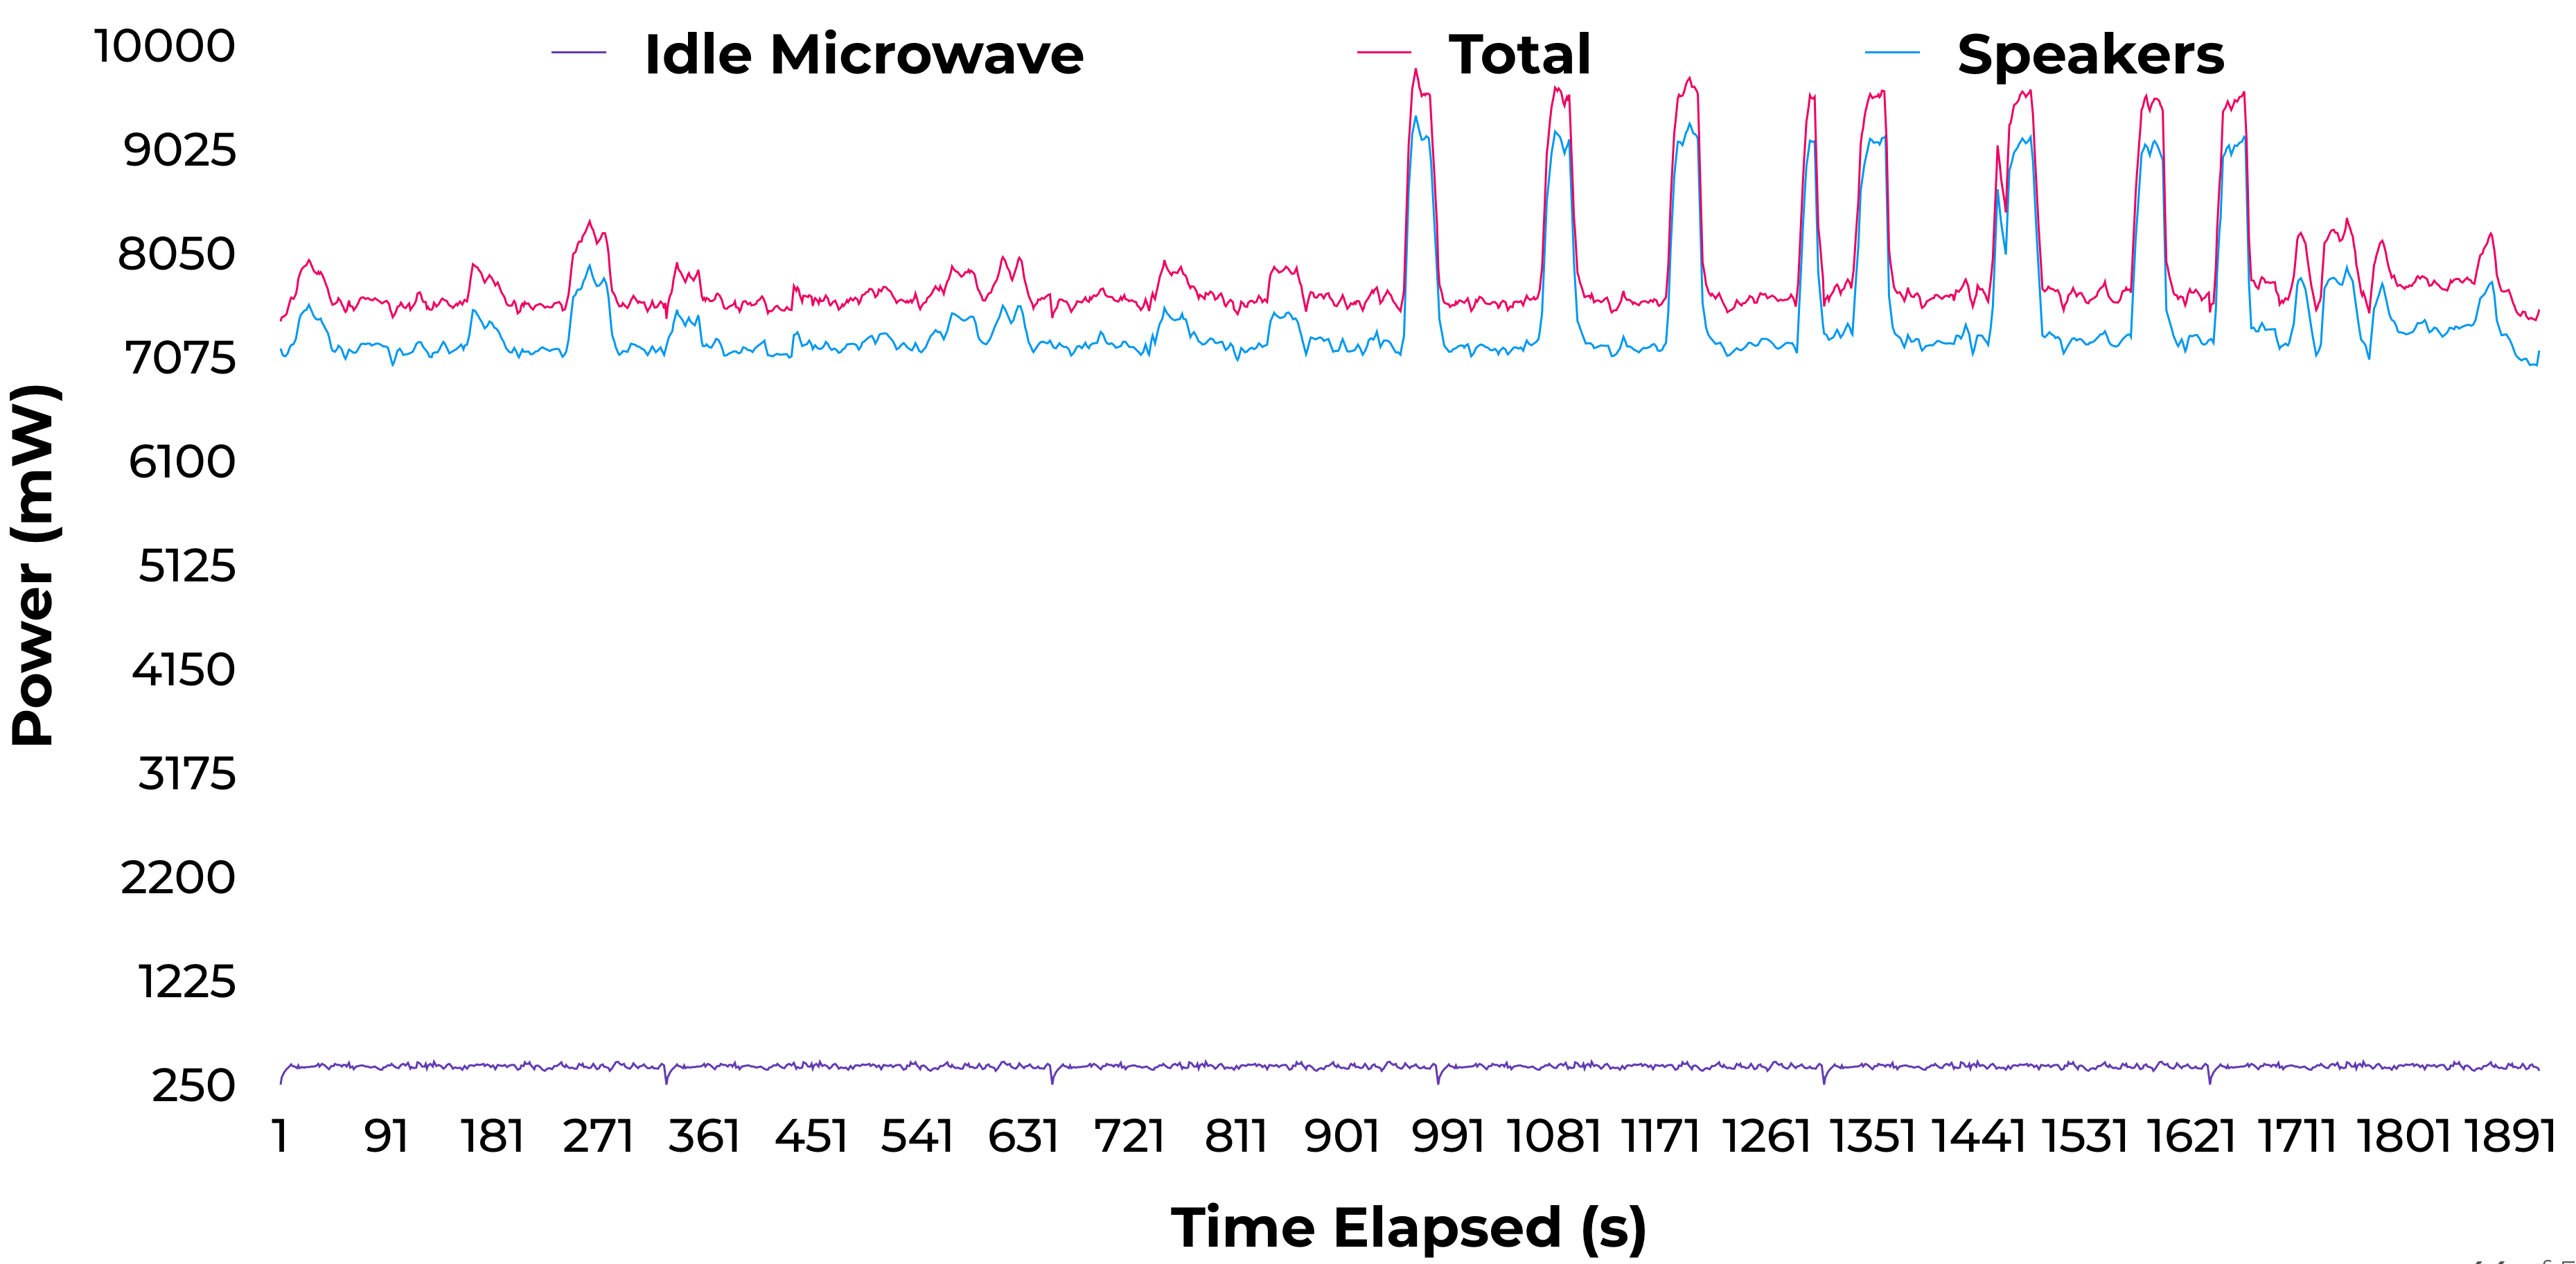
\includegraphics[width=1\textwidth]{figures/idleuWaveNoise.png}
  \caption{Idle microwave with figure \ref{fig:bestBballSum} trace.}
  \label{fig:uWaveIdle}
\end{figure}

\begin{figure}[H]
  \centering
  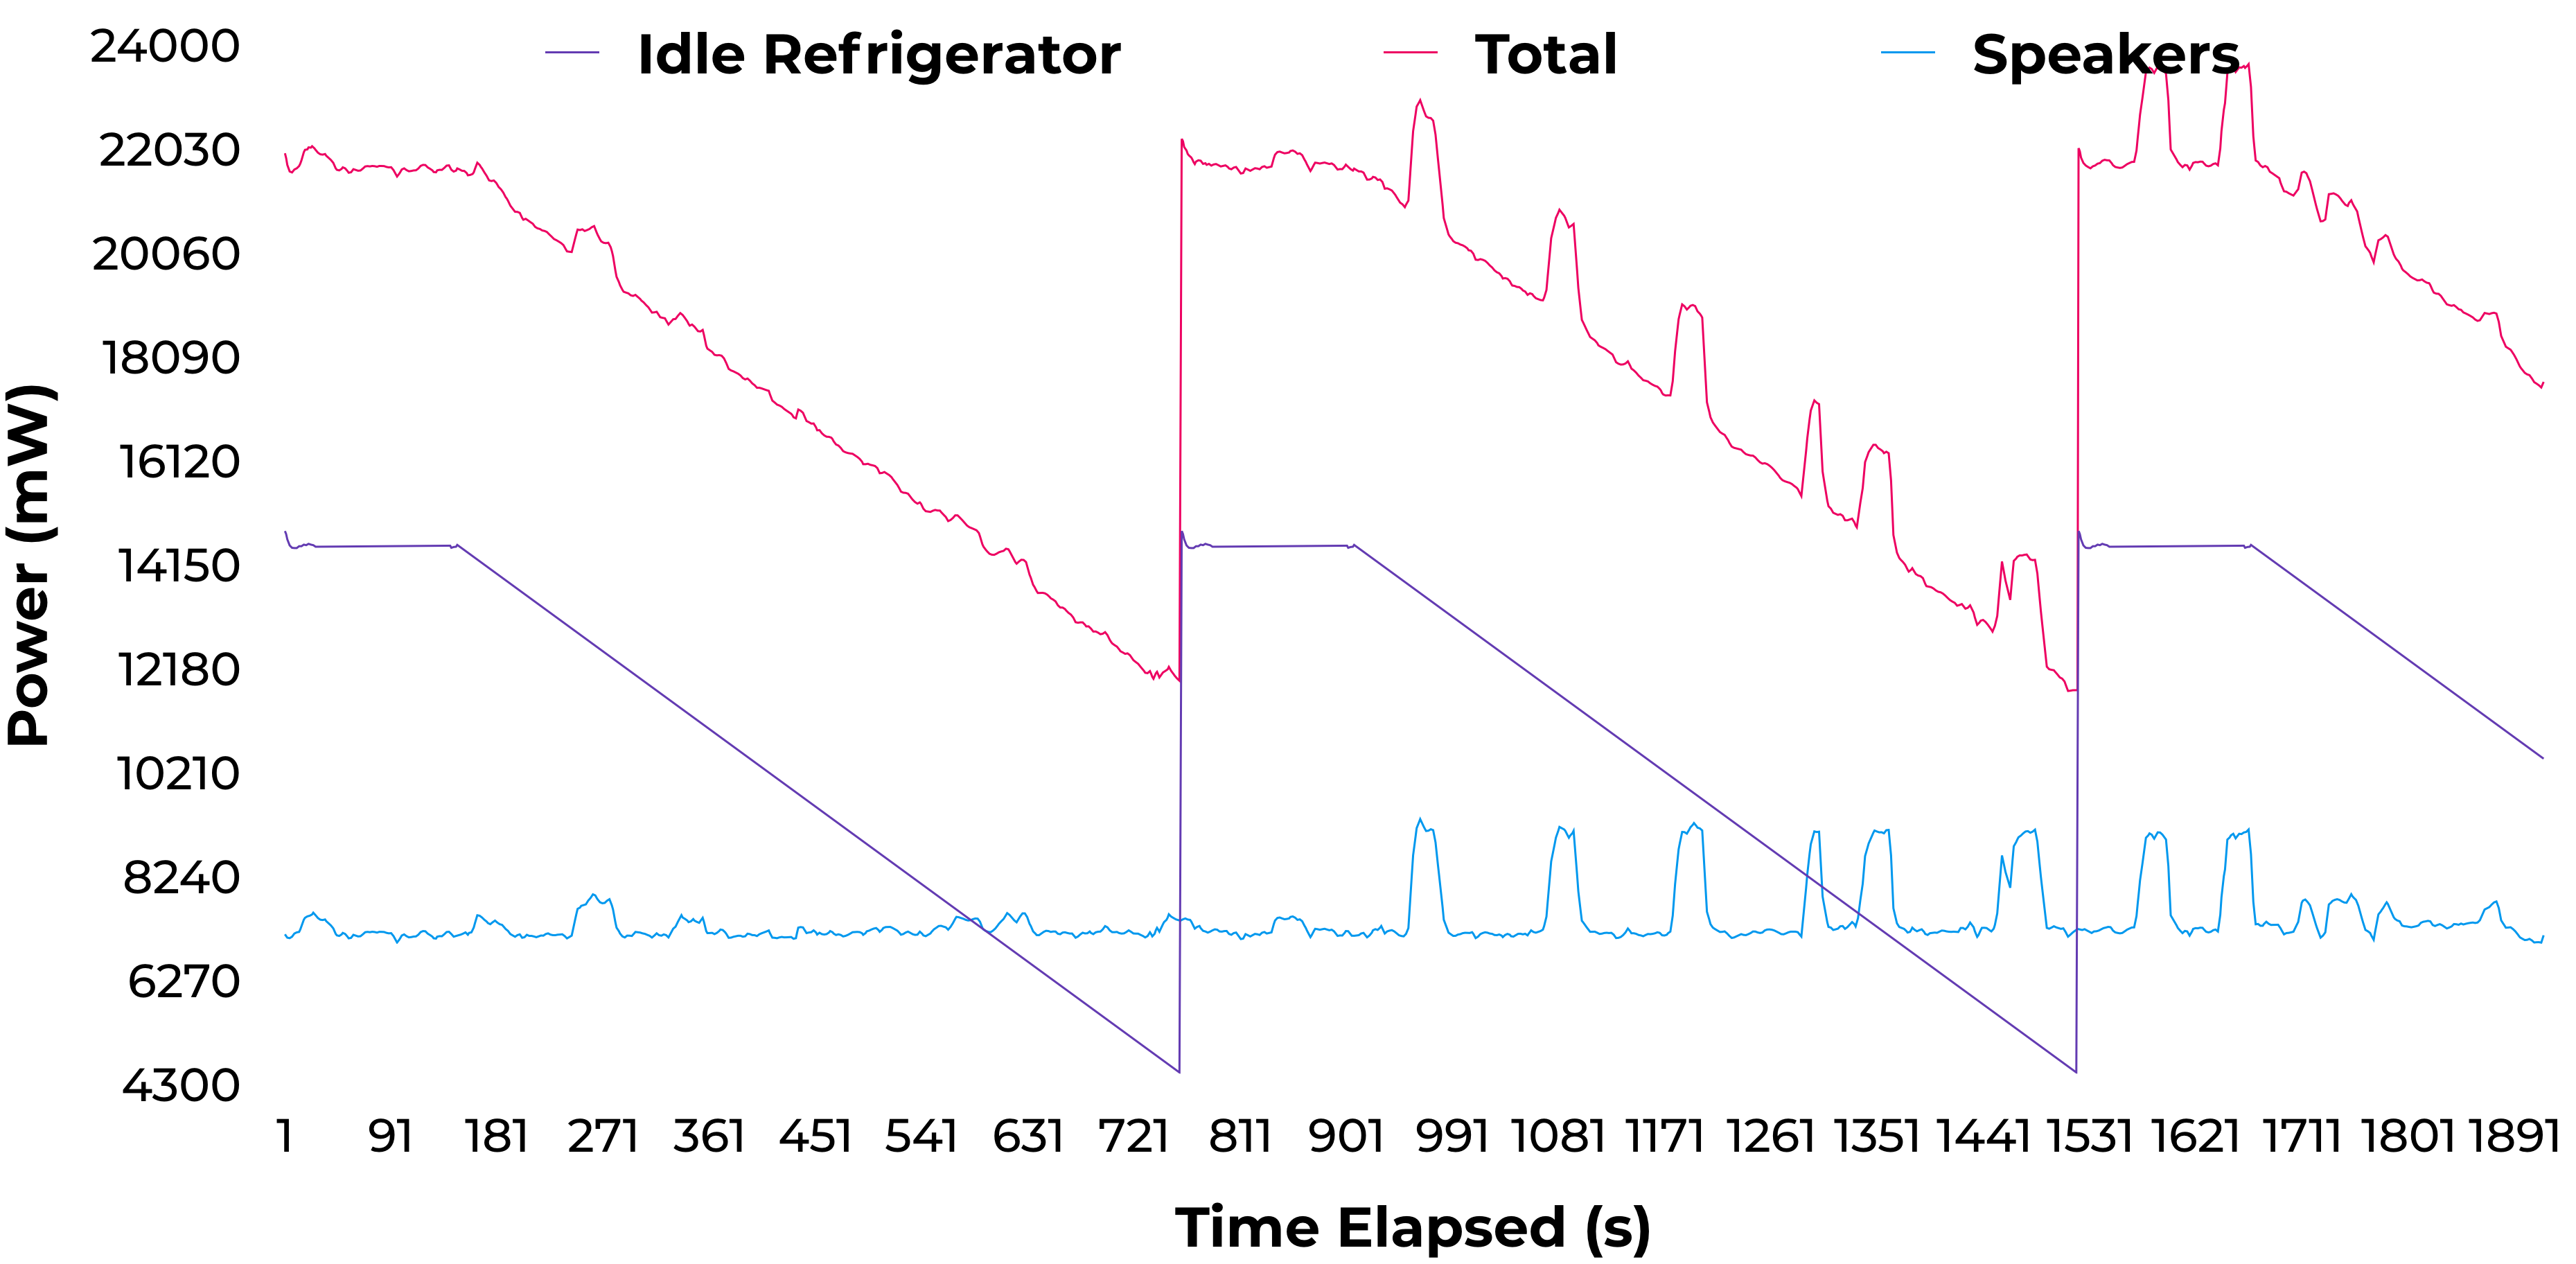
\includegraphics[width=1\textwidth]{figures/idleFridgeNoise.png}
  \caption{Idle refrigerator with figure \ref{fig:bestBballSum} trace.}
  \label{fig:fridgeIdle}
\end{figure}

\begin{figure}[H]
  \centering
  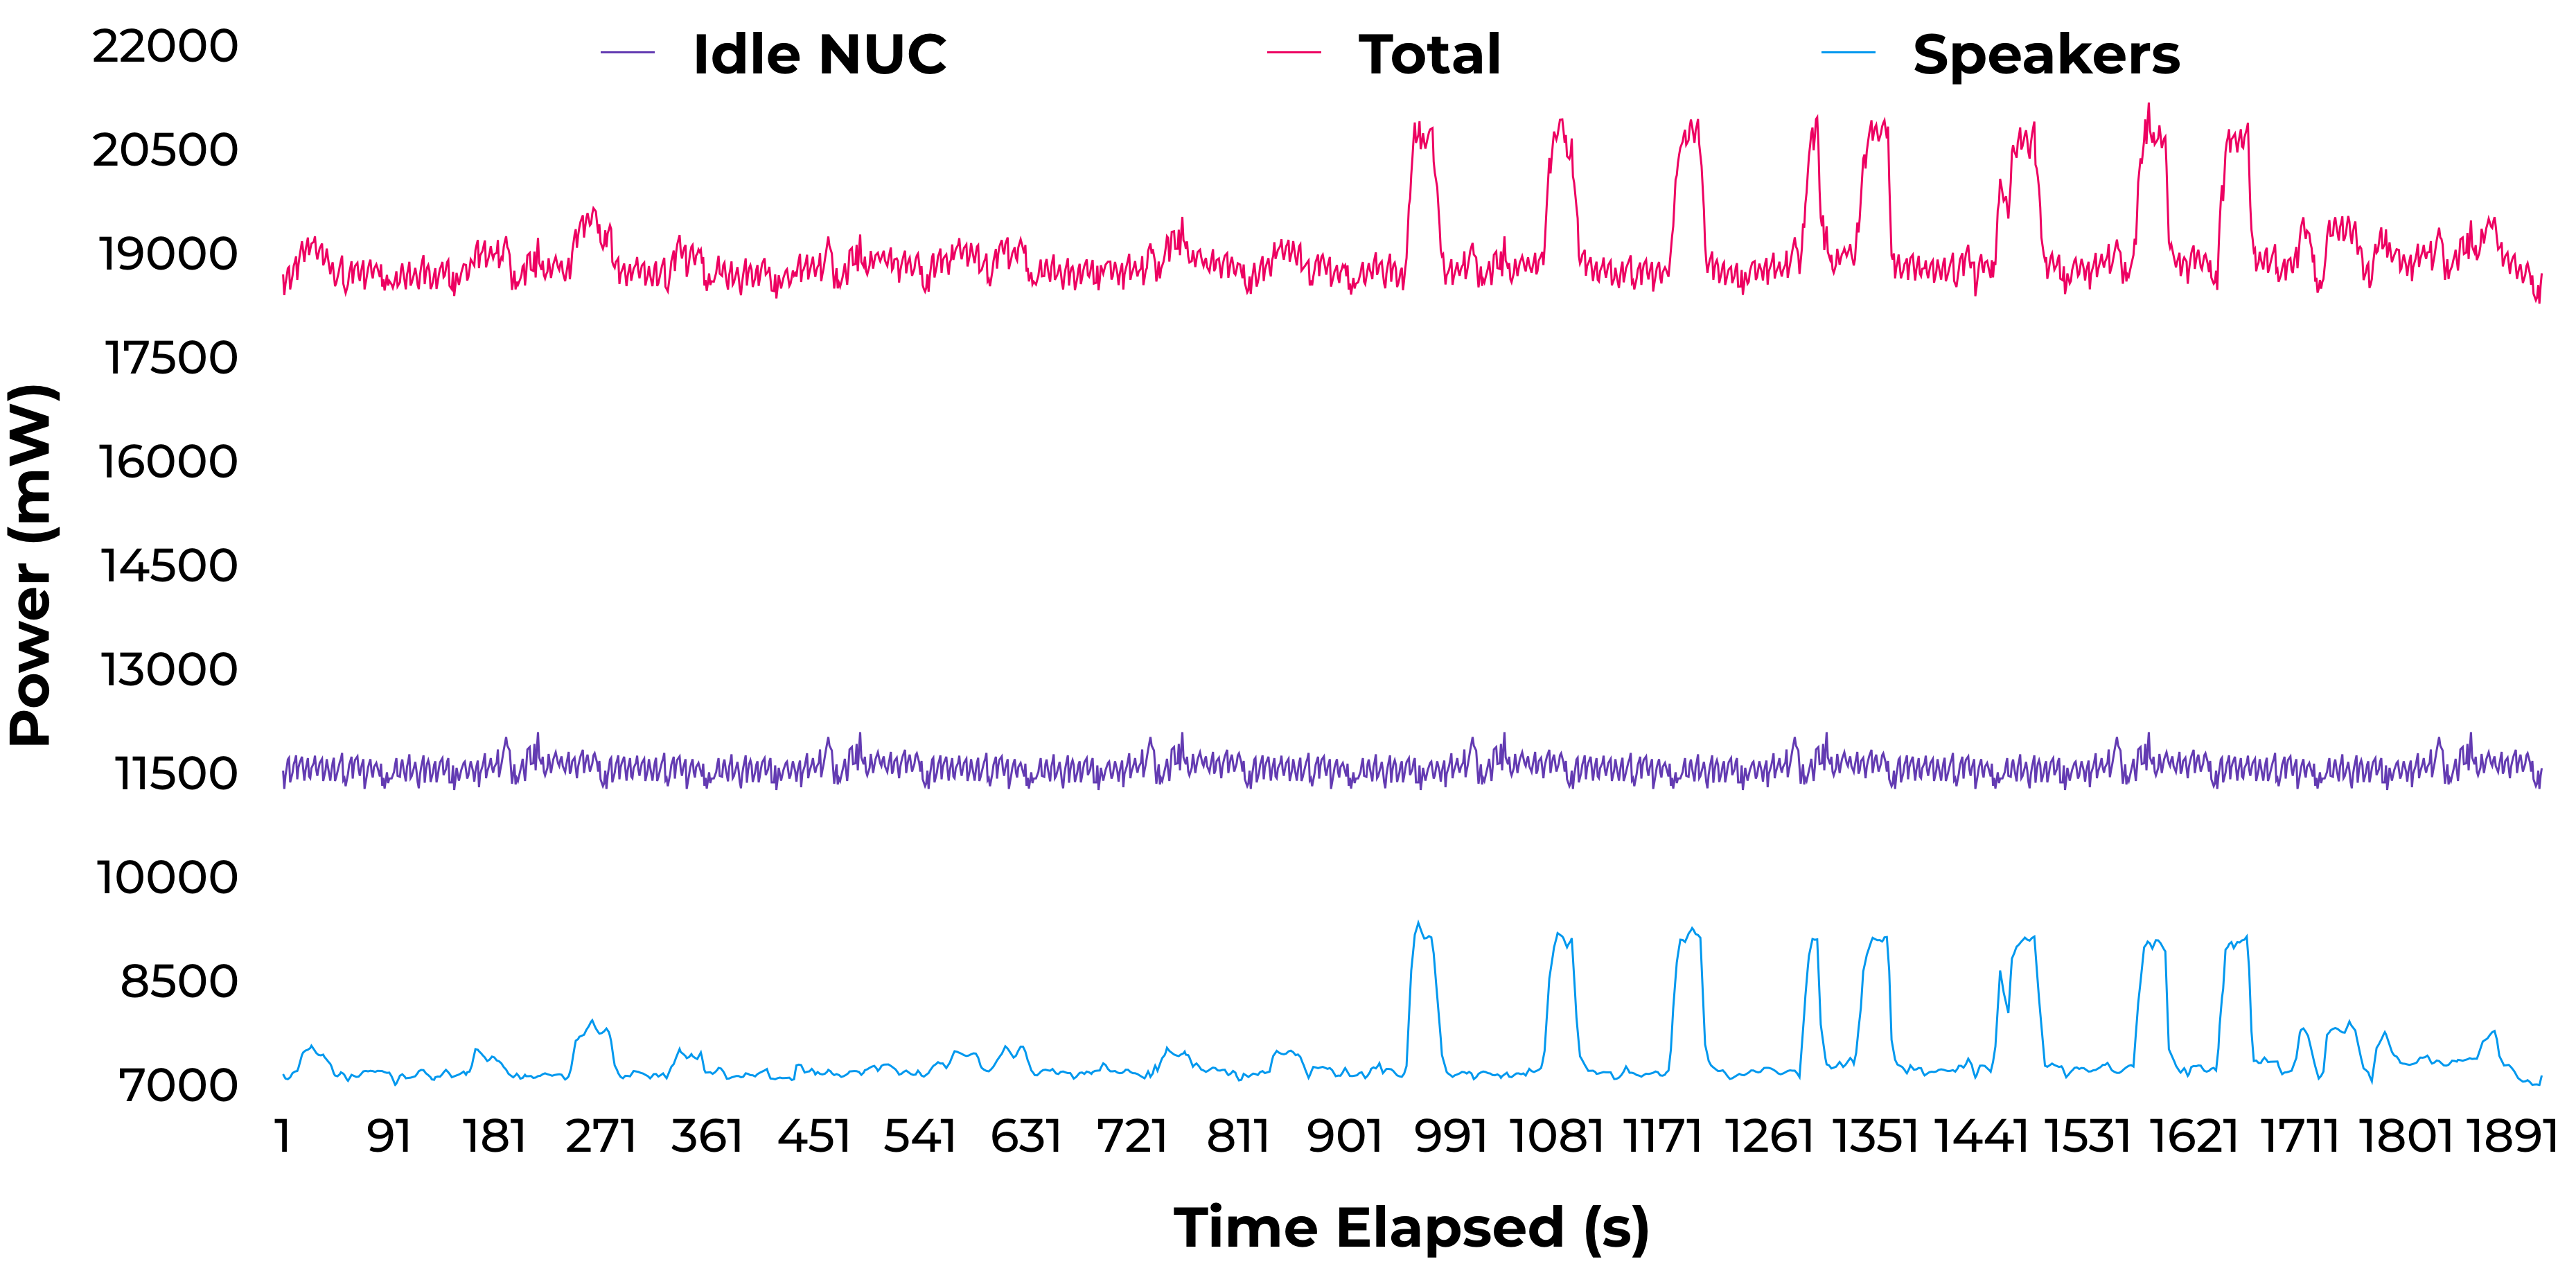
\includegraphics[width=1\textwidth]{figures/idleIntelNUCNoise.png}
  \caption{Idle PC (Intel NUC) with figure \ref{fig:bestBballSum} trace.}
  \label{fig:nucIdle}
\end{figure}

\begin{figure}[H]
    \centering
    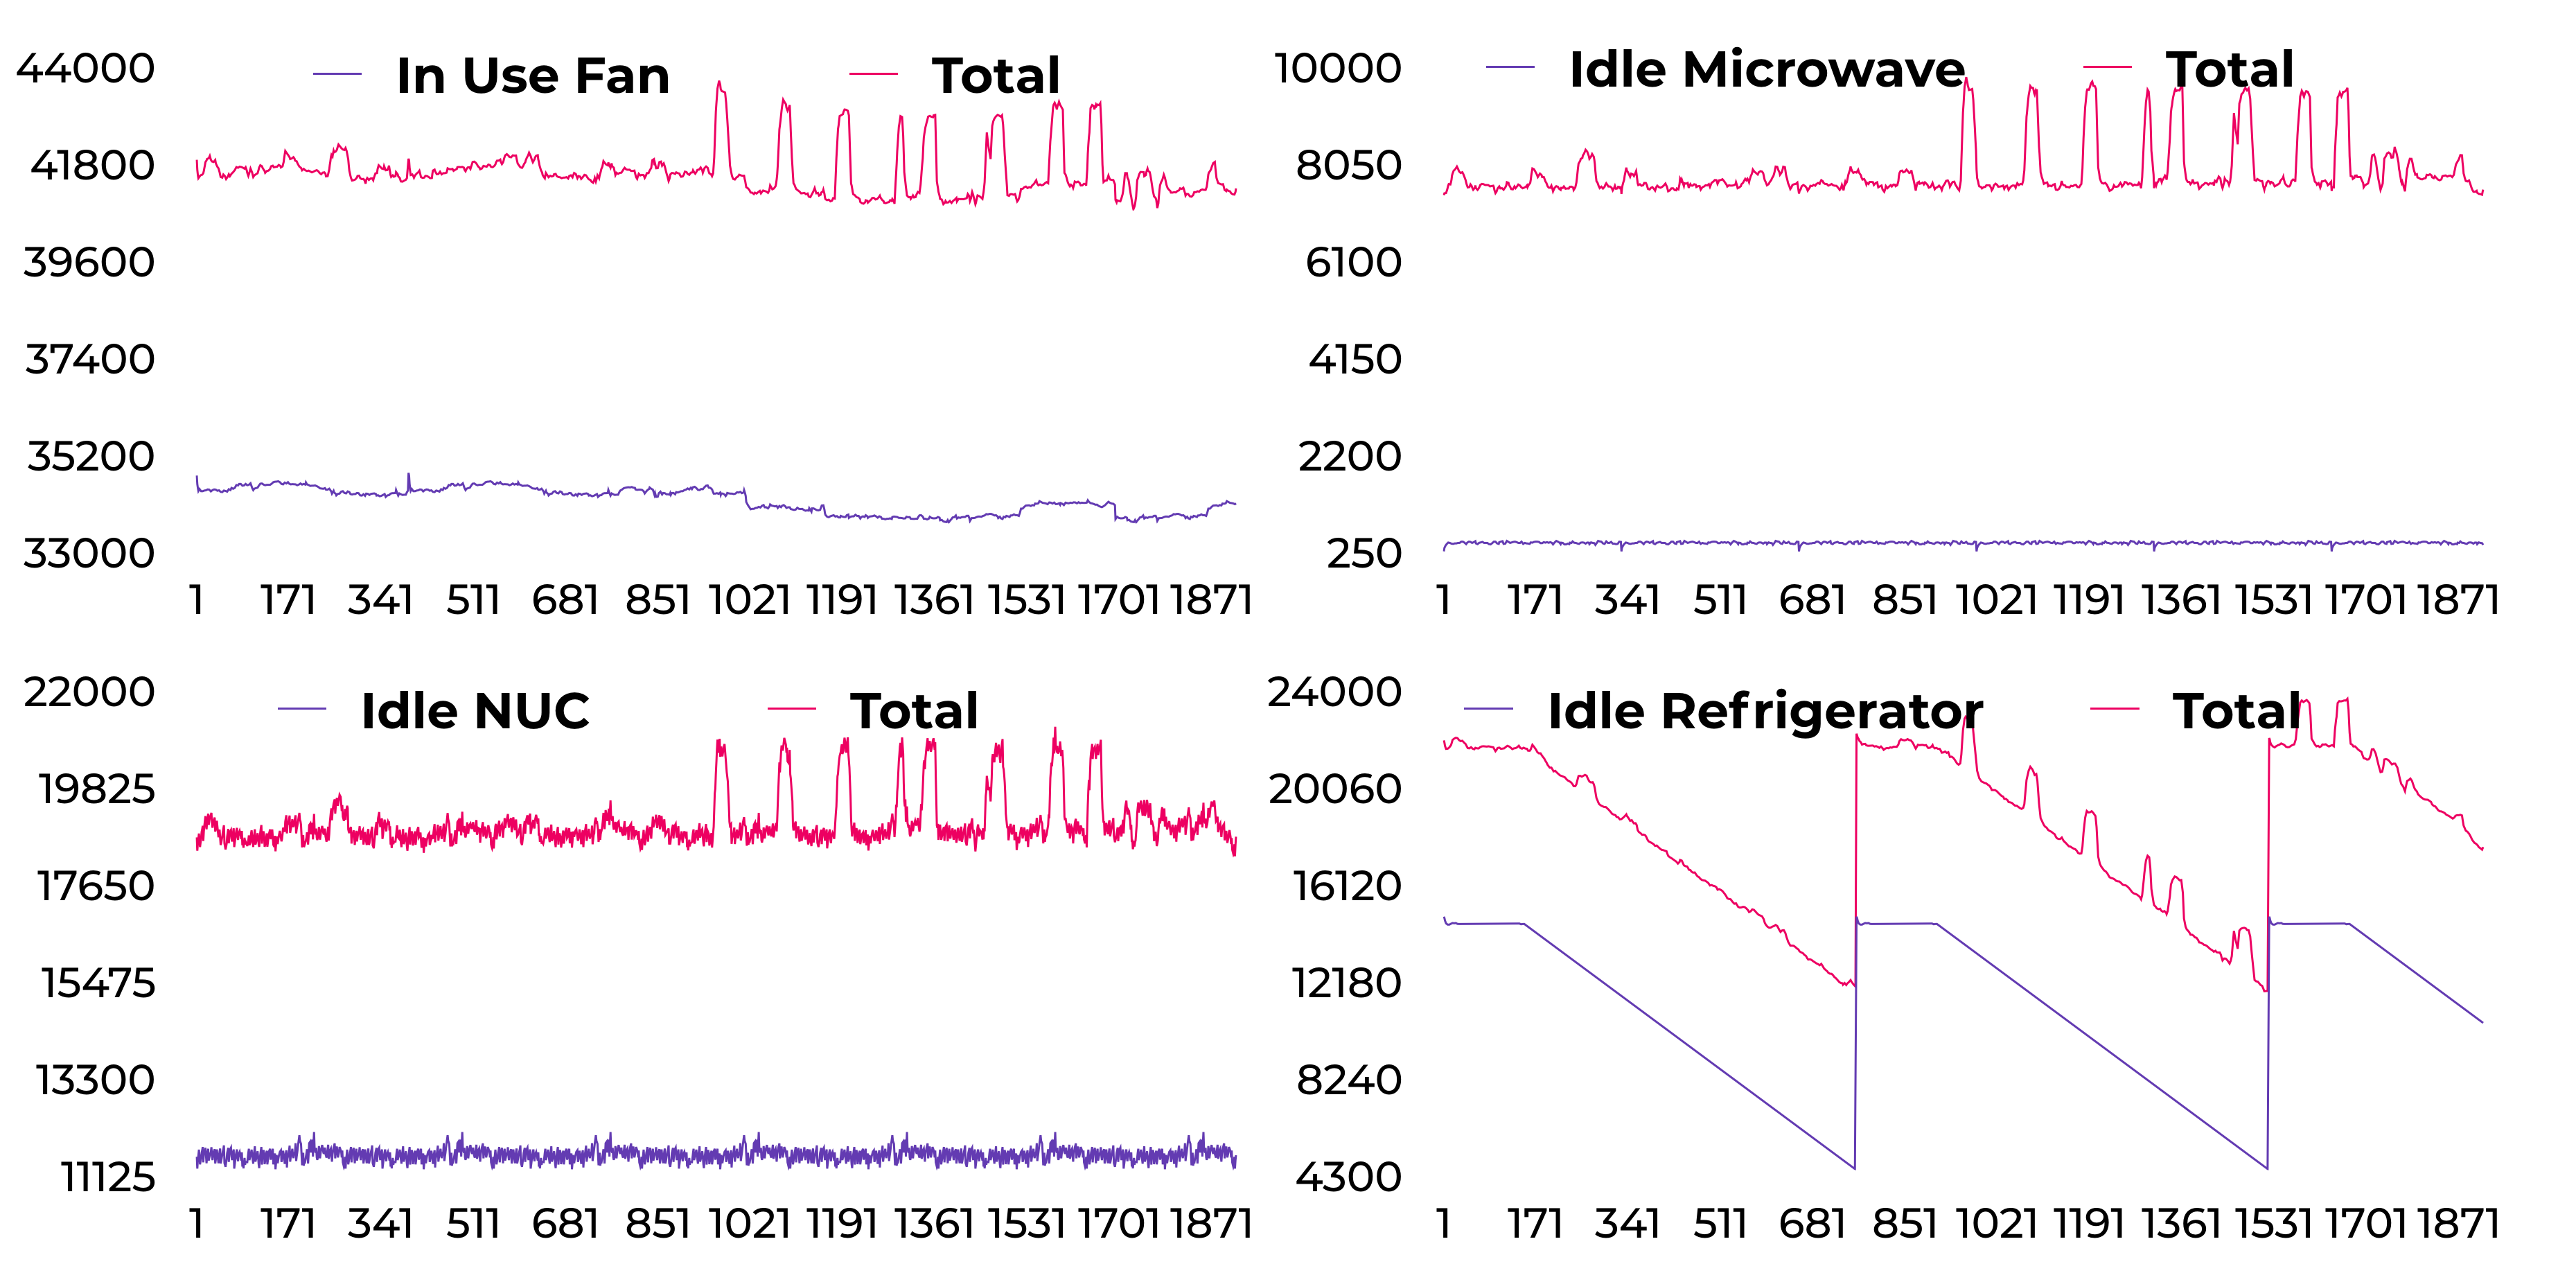
\includegraphics[width=1\textwidth]{figures/allIdleNoise.png}
    \caption{\ref{fig:fanIdle}, \ref{fig:uWaveIdle}, \ref{fig:fridgeIdle}, and \ref{fig:nucIdle} figures zoomed in}
    \label{fig:allIdleNoise}
  \end{figure}

\begin{figure}[H]
  \centering
  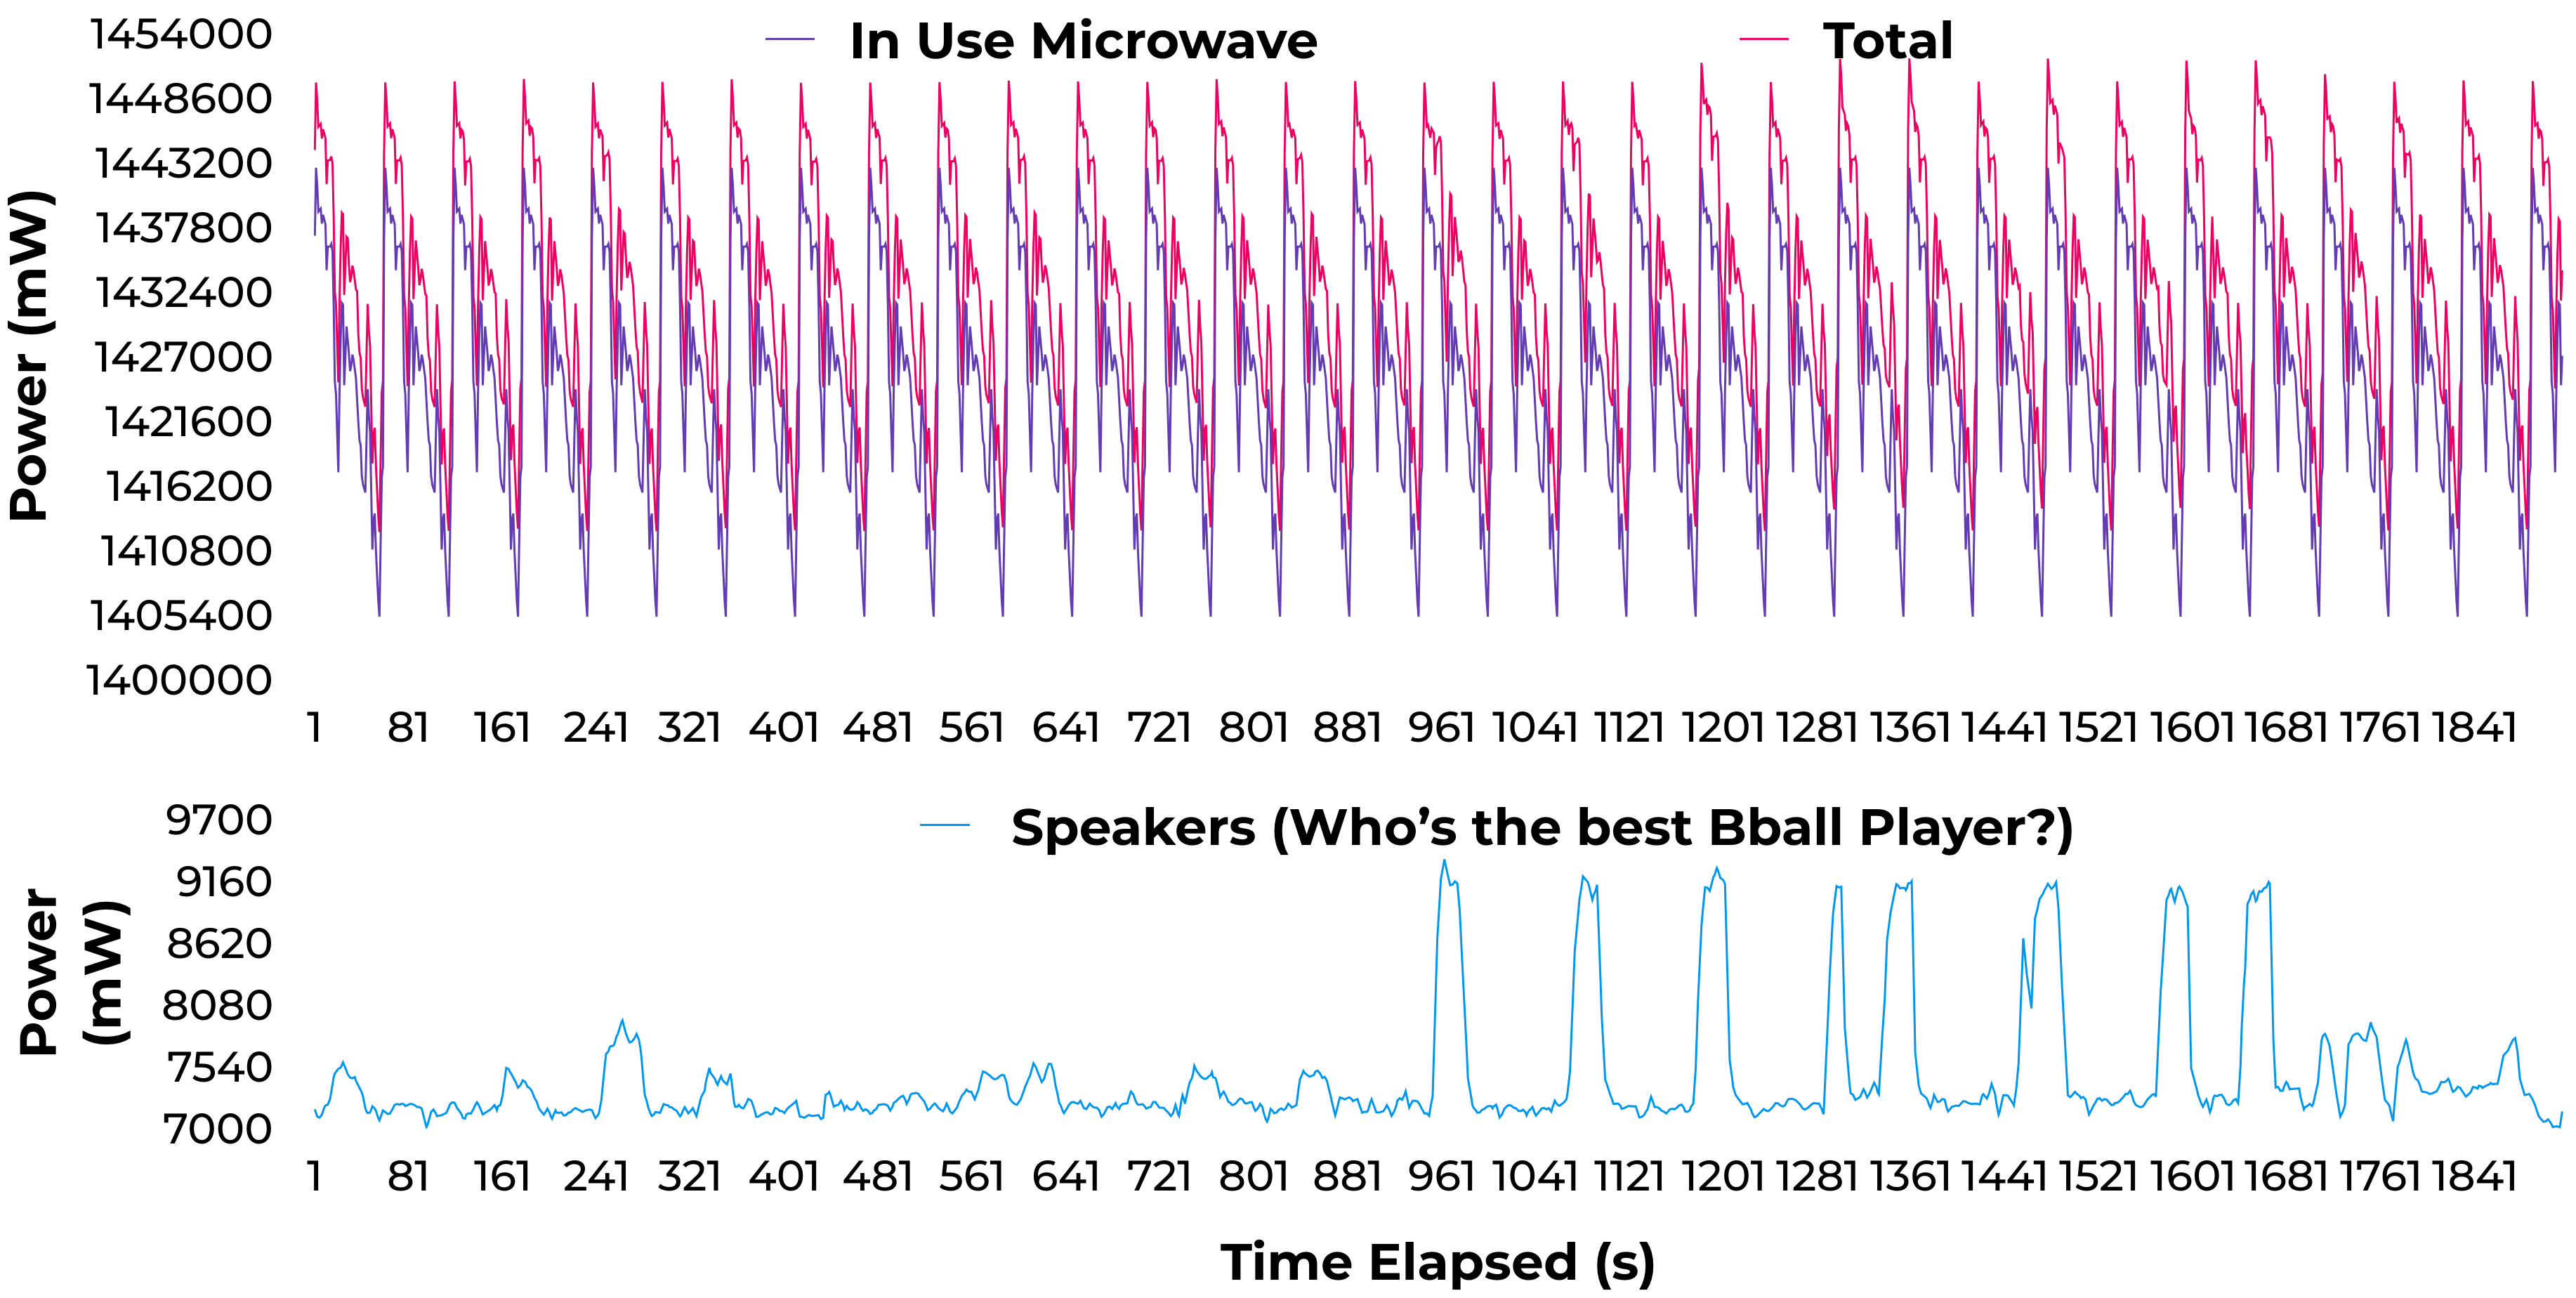
\includegraphics[width=1\textwidth]{figures/inUseuWaveNoiseSeperate.png}
  \caption{In use Microwave with figure \ref{fig:bestBballSum} trace seperately.}
  \label{fig:uWaveInUseSeperate}
\end{figure}

\begin{figure}[H]
  \centering
  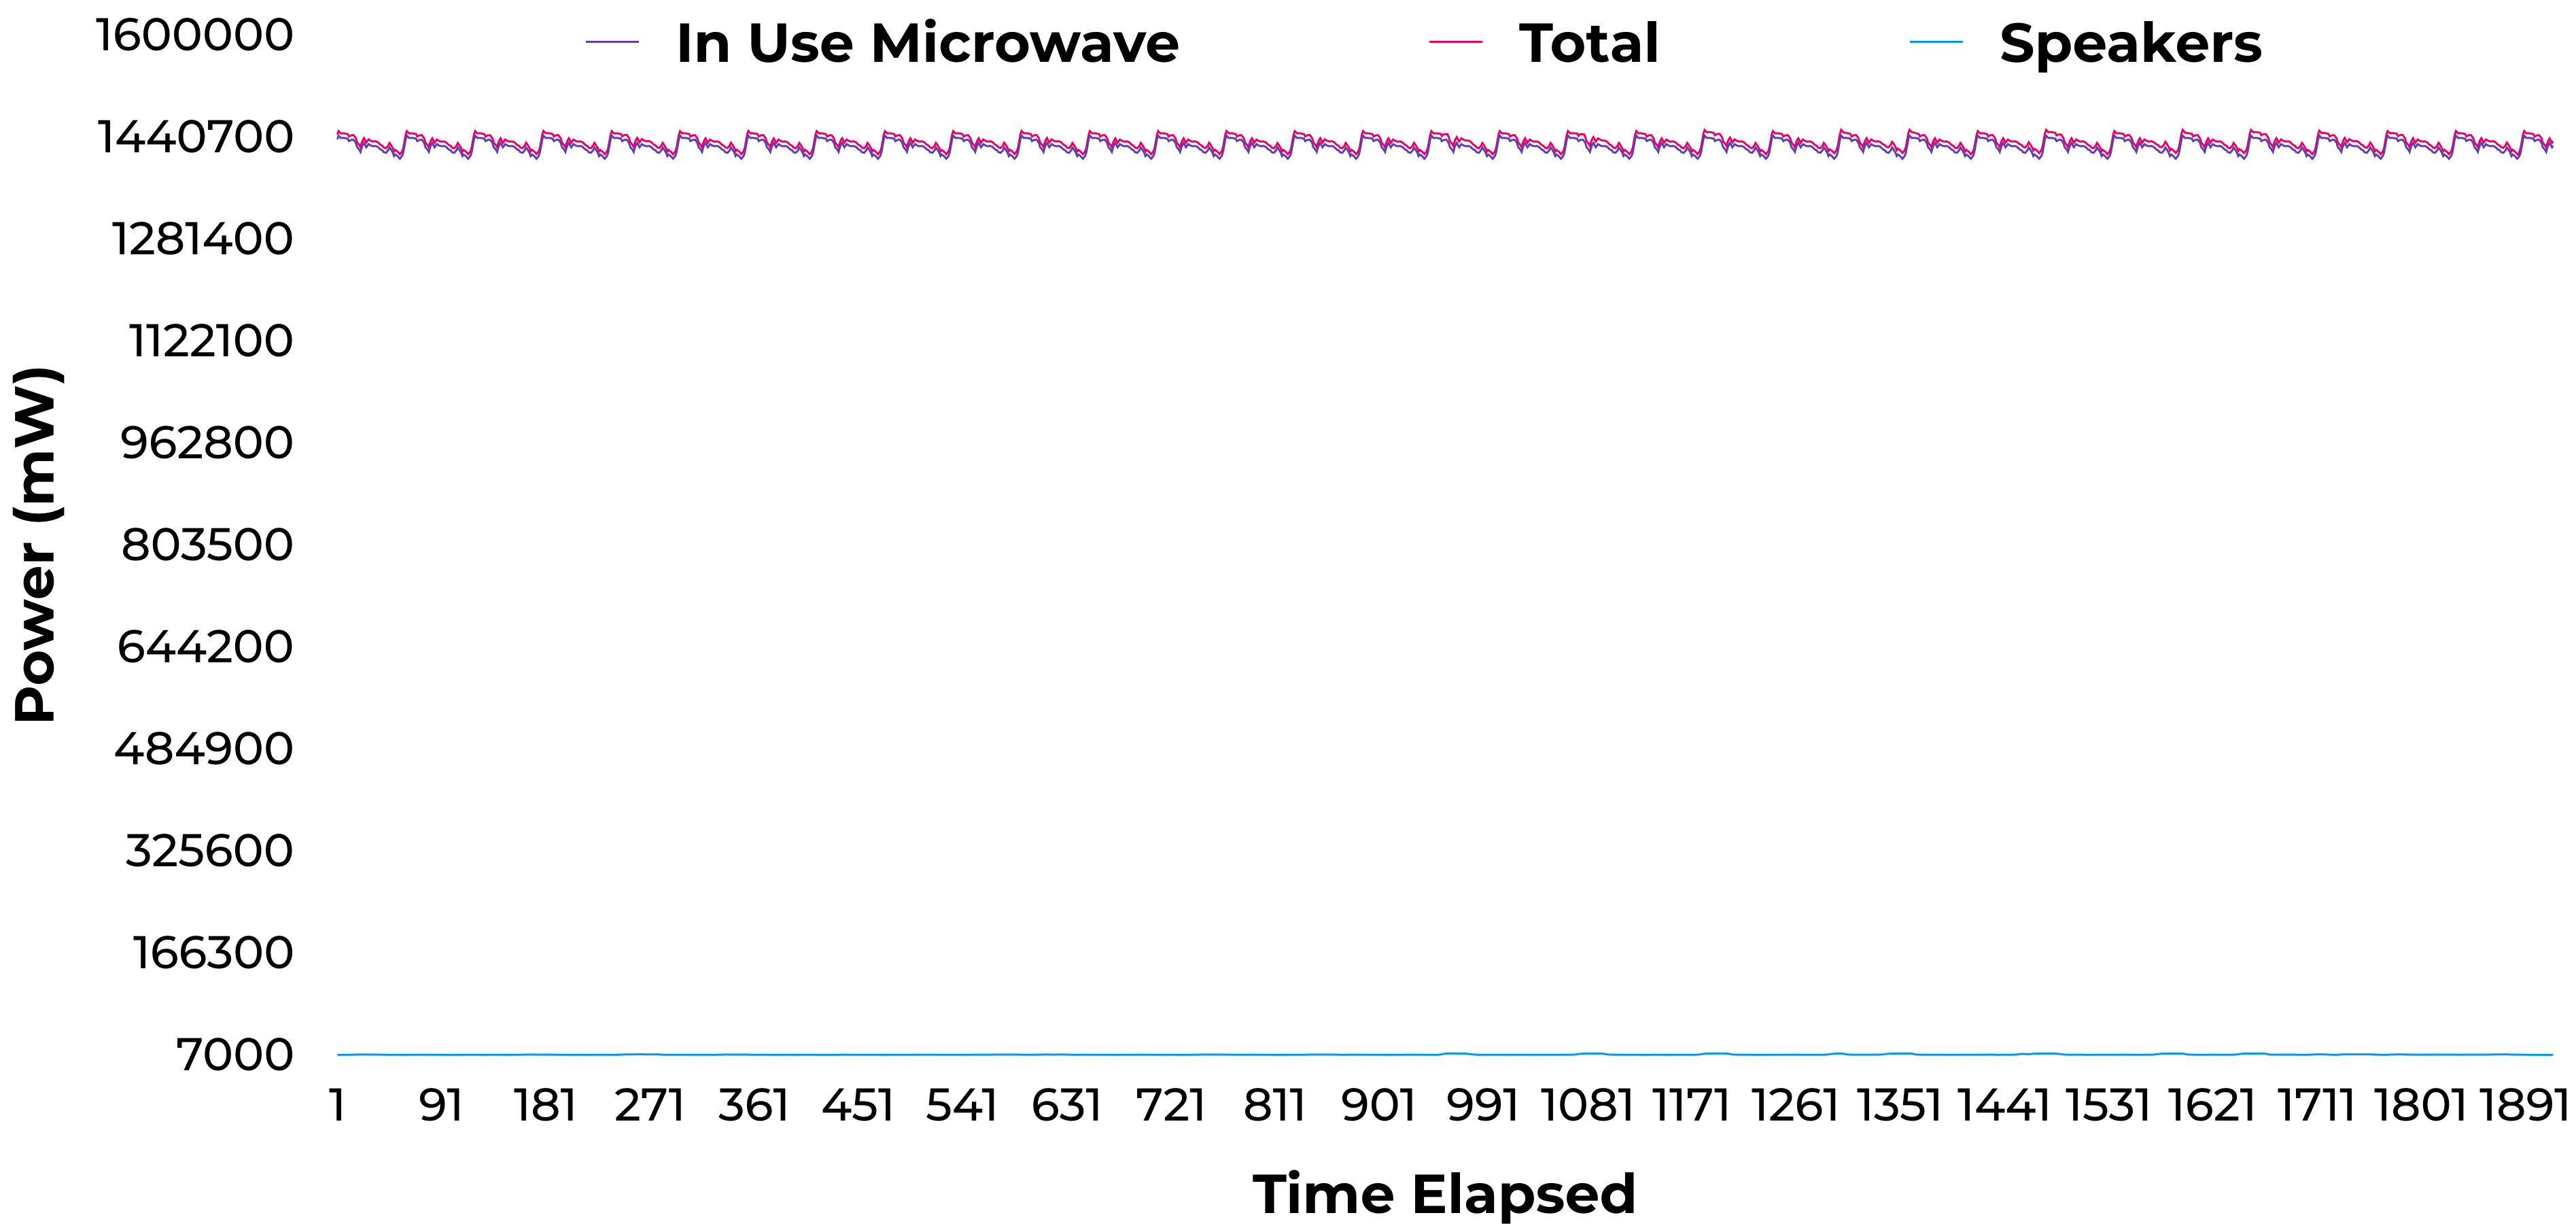
\includegraphics[width=1\textwidth]{figures/inUseuWaveNoise.png}
  \caption{In use Microwave with figure \ref{fig:bestBballSum} trace.}
  \label{fig:uWaveInUse}
\end{figure}

\begin{figure}[H]
  \centering
  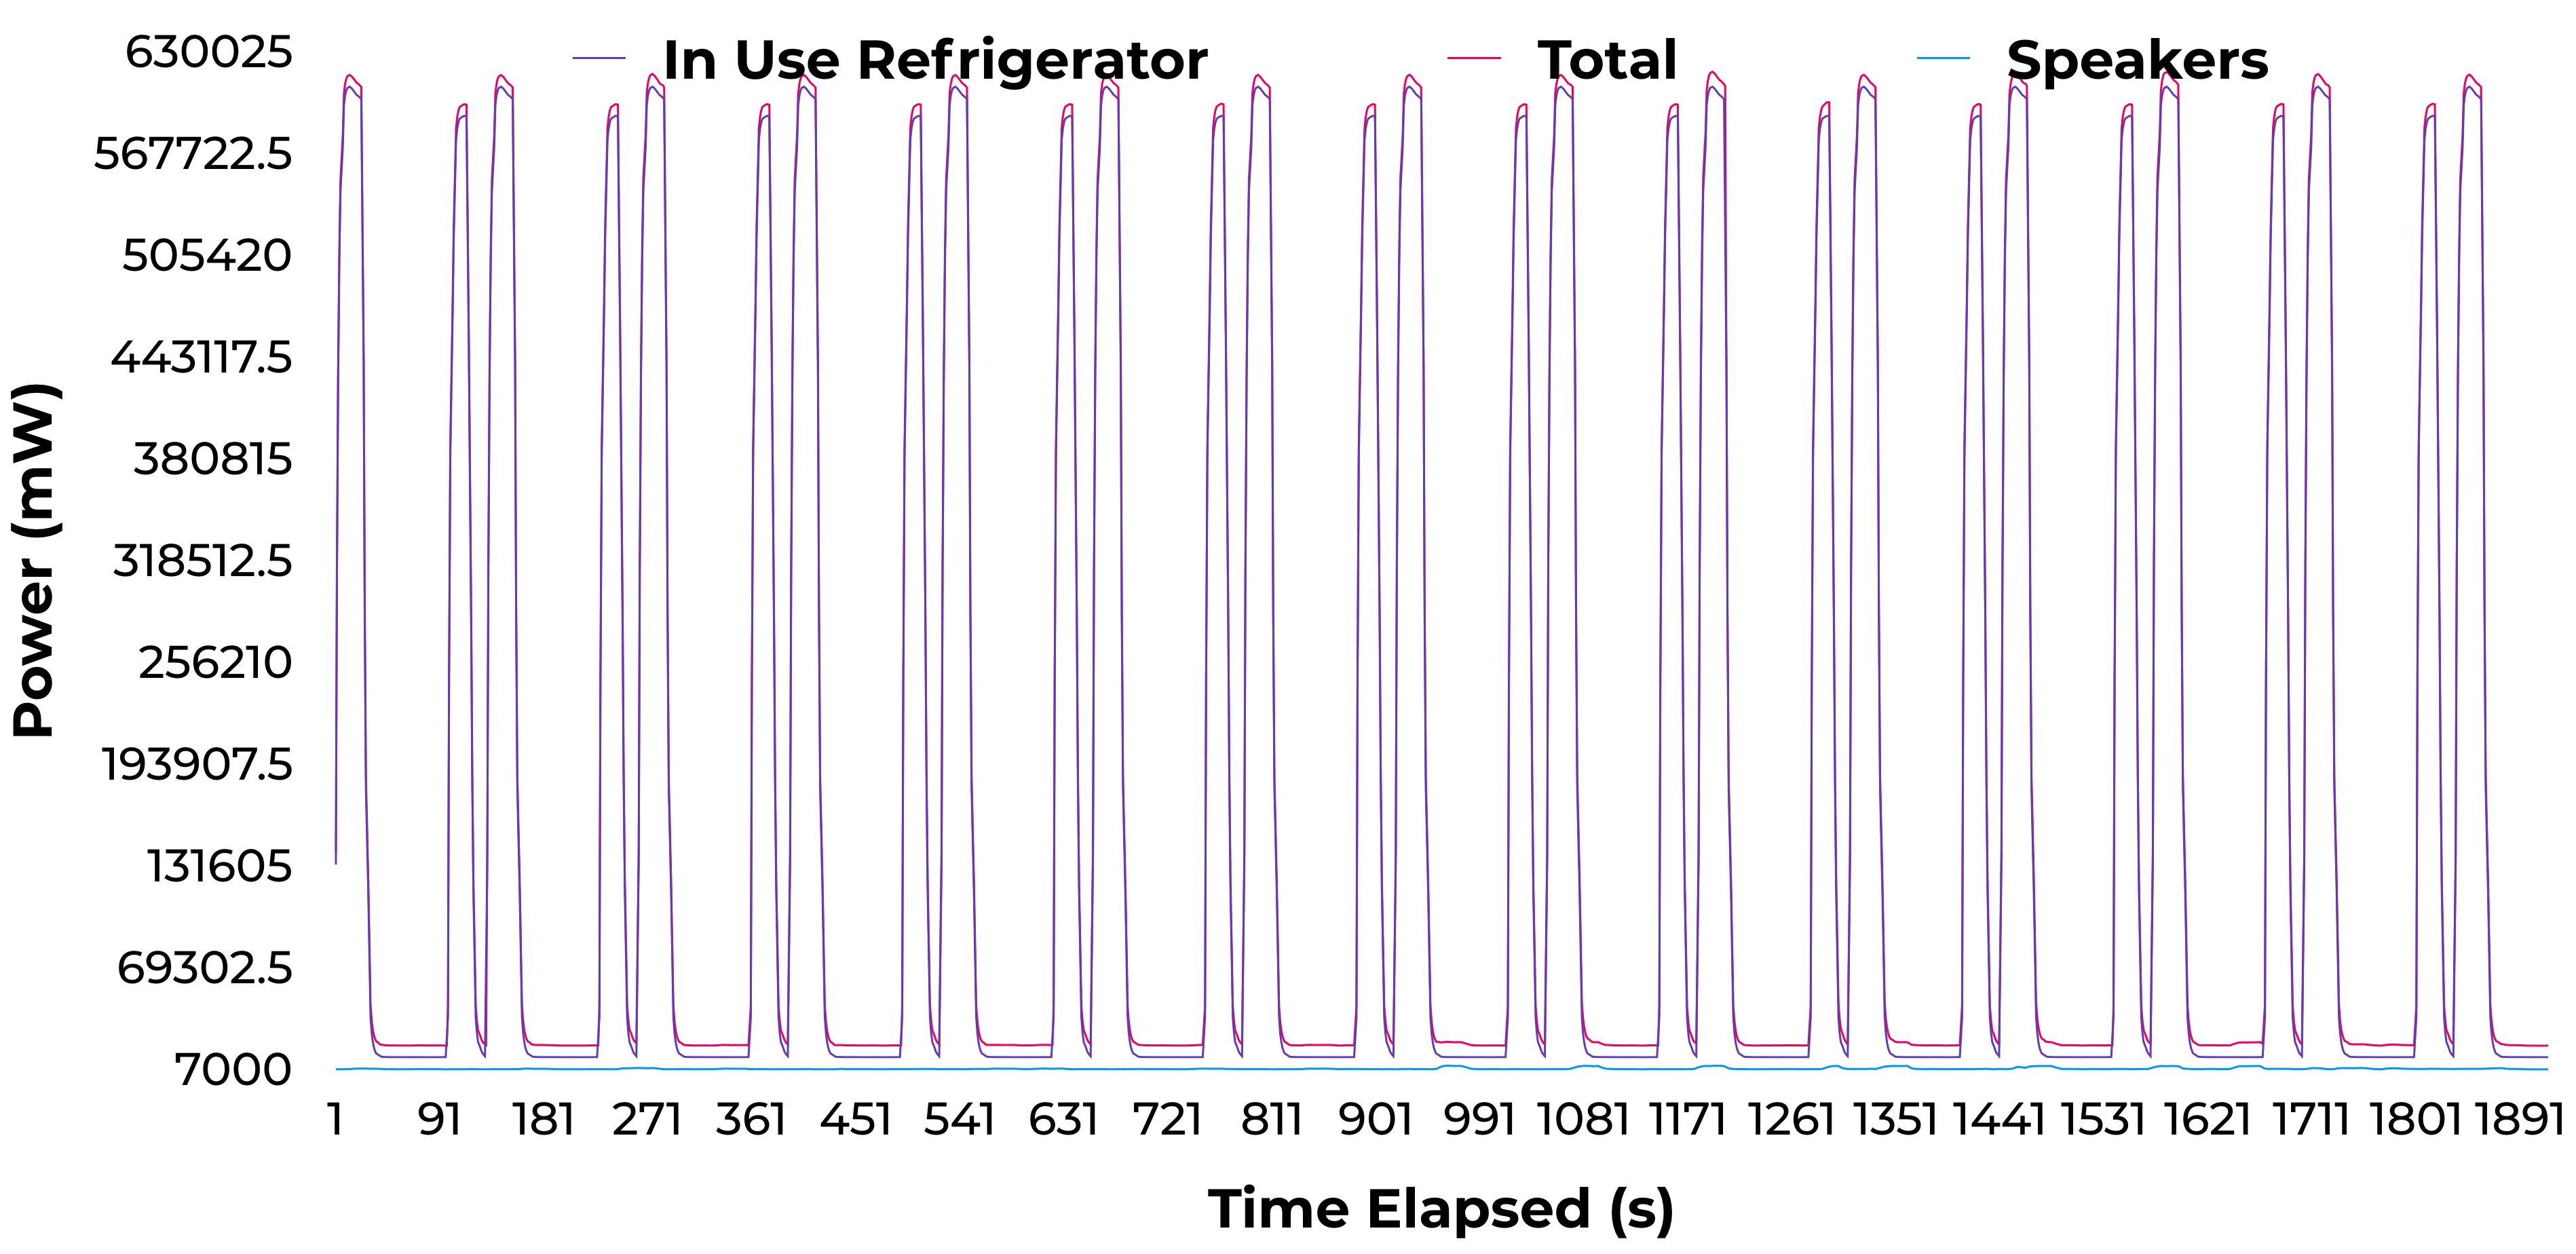
\includegraphics[width=1\textwidth]{figures/inUseFridgeNoise.png}
  \caption{Fridge in the middle of cooling with figure \ref{fig:bestBballSum} trace.}
  \label{fig:fridgeInUse}
\end{figure}

\begin{figure}[H]
  \centering
  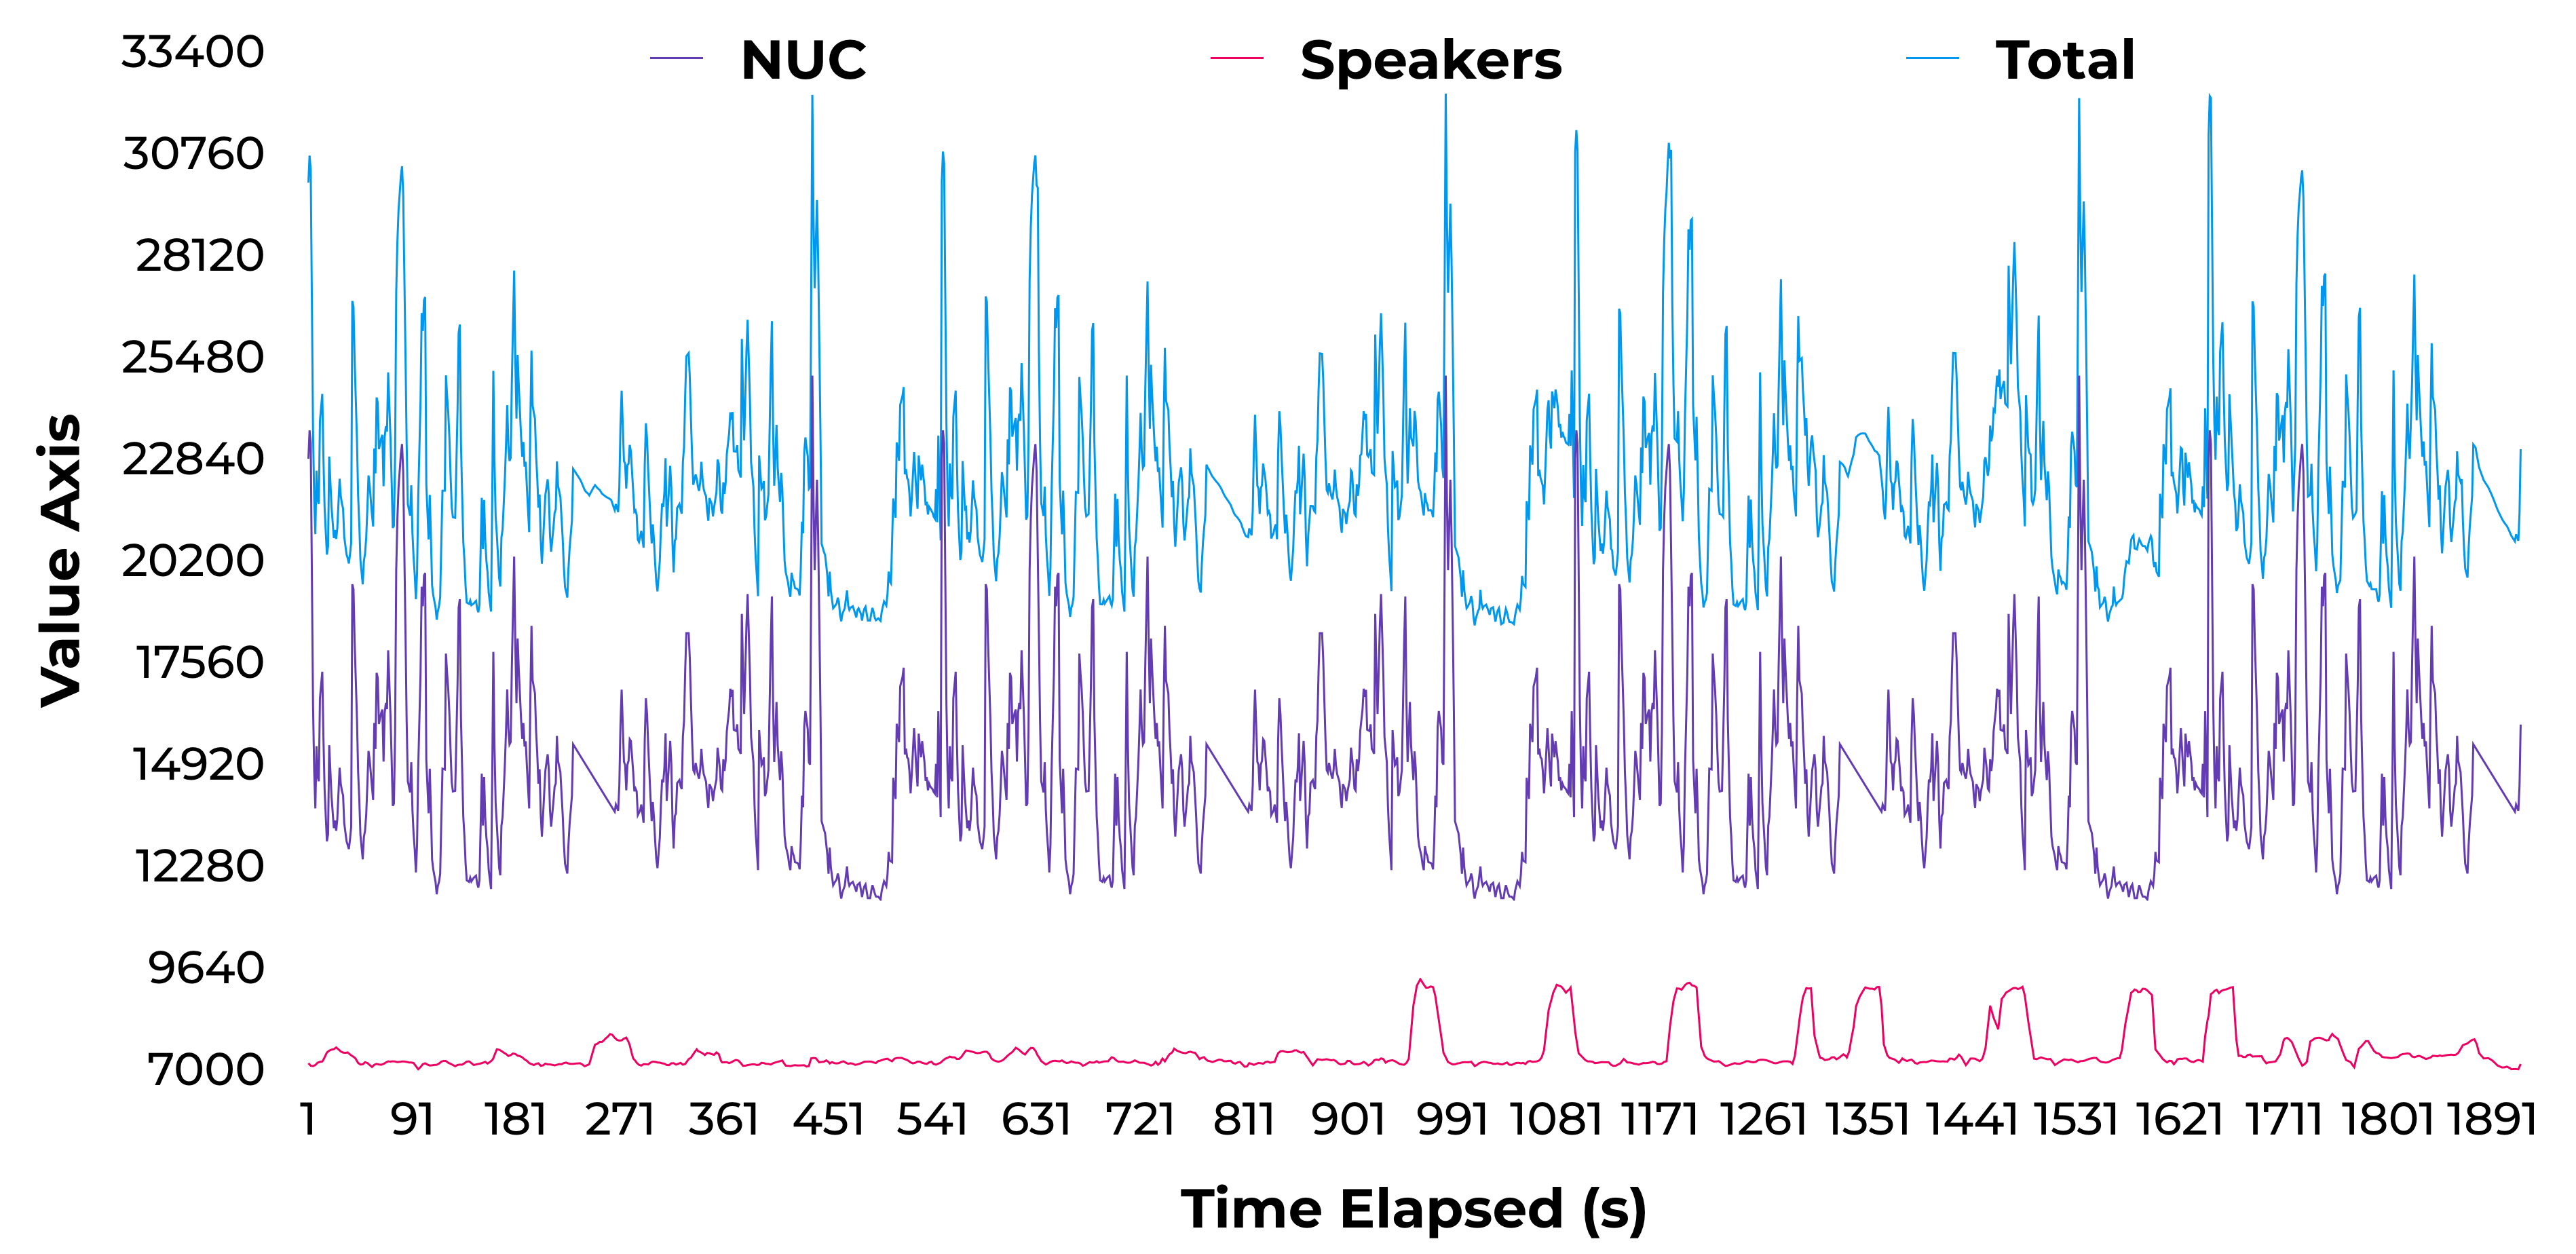
\includegraphics[width=1\textwidth]{figures/inUseNUCNoise.png}
  \caption{PC in use with figure \ref{fig:bestBballSum} trace.}
  \label{fig:nucInUse}
\end{figure}

The figures above show that it is possible to determine the smart speaker in use from visual examination of power spikes even in the presence of noise. If the noise within the house is stable, the power spikes will just be shifted up as shown in figure \ref{fig:fanIdle}. If the noise within the house is low power then, the spikes will visually overpower the noise, as shown in figure \ref{fig:nucIdle}.

But if the noise within the house is large in magnitude such as the microwave or fridge while in use \ref{fig:uWaveInUse} \ref{fig:fridgeInUse}, then the large power usage by these decices will completely squash the power spikes from the smart speakers. The spikes can no longer be seen, even when zoomed in, as shown in figure \ref{fig:uWaveInUseSeperate}. The smart speaker spikes also dissapear if the noise of a device is on the same or a larger magnitude than the power spikes, as shown in figure \ref{fig:nucInUse}. The power spikes can still be seen in the sum graph for this figure, but it would be impossible to visually differentiate between a power spike from a speaker and from the noise without knowing the original smart speaker graph.

These two cases occur depending on the house. If a lot of battery power devices such as laptops or phones are used in a house then it would would still be possible to visually determine the power spikes. Or in another case, if high power devices such as the microwave or fridge are not in use often, then the smart speaker spikes can be visually correlated. But if a household has a lot of devices plugged into an outlet for power, then the smart speaker power spikes will dissapear in the cumalative nosie of all the devices. In the first case, there are privacy implications in what could be learned from a household's power line information, which are easily accessible in most households today \cite{griffith_2017}.

\section{Smart Speaker Comparison}
\label{smartSpeakerComparisonSection}
The figures in section \ref{sumPowerGraph} show that the Echo Dot uses a lot more energy than the other smart speakers. Because of this, we wanted to compare the energy and network usages of the three smart speakers individually so that we can determine trade-offs that they make.

In the figures \ref{fig:smartSpeakerSeperate} and \ref{fig:smartSpeakerNetworkSeperate}, we display power and network traces for the Echo Dot 1, Eufy Genie 1, and Google Home. We used the same time frame as the graph in figure \ref{fig:bestBballSeperate} for the two graphs below. We removed the second Echo Dot and Eufy Genie for simplicity.

In the same time frame as the two graphs below, we also recorded the average power usage and throughput for the smart speakers. For average power, from greatest to least, we have the Echo Dot (1650 mW), Eufy Genie (1325 mW), Google Home (1175 mW). For average throughput, from greatest to least, we have the Eufy Genie (1743 bytes), Google Home (800 bytes), Echo Dot (325 bytes).

\begin{figure}[H]
  \centering
  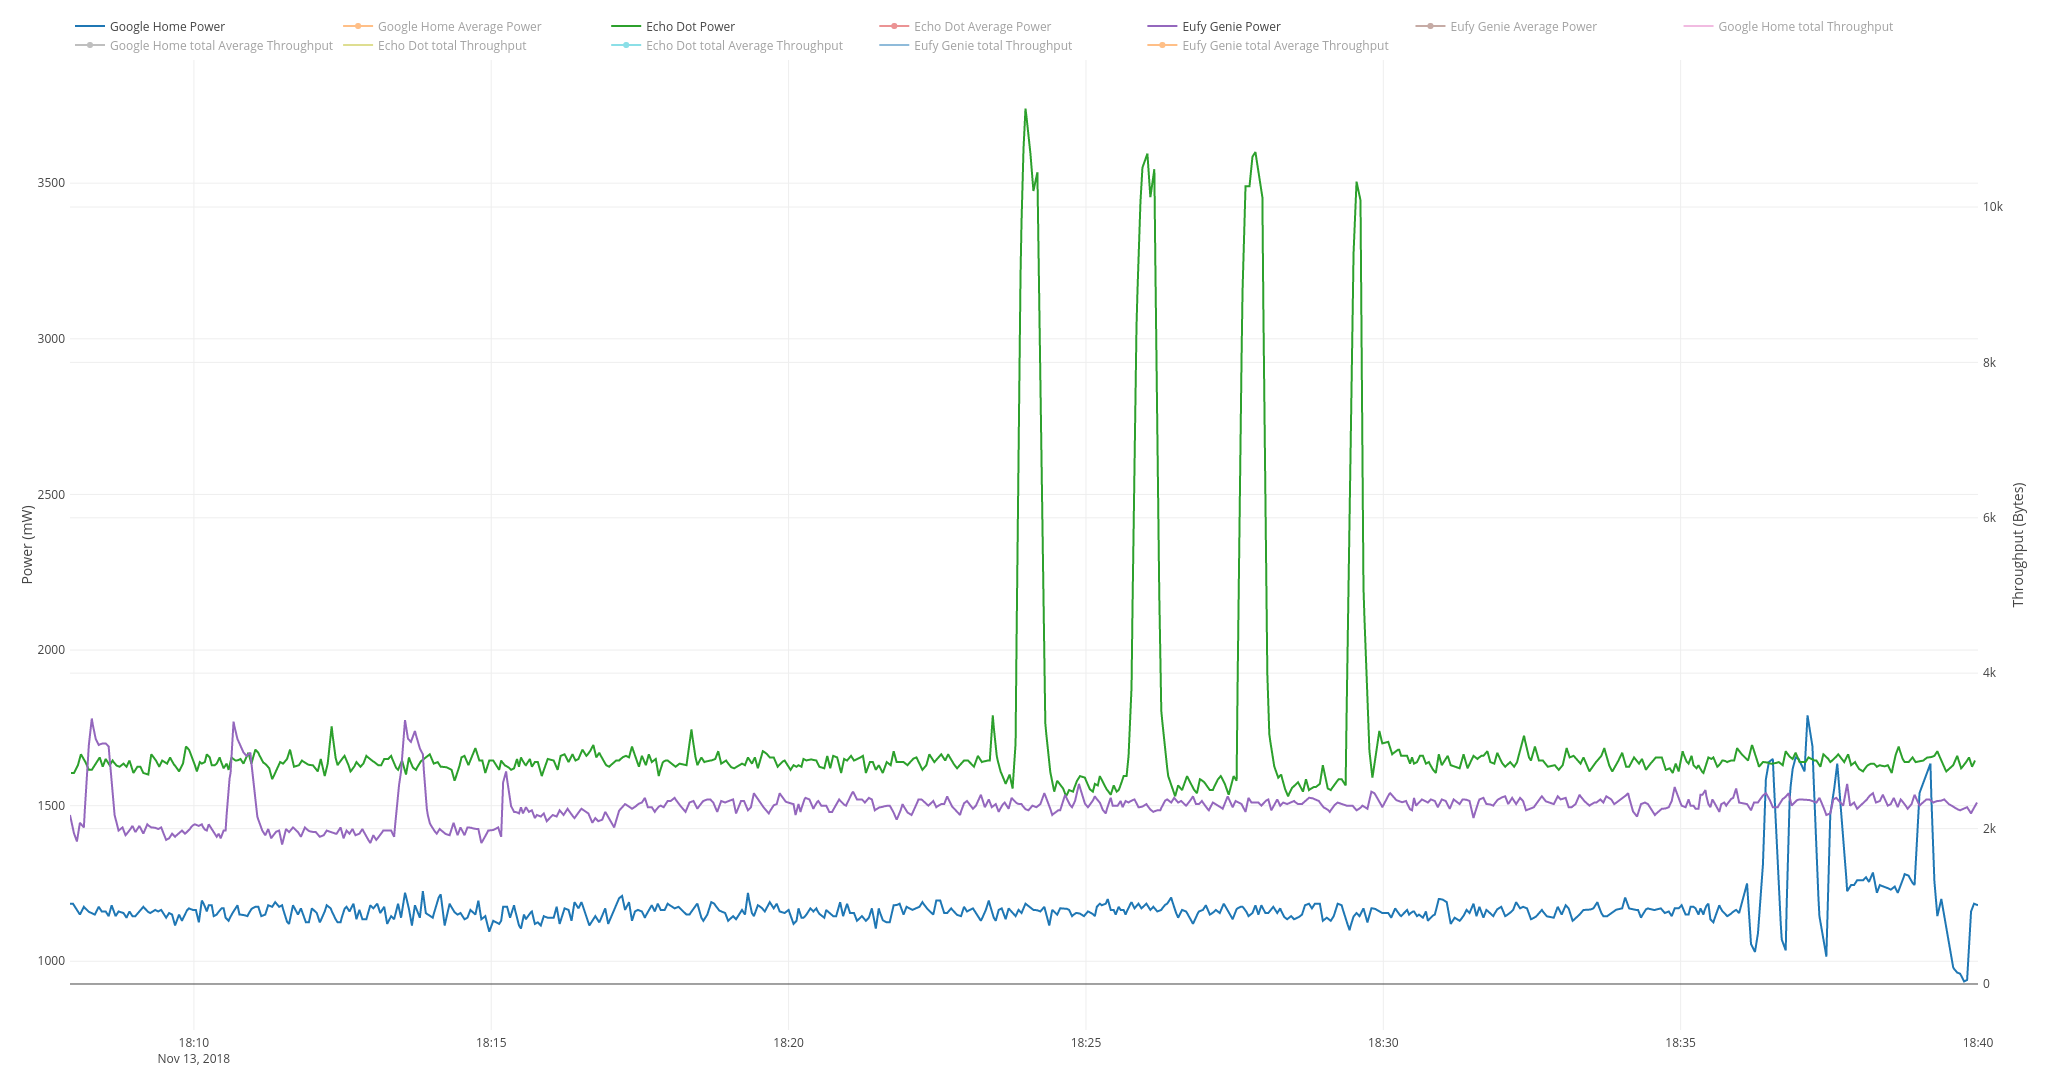
\includegraphics[width=1\textwidth]{figures/smartSpeakerSeperate.png}
  \caption{Power usage of Echo Dot 1, Eufy Genie 1, and Google Home over time when asked ``who is the best basketball player''. Same graph as figure \ref{fig:bestBballSeperate} with Echo Dot 2 and Eufy Genie removed.}
  \label{fig:smartSpeakerSeperate}
\end{figure}

\begin{figure}[H]
  \centering
  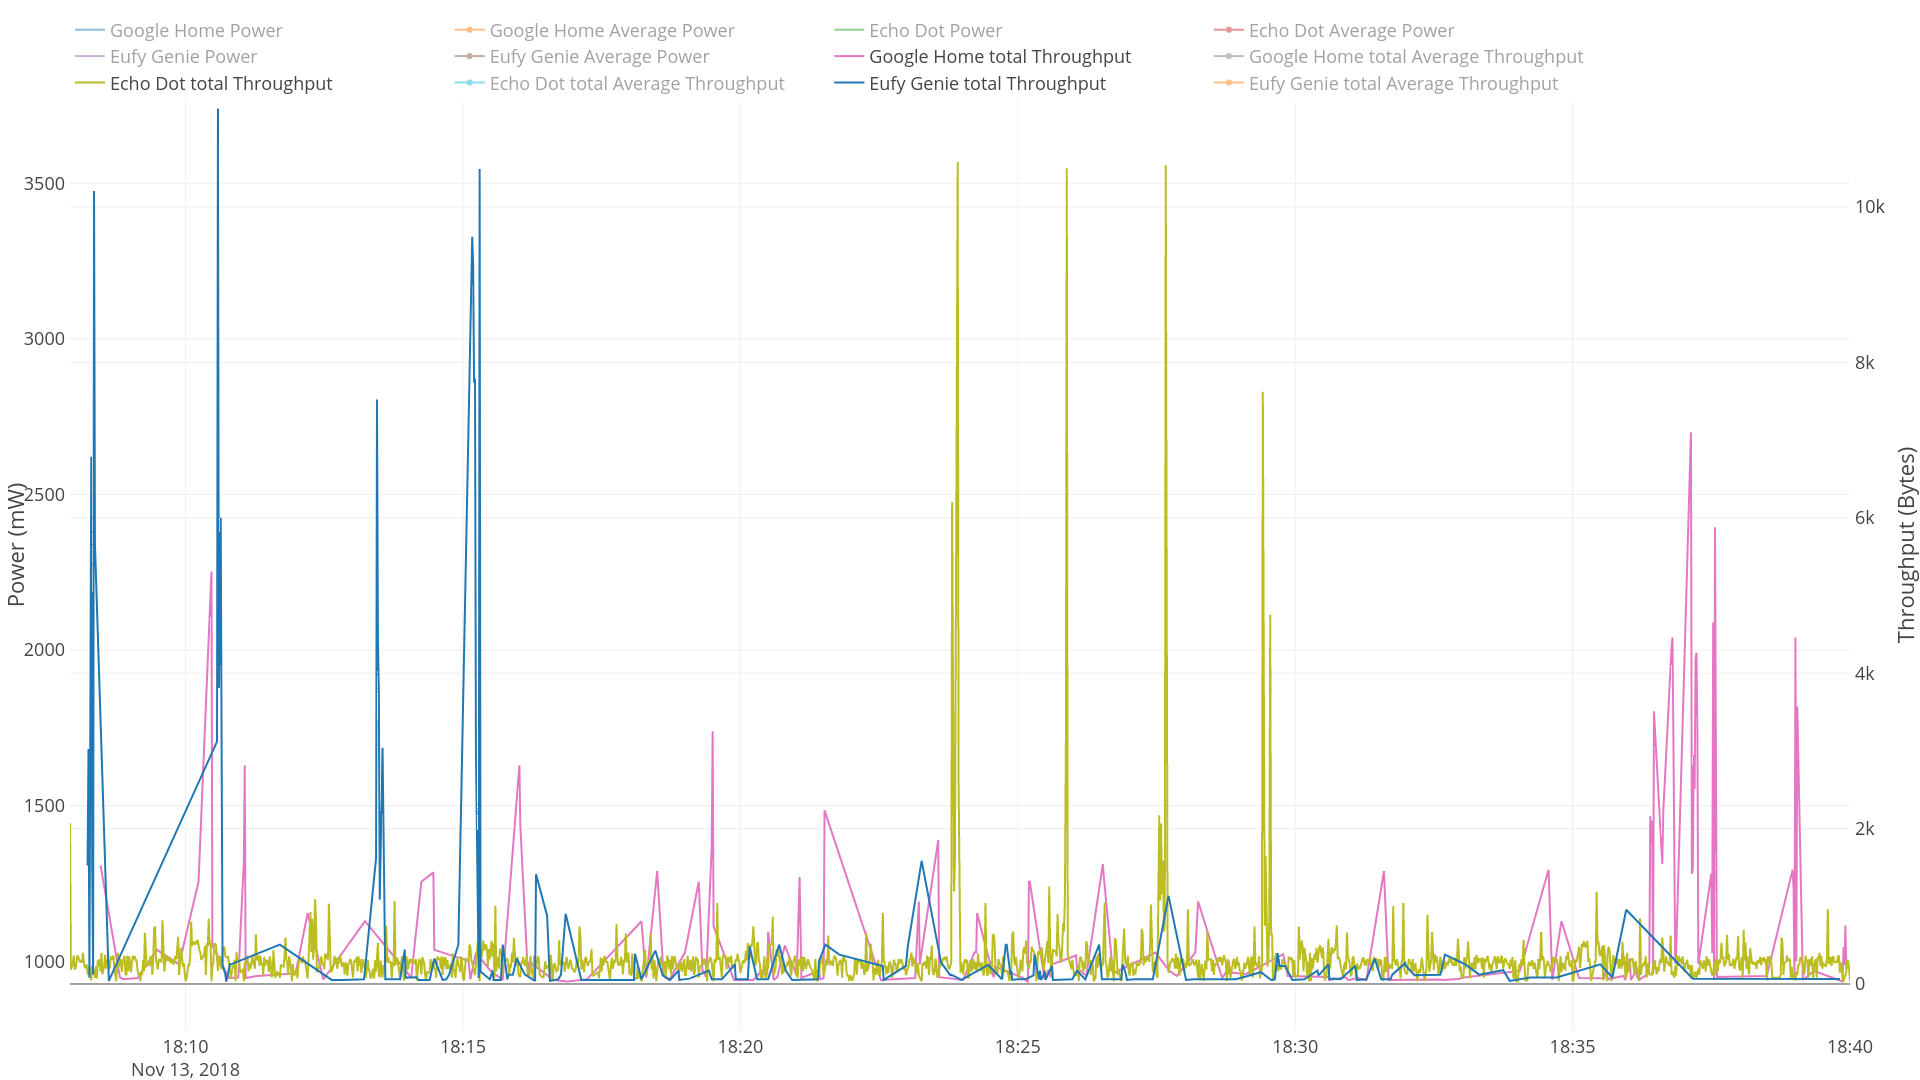
\includegraphics[width=1\textwidth]{figures/smartSpeakerNetworkSeperate.png}
  \caption{Power usage of Echo Dot 1, Eufy Genie 1, and Google Home over time when asked ``who is the best basketball player''. Same time frame as figure \ref{fig:smartSpeakerSeperate}}
  \label{fig:smartSpeakerNetworkSeperate}
\end{figure}

Finally, we noticed that the Echo Dot is characterized by a power spike that is a lot larger than the other smart speakers and wer interested to see what trade-offs these devices made.

From the results in section \ref{smartSpeakerComparisonSection}, we can see that the Echo uses the most power, then the Eufy, then the Google Home. However, the Eufy uses the most network throughput, then the Google Home, then the Echo Dot. We believe the Eufy is constantly communicating through the network so that it can cache results, minimizing onboard operations. The Echo Dot, on the other hand, uses the least network throughput and opts to do as much on board work as possible. The Google Home sits in the middle, querying the network, for more relevant things that it can cache for when the user asks the questions. It seems they pre-request results better. It is interesting that the Google Home still sits in the middle for network throughput when it is the only one that sends UPnP at such a high frequency. However, this is mostly speculation and would be interesting to see more research on this.

From the results in section \ref{smartSpeakerComparisonSection}, we can see that the Echo uses the most power, then the Eufy, then the Google Home. However, the Eufy uses the most network throughput, then the Google Home, then the Echo Dot. We believe the Eufy is constantly communicating through the network so that it can cache results, minimizing onboard operations. The Echo Dot, on the other hand, uses the least network throughput and opts to do as much on board work as possible. The Google Home sits in the middle, querying the network, for more relevant things that it can cache for when the user asks the questions. It seems they pre-request results better. It is interesting that the Google Home still sits in the middle for network throughput when it is the only one that sends UPnP at such a high frequency. However, this is mostly speculation and would be interesting to see more research on this.
\chapter{Conclusion}
\label{Conclusion}
To conclude, this paper documents the creation of a large database of IoT devices' network and power usage, introduces a graphing tool for this database and shows that it is possible to tell what smart speaker is in use based on just the initial spike made during a command.

After one year of logging common household IoT devices' network and power usage, our AWS database contains 172,445,929 entries that take up 184.94 GB of data. This database provides a large dataset for others to use without having to repeat the steps to form a testbed. This database was incredibly useful in Frawley and my work. Other students have already used it for their research projects.

To further streamline IoT research, a visualizer tool was created that graphs power and network usage for any device in the database, making visual analysis quick and easy. The visualizer provides many useful features that Frawley and I used for our research.

Some patterns can be difficult to make out with so much noise coming from within a house for power data. However, in some cases, it is still likely possible to determine what smart speaker is in use. With more research, it is likely that other private information can be inferred from the power line data as the research here has yet to leverage advanced statistical methods.

\section{Future Work}
With an ever-growing database, maintenance is necessary. We want to clean up the database by indexing all columns for quick lookup; as of now, only some columns are indexed. There are also some inconsistencies in the database because the IP addresses of the devices and WeMo names change over time. Unifying a device under one IP address and a WeMo under one name in the database are clear first steps.

The next plan is to improve the realtimeIoTgrapher and add features. The biggest interest is to add automatic annotations such as boxes denoting peak to peak spikes, or trend line plots. Plotly also has a feature to display the grapher on a public domain. Altering the grapher program to do so would also make this tool more easily accessible as compared to the locally hosted setup shown in this paper.

We also want to utilize both power and network data in tandem for analysis to see if even more information can be extracted.

With many botnet attacks in the recent past, we would like to hack into these devices with Mirai and analyze power usage and network throughput of these devices. This paper shows trends between power use, network traffic, and what an IoT device is doing. It is possible that power use and network traffic could correlate with Mirai's operations. Getting Mirai working in the restricted time turned out to be infeasible, but would be interesting to continue for future work.

Finally, applying advanced statistical methods to the power data would be interesting to pursue. We quickly tried machine learning with a feed-forward neural net with 0 percent accuracy and an LSTM and achieved 30 percent accuracy given five devices (slightly better than random). We had also planned to alter a human activity recognition machine learning (HAR) model to fit the database for classification of device model given power data over a set period. It is likely that machine learning can find patterns that visual examination could not.

Regardless, there are many opened opportunities for future work because of the database. There is already a student who is using the database for their research project. Researchers can quickly use the realtimeIoTGrapher to analyze the database or manually query data.

The world of IoT needs careful analysis and research for privacy and security. Hopefully, my contributions will help enable these studies.

\nocite{*}
\bibliography{bibliography}

% Indents Appendix in Table of Contents
\makeatletter
\addtocontents{toc}{\let\protect\l@chapter\protect\l@section}
\makeatother

% Hack to make Appendices to appear in Table of Contents
\addtocontents{toc}{%
   \noindent APPENDICES
}
\begin{appendices}
% \chapter{Source Code}
\label{source}
\lstinputlisting[language=Python]{appendices/sniff.py}

\end{appendices}

\end{document}
